% siminos/spatiotemp/chapter/blogSVW.tex
% $Author: predrag $ $Date: 2021-12-24 01:25:20 -0500 (Fri, 24 Dec 2021) $

% called by siminos/spatiotemp/blogCats.tex


\chapter{Sidney's blog}
\label{chap:blogSVW}

% Predrag                                       2020-12-27
%  moved GitHub cvitanov/reducesymm/kittens/sidney.tex to here
% Predrag                                       2020-08-18

\renewcommand{\Ssym}[1]{{\ensuremath{m_{#1}}}}    % Boris
\renewcommand{\Refl}{\ensuremath{{\sigma}}} % Dihedral wiki convention
\renewcommand{\shift}{\ensuremath{r}}
\renewcommand{\ssp}{\ensuremath{\phi}}             % lattice site field

	
{\large Sidney V.  Williams work blog}\\
swilliams425@gatech.edu\\
sidneywilliams1231@gmail.com\\
subversion siminos : swilliams425 \\ %spatioTemp \\
cell 208 310 3866

   % *********************************************************************
\hfill   {\color{red} The latest entry at the bottom for this blog}
\bigskip


\section{2020 blog}
\label{sect:sidney2020}

\bigskip

\begin{description}

\item[2020-05-20 Predrag] to Sidney:

You can write up your narrative in this file.
Can clip \& paste anything from above sections you
want to discuss, that saves you LaTeXing time.

\item[2021-09-09 Predrag]
The 3rd line of  \emph{siminos/spatiotemp/blogCats.tex}
says
\begin{verbatim}
% siminos/spatiotemp/inclOnlyCats.tex
% $Author: predrag $ $Date: 2021-12-18 15:14:03 -0500 (Sat, 18 Dec 2021) $

%%%%%%% Recompiling a smaller chunk %%%%%%%%%%%%%%%%%%%%%%%%%%
%%
%% Instead of recompiling the whole blogCats every time,
%% uncomment to compile only a chapter, or a subset of chapters
%%     (only one \includeonly{chapter/...} is allowed at a time)

% \includeonly{chapter/catMap}
% \includeonly{chapter/Henon}
% \includeonly{chapter/LC21}
% \includeonly{chapter/groups}
% \includeonly{chapter/catMapLatt}
% \includeonly{chapter/zeta2D}
% \includeonly{chapter/stability}
% \includeonly{chapter/action}
% \includeonly{chapter/chronotope}
% \includeonly{chapter/editing} % for CL18, GHJSC16 article comments
% \includeonly{chapter/symbolic}
% \includeonly{chapter/prime}
% \includeonly{chapter/appendStatM} % from ChaosBook: cat map chapter
% \includeonly{chapter/Ising}
% \includeonly{chapter/checkers}
% \includeonly{chapter/blogSVW}
% \includeonly{chapter/blogIA}
% \includeonly{chapter/blogXW}
% \includeonly{chapter/blogHL}
% \includeonly{chapter/reportRJ}
% \includeonly{chapter/reportAKS}
% \includeonly{chapter/blogRJ}
% \includeonly{chapter/blogAKS}
% \includeonly{chapter/dailyCats}
% \includeonly{chapter/powwows}

% \includeonly{chapter/catMap,chapter/catMapLatt}
% \includeonly{chapter/catMap,chapter/catMapLatt,chapter/dailyCats}
% \includeonly{chapter/catMap,chapter/blogHL}
% \includeonly{chapter/catMap,chapter/Henon,chapter/blogSVW,chapter/blogHL,chapter/powwows}
% \includeonly{chapter/catMap,chapter/Henon,chapter/LC21,chapter/groups,%
%              chapter/action,chapter/blogSVW,chapter/blogHL}
% \includeonly{chapter/catMap,chapter/prime,chapter/blogHL}
% \includeonly{chapter/catMap,chapter/blogHL,chapter/dailyCats}
% \includeonly{chapter/catMap,chapter/catMapLatt,chapter/blogHL}
% \includeonly{chapter/catMap,chapter/blogHL,chapter/Ising}
% \includeonly{chapter/catMap,chapter/groups,chapter/editing,chapter/blogHL}
% \includeonly{chapter/catMap,chapter/Henon,chapter/groups}
% \includeonly{chapter/catMap,chapter/blogSVW,chapter/blogHL,chapter/powwows}
% \includeonly{chapter/catMap,chapter/catMapLatt,chapter/Henon,%
%               chapter/stability,chapter/action,chapter/blogSVW,%
%               chapter/blogHL,chapter/powwows}
% \includeonly{chapter/catMap,chapter/catMapLatt,chapter/stability,
%              chapter/chronotope,chapter/action,
%              chapter/prime,chapter/Ising,chapter/blogHL,chapter/dailyCats}
% \includeonly{chapter/catMapLatt,chapter/Ising,chapter/dailyCats}
% \includeonly{chapter/catMapLatt,chapter/groups,chapter/blogHL}
% \includeonly{chapter/catMapLatt,chapter/Ising}
% \includeonly{chapter/catMapLatt,chapter/chronotope,chapter/Ising}
% \includeonly{chapter/catMapLatt,chapter/blogHL}
% \includeonly{chapter/catMapLatt,chapter/stability}
% \includeonly{chapter/catMapLatt,chapter/stability,chapter/action,chapter/Ising,chapter/blogHL}
% \includeonly{chapter/LC21,chapter/groups}
% \includeonly{chapter/LC21,chapter/groups,chapter/blogHL}
% \includeonly{chapter/Henon,chapter/LC21,chapter/groups,chapter/blogSVW,chapter/blogHL}
% \includeonly{chapter/stability,chapter/action}
% \includeonly{chapter/chronotope,chapter/dailyCats}
% \includeonly{chapter/blogHL,chapter/dailyCats}
% \includeonly{chapter/blogHL,chapter/dailyCats,chapter/powwows}
% \includeonly{chapter/symbolic,chapter/blogHL}
% \includeonly{chapter/Henon,chapter/blogSVW}
% \includeonly{chapter/Henon,chapter/blogSVW,chapter/blogHL}
% \includeonly{chapter/Henon,chapter/LC21,chapter/groups,chapter/catMapLatt,chapter/blogSVW,chapter/blogHL} %,chapter/powwows}
  %process only the files you are editing
\end{verbatim}
you uncomment a single line in that file to "process  only the files you
are editing".
% Don't comment out files called further down by the
% masterfile \emph{blogCats.tex}, that can get confusing for other people.

\item[2021-07-04 Predrag to Sidney]
Pro tip: compile \emph{blogCats.tex} often, as you write, and fix errors as
you write. I had to go all they way back to May to find one of your
unbalanced ``$\{$'' and make the entire blog compile without errors...

\item[2020-08-22 Predrag]
First task:

Start reading kittens/CL18.tex\rf{CL18} sect.~%{s:Bernoulli}~
{\em Bernoulli map}.
Everything up to CL18 sect.~{s:1D1dLatt}
{\em Temporal Bernoulli}
you know from the ChaosBook course.

New stuff starts here. See how much you understand. Write your
study notes up here, ask questions - this is your personal blog.

You refer to an equation like this: CL18 eq.~{tempBern};

to figure like
this: CL18 figure~{fig:BernCyc2Jacob};

to table like this:
\reftab{tab:LxTs=5/2};

to a reference like this: Gutkin and Osipov\rf{GutOsi15} (\emph{GutOsi15}
refers to an article listed in \emph{../bibtex/siminos.bib}).

and to external link like this:
``For great wallpapers, see overheads in
\HREF{http://www-personal.umich.edu/~engelmm/lectures/ShortCourseSymmetry.html}
{Engel's} course\rf{Engel11}.''

\item[2020-08-22 Predrag] An example of referring to the main text:
Why do you write \emph{\jacobianOrb}
CL18 eq.~{jacobianOrb} as a partial derivative, when you already
know $\jMorb$, see CL18 eq.~{tempFixPoint}?

\item[2020-08-24 Sidney]~
Started reading from the beginning as that only adds an additional 4 pages, and it would be beneficial to review.

\vspace{3mm}

General Notes:
Showing what modern chaos calculations look like.
The \catlatt\ is the arbitrary dimension generalization of the 1-D Bernoulli map.

(mod 1) subtracts the integer part of $s\field_t$, this keeps $\field_{t+1}$
within the unit interval (group theoretic analogue?). Also partitions
the state-space into $s$ sub-intervals.

\item[2020-08-24 Predrag]
The group theory here compatifies translations on the (infinite) line
$\field\in(-\infty,\infty)$ to translations on the (compact) circle
$\field\in[0,2\pi)$.

\item[2020-08-24 Sidney]~
Reminder to self: review the symbolic dynamics, and binary operations from
chapter 14 of Chaosbook The unit interval is partitioned into $s^n$
subintervals, each with one unstable period-n point, except the rightmost
fixed point is the same as the fixed point at the origin. So there are
$s^n-1$ total period-n periodic points. $\shift$ in \refeq{tempBern} is a
cyclic permutation that translates forward in time the {\lattstate} by one
site. Inverse $\shift$ because the second term is always one step behind the
first term and an inverse $\shift$ moves the state back one.
\vspace{3mm}

Questions
1. I've pretty much never done modular arithmetic before, I understand CL18 eq.~{BerStretch} in the idea that the circle map wraps in on itself and contributes the value of its slope after one go around, but I am unsure on how to use the modular arithmetic to do that, should I look into that?

\item[2020-08-24 Predrag]
As I do not know what ``modular arithmetic'' is, don't worry about :)

\item[2020-08-25 Sidney]~
General Notes

CL18 eq.~{pathBern} appears to be a vector of a periodic (or relative
periodic orbit) through the Bernoulli map. Review Multishooting. Total
number of of periodic points of period n is $N_n=s^n-1$ but it also
equals the magnitude of the determinant of the {\jacobianOrb}.
(got to page 7)

\vspace{3mm}

\begin{itemize}
  \item[Q1]
Is CL18 eq.~{tempBernFix} the evolution function $f^t(y)$ that was
referenced throughout ChaosBook?
  \item[Q2]
What exactly is meant by a ``lattice"?
\end{itemize}

\item[2020-08-24 Predrag].

\begin{itemize}
  \item[A1]
The whole point of the paper us that ChaosBook is obsolete - in the new
formulation, there is no `time' evolution, no time trajectory $f^t(y)$,
there are only sets of fields the live on lattice points that satisfy
recurrence relations. CL18 eq.~{tempBernFix} is \emph{\jacobianOrb}, the
stability of a {\lattstate}, to be related to stability forward in time
in CL18 sect.~{s:Hill}. This is a revolution: there is no more time, there
is only spacetime.
  \item[A2]
Temporal lattice $\integers$ is defined in CL18 eq.~{pathBern}. Spacetime
integer lattice $\integers^2$, (or more generally $\integers^d$) in
CL18 eq.~{KanekoCML}, CL18 eq.~{CatMap2d}.
When you get to it, a 2\dmn\ \emph{Bravais lattice} $\Lambda$ is defined
in CL18 eq.~{2DBravaisLattice}.

If this is unclear, read up on integer lattices, give your own precise definition.
\end{itemize}

\item[2020-08-26 Sidney]~
Point Lattice (integer lattice is a special case of point
lattice) notes from
\HREF{https://mathworld.wolfram.com/PointLattice.html}{Wolfram}: "A point
lattice is a regularly spaced array of points." The integer lattice is
where all of these points are integers. I will look at the Barvinok
lecture tomorrow, I have to finish moving to a different house today.
(Stayed on page 7)

\begin{itemize}
	\item[Q3]
Please correct me if I am wrong, but a lattice seems to be a collection
of points where are all regularly spaced, so does "regularly" mean that
it is controlled by a deterministic law? If this is the case, the
$\ssp_n$ states in a periodic orbit can be grouped as a lattice and
ordered by location along the periodic orbit, then the associated
"winding" number $\Ssym{\zeit}$ can be grouped in its own lattice, which in this
case is an integer lattice. What is the "regular" spacing for the winding
numbers? Have missed the point?
\end{itemize}

\begin{itemize}
  \item[A3]
Wolfram is right. When you have a discrete time map, time takes integer
values $\zeit=\cdots,-1,0,1,2,\cdots$. That is called 1\dmn\ integer lattice
$\integers$. Once you are in $d=2$ or higher, the name makes sense, as
you can visualize $\integers^2$ as a `lattice'. It is regular, because all spacings
between neighboring points are 1. There is nothing `deterministic' about
this, it just says that time takes its values on integers, rather than on a continuum.

There is only one lattice, but on each lattice site there is a
real-valued field $\ssp_\zeit$ and the integer valued `source' \Ssym{\zeit}.
\end{itemize}

\item[2020-08-27 Sidney]~
Thank you for A1, that makes complete sense now. Calculated the {\jacobianOrb}
using equation CL18 eq.~{tempBernFix}, matched with the paper, yay.
{\JacobianOrb} maps the basis vectors of the unit hyper-cube into a
{\fundPip} basis vectors, each of which is given by a
column in the {\jacobianOrb}. $|\Det(s/\shift|=s^n$ because $\shift$ and
its inverse are both unitary matrices, and if you multiply every row of
an $[n\times{n}]$ matrix, the determinant is multiplied by the constant
raised to the power n. Periodicity $\shift^n=1$ accounts for
$\overline{0}$ and $\overline{s-1}$ fixed points being a single periodic
point. (got to page 9)

\begin{itemize}
	\item[Q4]
I was trying to calculate the {\jacobianOrb} using the $\shift$ matrix, but the delta function equation CL18 eq.~{hopMatrix} for $\shift$ doesn't seem to work for the Bernoulli map, I know that $\shift_{2,1}=1$ and $\shift_{1,2}=1$ which works with the delta function definition. However, $\shift_{2,1}=\delta_{3,1}$ from CL18 eq.~{hopMatrix}, which should equal zero. Other than just the idea of being cyclic, I don't know why it yields one instead of zero, what am I missing?
  \item[A4]
Work it out $\shift$ matrices for $n=1,2,3,\cdots$. It will start making sense.
	\item[Q5]
So, does ``{\lattstate}" mean the set of all points (field of all points?) which running through the Bernoulli map requires the specific winding number at that lattice site?
  \item[A5]
Interesting, grad students too seem to confuse coordinates (for example,
$(x,\zeit)=(3.74,-0.02)$ in continuum, $(n,\zeit)=(7,-6)$ on a discrtized space)
and the
fields $\ssp(n,\zeit)$. Physical ``state'' refers to value of field $\ssp$
over every $(n,\zeit)$ - is the grass high or low? rather than the coordinates
of spacetime.

How would you state this precisely if you were trying to explain this
paper to another student?
\end{itemize}

\item[2020-08-30 Sidney]~~
\begin{itemize}
  \item[A5.1]
Sidney: ``
$\Xx_\Mm$ is the set of all values the field $\ssp_z$ takes over
the set of coordinates $\Mm$.
% Please let me know if I have missed something here.
''
  \item[A5.2]
Predrag: Please reread 2nd paragraph of CL18 sect.~{s:1D1dLatt} and explain what
is wrong with your answer A5.1
\end{itemize}

\vspace{3mm}

Notes: For an period-$\cl{}$ {\lattstate} $\Xx_\Mm$ the Jacobian
matrix is now a function of a [d x d] matrix J, so the formula for the
number of periodic points of period n (number of {\lattstate}s of period
n) is now $|\det(1-J_M)|$ where $J_M=\prod^n_{t=1}J_t$ where $J_t$ is the
one-step Jacobian matrix which is assumed to vary in time.

\begin{itemize}
	\item[Note to self:]
look back over the topological zeta function, specifically try to
understand derivation of:
\[
\frac{1}{\zeta_{top}(z)}=\exp\left(-\sum^{\infty}_{n=1}\frac{z^n}{n}N_n\right)
\]
(got to CL18 page~{s:bernODE})
	\item[Predrag:]
\toChaosBook{section.18.4} {(click here)}
	\item[Q6]
Is ``there are ${s}$ fundamental {\lattstate}s, and every other {\lattstate}
is built from their concatenations and repeats"
is simply a restatement of the fact that the Bernoulli map is a full shift?
	\item[A6]
For Bernoulli, yes. But search for word `fundamental' in
\toChaosBook{chapter.18}
{{\em Counting}}. For example, `We refer to the set of all
non-self-intersecting loops $\{ t_{p_1}, t_{p_2}, \cdots t_{p_f} \}$ as
the {\em fundamental cycles}'. Write up here a more nuanced statement of
`fundamental' cycles might be (I do not have firm grip on this either...).
	\item[Q7]
Is CL18 eq.~{bernN\_n-s=2} a result of expanding in a Taylor the result
of the derivative (and product of $1/\zeta_{top}$ and $z$)? Because the
topological zeta function of the Bernoulli map is a closed form function,
not an infinite sum.
\end{itemize}

\item[2020-08-31 Sidney]~
Via a finite difference method, CL18 eq.~{1stepDiffEq} can be viewed as a
first order ODE dynamical system. Back-substituted with \refeq{tempBern}
to show that with $\Delta t=1$ the velocity field does satisfy the diffeq
\refeq{exam:1stepVecEq}.
The Bernoulli system can be recast into a discretized ODE whose global
linear stability is described by the {\jacobianOrb}.
(Stayed on CL18 page~{s:bernODE}))

\item[2020-09-01 Sidney]~
Started reading CL18 sect.~{s:kickRot}~{\em A kicked rotor}.

\refeq{PerViv2.1b}
and \refeq{PerViv2.1a} describe the motion of a rotor being subjected to
periodic momentum pulses. The mod is present for the q equation to make
sure that the angle varies from $0$ to $2\pi$. As in the Bernoulli map case,
here
mod is also added to the momentum equation to keep it bounded to a unit
square. Cat maps with the stretching parameter ${s}$ are the same up to a
similarity transformation. An automorphism is an isomorphism of a system
of objects onto itself. An isomorphism is a map that preserves sets and
relations among elements.

\begin{itemize}
	\item[Q8]
Do the kicked rotor equations with Hooke's law force, and bounded momentum (mod 1 added to CL18 eq.~{PerViv2.1a}) only take the form of CL18 eq.~{catMap} if K is an integer?
	\item[A8]
The text states: ``The
$(\mbox{mod}\;1)$ added to CL18 eq.~{PerViv2.1a} makes the map a
discontinuous `sawtooth,' unless $K$ is an integer.'' How would you make that clearer?
	\item[Q9]
How does CL18 eq.~{catMap} have a state space which is a 2-torus? I am having a hard time visualizing how this came about.
	\item[A9]
Do you understand how  $(\mbox{mod}\;1)$ operation turns unbounded stretch
CL18 eq.~{BerStretch} into a circle map CL18 eq.~{n-tuplingMap}? Circle map is
1-torus. If both
\(
(\coord_{\zeit},p_{\zeit}) \in  (0,1]\times(0,1]
\)
are wrapped into unit circles, the phase space $(\coord_{\zeit},p_{\zeit})$
is not an infinite 2\dmn\ plane, but a compact, doubly periodic unit square with
opposite edges glued together, \ie, 2-torus.
\end{itemize}

%	\item[2020-09-02 Predrag]
%Your every commit's description is ``Update sidney.tex'',
%while my commits describe the edits. ``Update sidney.tex'' is not
%informative, especially later, if you try to find a particular commit...

\item[2020-09-03 Sidney]~
I was typing my description into "summary" textbox above the commit to
master button. Obviously I was incorrect, I'll try to type in the
"description" for this commit.

\item[2020-09-02 Predrag]
``Tripping Through Fields'' showed up :)

\item[2020-09-03 Sidney]~~
\begin{itemize}
	\item[A5.3] Sidney:
I'm not actually quite sure what's wrong with my given definition. From
your answer A5 it seems that \Mm\ is a set of
coordinates (the location of the blade of grass) and $\Xx_\Mm$ is
the value at that coordinate (the height of the grass at that point).
Perhaps I forgot that these {\lattstate}s are for periodic orbits, so I
forgot the second coordinate (period of length n).
	\item[A5.4] Predrag: %2020-09-03
The textbook inhomogeneous \emph{Helmoltz equation} is an elliptical
equation of form
\beq
   (\Box+k^2)\,\ssp(z)= -\m(z)\,,\qquad z\in \reals^d
\,,
\label{CatMapContinuesPC}
\eeq
where the \emph{field} $\ssp(z)$ is a $C^2$ functions of
\emph{coordinates} $z$, and $\m(z)$ are \emph{sources}. For example,
charge density is a \emph{source} of electrostatic \emph{field}.

Suppose you are so poor, your computer lacks infinite memory, you only
have miserly only 10\,Tb, so you cannot store the infinitely many values
that \emph{coordinates} $z\in \reals^d$ take. So what do you do?

Perhaps a peak at ChaosBook
\toChaosBook{section.X.1} {~A24.1
Lattice derivatives} can serve as an inspiration. And once you have done
what a person must do, your Helmoltz equation (hopefully) has the form of
CL18 eq.~{OneCat}.
What is a \emph{field}, a \emph{source}, a \emph{coordinate} then?
\end{itemize}


\item[2020-09-03 Sidney]~~
\begin{itemize}
	\item[A8.1]
The sawtooth statement made sense, what made it unclear for me was the second sentence which started with "in this case" it was (again for me, I might not have been paying enough attention) ambiguous, I didn't know if it was talking about the integer case or the sawtooth case.  	
	\item[A8.2] Predrag: thanks, I rephrased that sentence.
	\item[A9.1]
I understand, your explanation makes sense, thank you :).
\end{itemize}

\vspace{3mm}

Notes: The discrete time Hamiltonian system induces forward in time evolution
on the 2-torus phase space. The {\jacobianOrb} can take many different forms
depending on the map. Despite this the {\HillDet} can still count the
number of {\lattstate}s.
(got to page CL18 page~{s:tempCatCountTEMP})

\item[2020-09-05 Sidney]~~
\begin{itemize}
	\item[A5.5]
If I was so unlucky to only have 10Tb of memory, I would take a finite
interval of points z that I was interested in, and discretize them
(evenly, or unevenly) and then evaluate the field (that was probably the
wrong wording) at a finite set of points, either of particular interest
within the interval, or closely spaced enough so that the values were
representative of the values the field took over a continuum. I think
that a coordinate is a point in state space specified by specific values
of state variables (position, time, momentum etc.). To try to answer
source, and field, I'll be thinking of an electric charge, a source is
what generates the medium by which other sources are effected, and the
field is the medium which acts upon other sources.

	\item[A5.6]
I did look at
\toChaosBook{section.X.1}
{A24.1 Lattice derivatives}, but it didn't seem to address quite the
fundamental confusion I seem to be facing. I'm relatively confident in my
coordinate definition, but not at all in my source, and field definition.
\end{itemize}

\item[2020-09-05 Predrag].
\begin{itemize}
	\item[A5.7]
Expression ` state space' $\pS$ refers to `states': cats, dancers,
\ie, `fields' \Xx\ and their
names \Mm. `Coordinates' refer to markings on the floor that they stand on.

Does reading CL18 sect.~{s:lattState}~{\em {\Lattstate}s} now helps in
distinguish a skater from the skating ring's ice? I rewrote it for your
pleasure :)
	\item[A5.7]
Re. the fundamental confusion of reading
\toChaosBook{section.X.1} {A24.1
Lattice derivatives}: If you mark every inch on the floor, this is
`discretization'. But the floor is still a floor, no?
\end{itemize}

%\item[2020-09-05 Predrag] It looks like you do not use `diff' to find out
%what has been edited. Also, GitHub Desktop shows the edited text by coloring
%it. I keep edition your text to help you learn the macros used in writing
%the article.
%
%\item[2020-09-05 Sidney]~
%I see why you do the editing, I'll try to incorporate the fancier
%\LaTeX{} footwork into my blog.

\item[2020-09-05 Sidney]~~
\begin{itemize}
	\item[A5.8]
I read the pink bits of CL18 sect.~{s:lattState}~{\em {\Lattstate}s} (as I
assume that was the parts that you rewrote specially). From it I (think)
I understand. We're looking at two coordinates for most of the Bernoulli
and cat map stuff: a spatial one, and a temporal one, the maps only
effect the temporal placement, but effect it differently depending on
where the point was in space when the map acted on it, because the field
takes a different value at every point in space (and time). So the
coordinates are the field point placement in time and space. The field is
the value that is assigned to every lattice point. \Mm\ keeps getting
referred to as an alphabet, so that makes me think that it is similar
(perhaps the multidimensional generalization) to the ``alphabet" which was
used to partition state space in the 1D maps of Chaosbook, such as 0 for
the left half of the interval and 1 for the right, and then further
partitioning the more the map is applied. Is that close at least?
\end{itemize}

\item[2020-09-05 Predrag].
\begin{itemize}
	\item[A5.9]
Getting hotter. Look at CL18 eq.~{circ-m} and CL18 eq.~{catMapNewt};
$\ssp_{\zeit}$ and $\Ssym{\zeit}$ are the same kind of a beast,
$\Ssym{\zeit}$ is just the integer part of the ``stretched'' field in
CL18 eq.~{BerStretch}. In this particular, linear map setting, this integer
does double duty, as a letter of an ``alphabet''. It cannot possibly be a
``coordinate'', it like saying that a dancer's head is ``floor.''
	\item[A5.10]
In temporal lattice formulation no ``map is applied.'' That is the
brilliance of the global \spt\ reformulation: there is no stepping
forward in time, so there is no map - the only thing that exists is the
global fixed point condition that has to be satisfied by field values
everywhere on the lattice, simultaneously.

Time is dead.
\end{itemize}

\item[2020-09-08 Sidney]~~
\begin{itemize}
	\item[Q11]
So the \templatt\ / \catlatt\ equations are moving around points in the lattice instead of
through time?
	\item[Q12]
Is something of the form of CL18 eq.~{tempFixPoint} an example
of the ``global fixed point condition"?
\end{itemize}

\item[2020-09-14 Predrag].
\begin{itemize}
	\item[A11]
An equation does not have to be ``moving around'' anything: think of a
quadratic equation $x^2+bx+c=0$. Does it ``move'' anything? No. It's a condition
that a single ``field'' $x$ has to satisfy, and the solution is a root of that
equation.
The \templatt\ / \catlatt\ equations are ``equations'' in the same sense,
[bunch of terms involving $\ssp_z$ ]=0.
	\item[A12]
Yes.
\end{itemize}

\item[2020-09-09 Sidney]~
Notes: Equations such as CL18 eq.~{catMapNewt} can be solved using similar methods to linear odes: guessing a solution of the form $\Lambda^t$ and finding the characteristic equation. Then assuming all terms are site independent because the difference of any two solutions of CL18 eq.~{catMapNewt} solve its homogeneous counterpart CL18 eq.~{diffEqs:CatCharEq}. Got to CL18 page~{s:tempCatZeta}.

Notes: Topological zeta functions count {\orbit}s, i.e. time invariant sets of equivalent {\lattstate}s related by cyclic permutations. The "search for zeros" CL18 eq.~{tempCatFixPoint} is the "fixed point condition." Which is a global statement which enforces CL18 eq.~{catMapNewt} at every point in the lattice. Got to CL18 page~{s:catlatt}

\item[2020-09-13 Sidney]~
The \templatt\ is a special case of the \catlatt, defined on a one\dmn\
lattice $\integers^1$. In this case the associated topological zeta
function is known in a closed, analytic form.

\emph{Coupled map lattices}: Starts with a review of finite difference
methods for PDEs. The d dimensions in the lattice are d-1 spatial lattice
points and 1 temporal one. The PDE is reduced to dynamics of a coupled
map lattice, with a set of continuous fields on each site.

\begin{itemize}
	\item[A5.11]
I have experience with finite difference methods for solving a
discretized form of a PDE, but I'm having a hard time visualizing the
idea of having a discrete coordinate system in d different directions,
but with a continuous field on each site. This  may be valuable as it is
a specific statement of where I'm getting stuck.
	\item[Q13]
My current understanding is
that at each point in the d-dimensional integer lattice ("point" as in a
lattice node with d specified coordinates), but at each point (site)
there is a continuous field. What is this field continuous over? It's at
one point in a discrete coordinate system. And why is there a continuum
at each point? And finally, I assume that these continuous fields are the
values of the function being solved for at that point, however, shouldn't
that just be a single value? Not a field? I'm sorry if this is a rather
silly question, but I'll keep thinking about it and I'll make a note if
my understanding (or lack thereof) changes.
	\item[A13]
Predrag: In CL18 \reffig{fig:BernPart} field $x_\zeit$ or $\ssp_\zeit$ and
$f(\ssp_\zeit)$  on the discrete site $\zeit$ run over continuous values.
For example, at temporal lattice site $\zeit=7$ the field value is
$\ssp_7=0.374569263952942\cdots$. OK now?
	\item[Q13.1]
Slight update, it seems that the field is the state of the system and at each discretized point there is a map acting on the state, although that conflicts with the notion that time is dead, so I'm probably still misunderstanding.
	\item[A13.1]
Predrag: Yes.
\end{itemize}
Thinking of this as a spring mattress. Often starts out with chaotic on-site dynamics weakly coupled to neighboring sites.
In this paper one sets the lattice spacing constant equal to one. Diffusive coupled map lattices introduced by Kaneko:
\[
\ssp_{n,t+1}=
g(\ssp_{n,t})+\epsilon\left[g(\ssp_{n-1,t})-2g(\ssp_{n,t})+g(\ssp_{n+1,t})\right]
\,,
\]
where each individual spatial site's dynamical system $g(x)$ is a 1D map, coupled to the nearest neighbors by the discretized second order \emph{spatial} derivative. The form of time-step map $g(\ssp_{n,t})$ is the same for all time i.e. invariant under the group of discrete time translations. Spatial stability analysis can be combined with temporal stability analysis, with orbit weights depending exponentially both on the space and the time variables: $t_p\propto e^{-L\period{}\lambda_p}$. $\shift_i$ translates the field by one lattice spacing in the $i^{th}$ direction.
\begin{itemize}
	\item[Q14]
What is a lattice period?
	\item[A14]
Predrag: Does the paragraph above CL18 eq.~{catlattFix} answer you question?
I would like to refer to the \emph{set} of numbers
$\{\ell_1,\ell_2,\cdots,\ell_d\}$ as the \emph{period} of lattice
$\Lambda$. Would that be confusing?
	\item[Q15]
Is $z$ in the definition of a {\lattstate} both a temporal and a spatial index? So equivalent to both n and t?
	\item[A15]
Predrag: after CL18 eq.~{CatMap2d} I write ``a 1\dmn\ spatial
lattice, with field $\ssp_{n\zeit}$ (the angle of a kicked rotor
\refeq{PerViv2.1b} at instant $\zeit$) at \spt\ site
$z=(n,\zeit)\in\integers^2$.'' Should this
``$z=(n,\zeit)\in\integers^2$'' be repeated elsewhere. If so, where?
	\item[Q16]
Often a member of the alphabet can be a negative number, which I assume
means that the state is taken out of unity in the negative direction.
	\item[A16]
Do you understand CL18 figure~{fig:BernCyc2Jacob} and CL18 figure~{fig:catCycJacob}?
\end{itemize}

The
\catlatt\ has the point-group symmetries of the square lattice.
A {\lattstate} is a set of all field values $\Xx=\{\ssp_z\}$ over the
d-dimensional lattice that satisfies the \catlatt\ equation,
with all field values constrained between zero and one. A {\lattstate}
$\Xx_{\Lambda}$ is a \emph{\twot} if it satisfies
$\Xx_{\Lambda}(z+R)=\Xx_{\Lambda}(z)$ for any
discrete translation $R=n_1\mathbf{a}_1+n_2\mathbf{a}_2 \in \Lambda$. Got
to CL18 page~{s:catLatt1x1}.

\item[2020-09-14 Sidney]~~
\begin{itemize}
	\item[A13.1]
I think I'm OK now. I think what I was trying to visualize was a stack of an infinite number of values at each lattice point, which was confusing, but this makes sense.
	\item[A14.1]
Unfortunately I don't think I quite understand. I understand the idea of the different directions, I understand treating
$\Xx_\Mm(\ssp_z)$ as a singular fixed point, but I do not understand $\ell_i$.
	\item[A15.1]
I think that I lost that definition of $\textit{z}$ around CL18 eq.~{dDCatsT}, but I think that may have been a factor of how long it takes me personally to digest this material.
	\item[A16.1]
After reading the descriptions and staring at it for awhile, I think that I do.
	\item[Q17]
I tried a couple days back (Thursday or Friday I think, they all blend together) to log in to your bluejeans office. But it must have been one of the times that it had logged you off due to inactivity. There was also another person their I didn't recognize, and I didn't want to step on their toes if they were waiting for you to get back, so I logged off. So, when in general would good times to try hopping into your office?
\end{itemize}

\item[2020-09-16 Sidney]~
A Bravais lattice can be denoted $\Lambda=\left[L\times\period{}\right]_S$ where $L$
is the spatial lattice period,  $\period{}$ is the temporal lattice period, $S$
imposes the tilt to the cell. Basis vectors for the Bravais cell can be
written as:
\[
\mathbf{a}_1=\left(\begin{array}{c}
  \speriod{}\\
  0{}
  \end{array}\right)
  \,,\qquad
\mathbf{a}_2=\left(\begin{array}{c}
  \tilt{}\\
  \period{}
  \end{array}\right)
  \,
\]

\begin{itemize}
	\item[Q18]
If something is written as $850[3\times2]_0$ what is the numerical value?
More importantly, how is it found? I know it has to do with the cyclic
permutations of the prime blocks, but I'm not sure how to get a numerical
value.
\end{itemize}
Got to page CL18 page~{s:catLattCount}

\item[2020-09-17 Sidney]~
For the Bernoulli map its stretching uniformity allows the use of
combinatorial methods for lattice points. For temporal (not spatiotemporal)
the number of {\lattstate}s is the same as the volume of the
{\fundPip}, so the magnitude of the determinant of the {\jacobianOrb}. The
block $\Mm$ can be used as a 2D symbolic representation of the lattice system
state. For a given admissible source block $\Mm$, the periodic field can be
computed by:
\[
\ssp_{i_1j_1}=\sum_{i_2=0}^2\sum_{j_2=0}^1\mathbf{g}_{i_1j_1,i_2j_2}\Mm_{i_2j_2}
\]


\item[2020-09-19 Predrag]
Sorry, I've been a bit overwhelmed with lecture preparations, so
I will not answer any of the questions quite yet. But I have rewritten the
abstract, and the introduction to the paper, up to
the start of CL18 sect.~{s:Bernoulli}~{\em Bernoulli map}.
Can you have a critical look at the new text, report here if
something does not make sense to you?

\item[2020-09-19 Sidney]~~
%Sure, I'll add to this blog post if anything throws me. Don't worry about being busy, I understand.
\begin{itemize}
	\item[Update]
I read through, and aside from some very minor grammar issues (forgetting
a ``have" after ``we")
% and forgetting a closed parentheses etc. PC fixed that one
it all makes sense.
\end{itemize}

\item[2020-09-20 Predrag].
\begin{itemize}
	\item[A15.2]
I now added the $z$ definition to CL18 eq.~{dDCatsT},
is that clearer?
\end{itemize}

\item[2020-09-20 Sidney]~~
\begin{itemize}
	\item[A15.3]
Yes, that makes it clearer.
\end{itemize}
$$-\sum^{\infty}_{r=1}\frac{1}{r}\tr\hat{\mathbf{J}}_p^r
=\tr\left(-\sum^{\infty}_{r=1}\frac{1}{r}\hat{\mathbf{J}}_p^r\right)
= \tr\hspace{2mm}\ln\left(\hat{1}_1-\hat{\mathbf{J}}_p^r\right)
= \ln\hspace{2mm}\det\left(\hat{1}_1-\hat{\mathbf{J}}_p^r\right)$$
I liked the text cut from the introduction on page 44, it made the idea of time's death more easily digestible. Finished main paper, will look at the appendices for math.

\item[2020-09-22 Sidney]~~
\begin{description}
\item[Math Review Part 1]
\item[Updated 9/29/20]
\item[Bravais Lattice]

From \HREF{https://en.wikipedia.org/wiki/Bravais_lattice}{Wikipedia}:
A Bravais lattice is an infinite array of discrete points generated by a
set of discrete translation operations described in two dimensional space
by:
$$\mathbf{R}=n_1\mathbf{a}_1+n_2\mathbf{a}_2$$
where $n_i$ is any integer and $\mathbf{a}_i$ is a primitive vector, each
$\mathbf{a}_i$ lie in different directions, but are not necessarily
mutually perpendicular, but they do span the lattice. A fundamental
aspect of a Bravais Lattice is that no matter the direction of the
primitive vectors, the lattice will look exactly the same from each of
the discrete lattice points when looking in that direction. A Lattice is
is a periodic array of points where each point is indistinguishable from
any other point and has identical surroundings. A unit cell expands the
idea of the infinite array of discrete points to include the space
inbetween the points, if we are looking at a physical system this
includes the atoms in this space. There are two main types of unit cells:
primitive unit cells and non-primitive unit cells. A unit cell is the
smallest group of atoms of a substance that has the overall symmetry of a
crystal of that substance, and from which the entire lattice can be built
up by the repetition in three dimensions. A primitive cell must contain
only one lattice point, generally, lattice points that are shared by $n$
cells are counted as $\frac{1}{n}$ of the lattice points contained in
each of those cells. So traditional primitive cells only contain points
at their corners. The most obvious way to form a primitive cell is to use
the basis vectors which the lattice is constructed from:
$$C(\mathbf{a}_1,\mathbf{a}_2)=\mathbf{r}=x_1\mathbf{a}_1+x_2\mathbf{a}_2$$
$$0\leq x_i\leq 1$$
The scaling factors are to ensure that lattice points are placed on the
corners of the cell. In the current paper the primitive unit cell of a
d-dimensional Bravais lattice tiles the spacetime.
$C(\mathbf{a}_1,\mathbf{a}_2)$ is the Bravais cell of a Bravais Lattice
spanned by basis vectors $(\mathbf{a}_1,\mathbf{a}_2)$. A given Bravais
Lattice $\Lambda$ can be defined by an infinity of Bravais cells. Hermite
normal form: the analogue of reduced echelon form for matrices over
$\integers^n$. Each family of Bravais cells contains a unique cell of the
Hermite normal form, this can be written in terms of L,T, and S, where L,
and T are respectively the spatial, and temporal lattice periods, S is
the "tilt" of the cell. Hence the lattice can be defined as $[L\times
T]_S$.

\item[Prime Bravais Lattices]

It may be possible to tile a given Bravais lattice $\Lambda$ by a finer
lattice $\Lambda_p$. A Bravais lattice is prime if there is no finer
Bravais cell, other than the unit volume $[1\times 1]_0$ that can tile
it. If $det \Lambda$ is a prime number, then $\Lambda$ is a
$\textit{prime matrix}$. If $\Lambda$ is neither prime nor unimodular (a
square integer matrix having determinant of $\pm 1$), it is composit can
can be decomposed into a product of two non-unimodular matrices
$\Lambda=PQ$. In order to determine all prime lattices $\Lambda_p$ that
tiles a given Bravais lattice $\Lambda$:
$$\mathbf{a}_1=k\mathbf{a}_1^p+l\mathbf{a}_2^p$$
$$\mathbf{a}_2=m\mathbf{a}_1^p+n\mathbf{a}_2^p$$
observe that a prime tile $(\mathbf{a}_1^p,\mathbf{a}_2^p)$ tiles the large tile only if the larger tile's width L is a multiple of $L_p$, and the height T is a multiple of $T_p$, and the two tile "tilts" satisfy:
$$\mathbf{a}_2=m\mathbf{a}_1^p+\frac{T}{T_p}\mathbf{a}_2^p \to S=mL_p+\frac{T}{T_p}S_p $$
A prime lattice only tiles the given lattice if the area spanned by the two tilted basis vectors:
$$\mathbf{a}_2\times \mathbf{a}_2^p=ST_p-TS_p$$
is a multiple of the prime tile area $L_p T_p$. A {\lattstate} is a set
of all field values $\Xx=\{\ssp_z\}$ over the d-dimensional lattice
$z\in\integers$ that satisfies the spatiotemporal cat equation.
{\Lattstate} $\Xx$ is a periodic orbit if $\Xx(z+R)=\Xx(z)$ for any discrete
translation $R=n_1\mathbf{a}_1+n_2\mathbf{a}_2$. If a given periodic
orbit over lattice $\Lambda$ is not periodic under translations
$R\in\Lambda_p$ for any sublattice $\Lambda_p$ (except for $\Lambda$
itself) we shall refer to it as an {\orbit}: a {\lattstate}
of smallest periodicity in all spacetime directions.

\item[Shift Operator]

Shift operator is a matrix: $\shift_{ij}=\delta_{i+1,j}$, this along with a periodic boundary condition assuming $[n\times n]$ matrix $\shift^n=I$ yields
$$\left( \begin{array}{cccc}
0&1&0&0\\
0&0&1&0\\
0&0&0&1\\
1&0&0&0\\
\end{array}\right)$$

A {\lattstate} is a vector with all the values that the field takes on at each point on the lattice. Shift operator is cyclic permutation of a {\lattstate}, changes only the coordinates of the {\lattstate}.
$$\shift\Xx=\left[ \begin{array}{c}
\ssp_1\\
\ssp_2\\
\vdots\\
\ssp_0\\
\end{array}
\right]$$

$\shift^T=\shift^{-1}$ cyclic permutation in the opposite direction, does not destroy anything, only changes the coordinates.

\item[Lattice Derivatives]

Hypercube in d-dimensions with unit sides. Each side is described by a unit vector in direction $\mu$ $\hat{n}_{\mu}\in\left\lbrace \hat{n}_1,\hat{n}_2,\hat{n}_3,\cdots,\hat{n}_d\right\rbrace$ unit lattice cell, points along $\mu$'th direction.

Forward Lattice Derivative (a is lattice spacing):
$$\left(\partial_{\mu}\ssp\right)_l=\frac{\ssp(x+a\hat{n}_{\mu})-\ssp(x)}{a}=\frac{\ssp_{l+\hat{n}_{\mu}}-\ssp_l}{a}$$

Backward Lattice Derivative (transpose of forward lattice derivative):
$$\left(\partial_{\mu}\ssp\right)^T=\frac{\ssp(x-a\hat{n}_{\mu})-\ssp(x)}{a}=\frac{\ssp_{l-\hat{n}_{\mu}}-\ssp_l}{a}$$

\item[Lattice Discretization, Lattice State]

Divide interval of separation $a$ creating a discrete coordinate system. At each point read off the value of the continuous counterpart. Field has a constant value over the interval. Lattice is a coordinate, set of points, the values of the field at each lattice point is a {\lattstate}.

field $\ssp=\ssp(x)\hspace{4mm}x=al\hspace{4mm}l\in\integers$

Lattice State $\ssp=\left\lbrace \ssp_0,\ssp_1,\ssp_2,\cdots,\ssp_{n-1}\right\rbrace$ "configuration".

\item[N-Site Periodic Lattice]

After N steps, back

$$\shift^N=I$$
eigenvalues=$\omega=e^{\frac{i2\pi}{N}}$
$$\shift^N-I=\prod_{k=0}^{N-1}(\shift-\omega^kI)$$
N distinct eigenvectors, N-dim space (N irrep)

N projection operators
$$P_k=\prod_{j=k}\frac{\shift-\omega^jI}{\omega^k-\omega^j}$$

\item[Discrete Fourier Transforms]

Have a {\lattstate} $\ssp=\left\lbrace \ssp_0,\ssp_1,\cdots,\ssp_{N-1} \right\rbrace$

Kth Fourier Coeff=projection of $\ssp$ onto eigen vector $\varphi$

$$\tilde{\ssp}_k=\varpi^{\dagger}_k\cdot\ssp=\frac{1}{\sqrt{N}}\sum^{N-1}_{l=0}e^{-\frac{i2\pi}{N}kl}\ssp_l$$

\item[Q19]
I think I may have gotten to the point where I can go beyond exclusively reading the paper, what should I do beyond? As well, what times would be good for me to drop in on your Bluejeans office during the week?

\item[Q20]
I believe I've asked this before, or a form of it, but it seems that the periodic boundary condition is in direct conflict with the definition of the shift operator. Am I missing something?
\end{description}

\item[2020-10-15 Sidney]~ A reread.

The Bernoulli shift map is a circle map due to the mod 1
operation for $[1/s,1)$ where s is the "stretching parameter" of the
general Bernoulli map: $\ssp_{t+1}=s\ssp_t \hspace{3mm} (\mod
\hspace{1mm}1)$. $(\mod 1)$ subtracts the integer part of $s\ssp_t$ yielding
the "winding number" $\Ssym{\zeit+1}$. This keeps $\ssp_{t+1}$ in the unit
interval, and divides this interval into s subintervals. The winding
number is also the alphabet of the system, denoting at time t, it visits
interval m. Brief note from Chaosbook: we can represent a state as a base
s decimal of the resulting visitation sequence: $\ssp_0=.m1m2m3\cdots$.
The Bernoulli map operates on a state by shifting this itinerary over by
one:$\ssp_0=.m_1m_2m_3\cdots\rightarrow\ssp_1=.m_2m_3\cdots$. The
preimages of critical points (the point which when input into the map
yield a maximum value on in the map) partition the map into $s^n$
subintervals, where $n$ is the orbit length. There is no pruning in the
Bernoulli map, as its critical points are all unity, however, as it is a
circle map the first and last fixed point (rightmost fixed point, and the
fixed point at the origin) are the same, so they are counted as one fixed
point, and thus the number of periodic orbits is $N_n=s^n-1$. There can
only be one periodic orbit per subinterval because each subinterval is
treated as a single point where a certain orbit is possible, thus, there
can only be one orbit. For the temporal Bernoulli, 'Temporal' here refers
to the state (field) $\ssp_t$ and the winding number $\Ssym{\zeit}$ (source)
taking their values on the lattice sites of a 1-dimensional temporal
lattice $\zeit\in\integers$. Over a finite lattice segment they can be
written as a state, and a symbol block. The Bernoulli equation can be
written as a first order difference equation $\ssp_t-s\ssp_{t-1}=-\Ssym{\zeit}$
where phi is contained within the unit interval. This is the condition
which each point on the lattice must fulfill. This can then be written in
terms of the {\jacobianOrb}, which is a sum of the identity
and cyclic permutation matrix which has the condition $\shift^{n}=I$.
This permutation permutates forward in time the {\lattstate} by one
site. The temporal Bernoulli condition can be viewed as a search for
zeros of the function involving the {\jacobianOrb} operating on the
{\lattstate} summed with the symbol block $\mathbf{M}$. This allows the
entire {\lattstate} which solves for zero $\Xx_M$ to be treated as a
single fixed point. The {\jacobianOrb} stretches the unit hyper cube such
that every periodic point is mapped onto an integer lattice $\integers^n$
site, which is then translated by the winding numbers into the origin to
satisfy the fixed point condition. Therefore $N_n$ the number of
solutions to the fixed point condition is the number of lattice sites
within the {\fundPip} (fp), which is equivalent to the
volume of the fp because each unit cell in the lattice only contains one
lattic4 e point. So $N_n$ is the magnitude of the determinant of the
{\jacobianOrb}, this is called Hill's Determinant, or the Fundamental
Fact. The {\jacobianOrb} maps the unit hyper cube into the basis vectors
of the {\fundPip} which are given by columns of the {\jacobianOrb}.


\item[2020-10-18 Sidney]~
My notes on Barvinok\rf{Barvinok04}
\HREF{http://www.math.lsa.umich.edu/~barvinok/lectures.pdf}
{{\em Lecture notes}}

The theory discussed in these lectures are inspired by a few series formulas, the first being:
$$\sum^n_{m=1}x^m=\frac{1-x^{n+1}}{1-x}$$
We take the interval \PCedit{$[0,n)$} and for every integer point
in the interval we write the monomial $x^m$ and then take the sum over
each integer point on the interval. It gives a polynomial with n+1 terms,
but can be written in the form given, later we will cover doing the same
over a 2D plane (evaluating at each integer point on the plane and
summing over every integer point $\mathbf{m}=(m_1,m_2)$ with bivariate
monomials $\mathbf{x}^\mathbf{m}=x^{m_1}x^{m_2}$. The second formula is the
infinite geometric series:
$$\sum^{\infty}_{m}x^m=\frac{1}{1-x}$$
This makes sense if $|x|<1$ similarly
$$\sum^0_{-\infty}x^m=\frac{1}{1-x^{-1}}=\frac{-x}{1-x}$$
This converges if $|x|>1$
$$\sum^{\infty}_{m=-\infty}x^m$$
This converges for no values, so we will say that it equals zero, this can be reasoned through as every positive integer added to every negative integer is zero, we then subtract zero, as it was double counted:
$$\sum^{\infty}_{m=-\infty}=\sum^{\infty}_{m=0}x^m+\sum^{0}_{m=-\infty}x^m-x^0=0$$
This sugestively agrees with
$$\frac{-x}{1-x}+\frac{1}{1-x}-1=0$$
Geometrically, the real line $\reals^1$ is divided into two unbounded rays intersecting in a point. For every region (the two rays, the line and the point), we construct a rational so that the sum of $x^m$ over the lattice points in the region converges to that rational function, if it converges at all.

\item[2020-10-19 Sidney]~~

\paragraph{Inclusion-exclusion principle}
\beq
|A\cup B|=|A|+|B|-|A\cap B|
\ee{Barvinok04inEx}
where $|A\cap B|$ is the number of elements
which are in both A and B. This avoids double counting.

If we think of a plane of points, we can draw lines which subdivide the
plane, each line makes the plane two half planes, and every two lines
form four angles, this forms several regions. Among these regions there
are regions {\R} where the sum:
$$\sum_{m\in {\R}\cap \integers^2}\mathbf{x}^\mathbf{m}$$
converges for some $\mathbf{x}$, and some regions where the sum will
never converge.

We shall show that it is possible to assign a
rational function to every region simultaneously so that each series
converges to the corresponding rational function, if it converges at all,
it will also satisfy the inclusion-exclusion principle.

\paragraph{Definition 1} The scalar product in $\reals^d$ is
$$\sum^d_{i=1}x_iy_i$$
for $x=(x_1,\cdots , x_d)$ and $y=(y_1,\cdots , y_d)$, and the same for
$\integers^d\subset\reals^d$.
\paragraph{Definition}
Polyhedron P is the set of solutions to finitely many linear
inequalities:
$$P=\left\lbrace
\ssp\in\reals^d:\hspace{3mm}\sum^d_{i=1}a_{ij}x_j\leq b_i \right\rbrace$$
If
all $a_{ij}$ and $b_j$ are integers the polyhedron is rational.

Barvinok notes
concern themselves with the set $P\cap\integers^d$ of integer points
in a rational polyhedron P. He introduces the algebra of polyhedra to
account for all relations among polyhedra.

\item[2020-11-29 Predrag]
We only need to understand parallelepipeds, not polyhedra in general.
Should be easier.

\item[2020-11-30 Sidney]

I understand your comments. Thank you, I am pretty sure that the general
polyhedra stuff can be put in terms of parallelpipeds, so at least it
wasn't wasted knowledge, but I'm glad that I don't need to know all of
it, it's on the edge of my proof abilities.

\item[2020-11-29 Predrag]~
\paragraph{Definition  2}
For a set ${\cal B}\in\reals^d$, the function
\index{indicator}
\beq
[{\cal B}](\ssp) =
\left\{ \begin{array}{ll}
        1  \quad     & \mbox{if }\ssp \in    {\cal B}\\
        0  \quad     & \mbox{otherwise }
         \end{array}\right.
%\,.
\ee{Indicator}
is called the \emph{indicator} of ${\cal B}$.

\item[2020-10-24 Sidney]~~

The intersection of finitely many (rational) polyhedra is a (rational)
polyhedron. The union doesn't have to be, but may be a polyhedron.

Union: The union of a collection of sets is the set of all elements in
the collection.

Intersection: $A\cap B$, is the intersection of two sets A and B,
\ie, the set
containing all elements of A that also belong to B.

The algebra of rational polyhedra is the vector space
${\Pol}\left(\mathbb{Q}^d\right)$ spanned by the indicators $[P]$ for all
rational polyhedra $P\subset \reals^d$

\item[2020-11-29 Predrag]
$\mathbb{Q}$ is the
\HREF{https://mathworld.wolfram.com/FieldofRationals.html}
{field of {\em rationals}}.

\item[2020-10-24 Sidney]~~

\textbf{Valuations}

Let V be a vector space. A linear transformation
${\Pol}\left(\mathbb{Q}^d\right)\rightarrow V$ is called a valuation. This
course is on the particular valuation
${\Pol}\left(\mathbb{Q}^d\right)\rightarrow \mathbb{C}(x_1,\cdots ,x_d)$, where
$\mathbb{C}(x_1,\cdots ,x_d)$ is the space of d-variate rational functions.

\textbf{Theorem 1}
There exists a unique valuation
$\chi:{\Pol}\left(\reals^d\right)\rightarrow\reals$ called the Euler
characteristic, such that $\chi([P])=1$ for any non-empty polyhedron
$P\subset\reals^d$

\item[2020-11-30 Predrag]
Klain and Rota\rf{KlaRot97}
{\em Introduction to Geometric Probability}:

A \emph{valuation} on a lattice L of sets is a function $\mu$ defined on L that
takes real values, and that satisfies the following conditions:
\beq
\mu(A \cup B) = \mu(A) + \mu(B) - \mu(A \cap B)
\,,
\ee{KlaRot97(2.1)}
\beq
\mu(\emptyset) = 0
\,,
\ee{KlaRot97(2.2)}
where $\emptyset$ is the empty set.
By iterating the identity \refeq{KlaRot97(2.1)} we obtain the
inclusion-exclusion principle for a valuation $\mu$ on a lattice L,
namely
\bea
\mu(A_1 \cup A_2 \cup ... \cup A_n) &=&
    \sum_i\mu(A_i) - \sum_{i<j}\mu(A_i \cap A_j)
    \ceq
  + \sum_{i<j<k}\mu(A_i \cap A_j \cap A_k) + \dots
\label{KlaRot97(2.3)}
\eea
for each positive integer $n$.

Barvinok\rf{Barvinok04} Lecture 1, Problem 1 statement of
\refeq{KlaRot97(2.3)} is less intelligible: Take sets $A_1, A_2,\cdots,
A_n\in\reals^d$. The inclusion-exclusion formula is
\beq
\cup A_i=\sum_I (-1)^{|I|-1}\left[\cap_{i\in I}A_i\right]
\,,
\ee{Barvinok04Lec1Prob1}
where the sum is taken over all non-empty subsets
$I\subset \{1,\dots, n\}$
and $|I|$ is the cardinality of $I$.



\item[2020-10-25 Sidney]~

$\textbf{Identities in the Algebra of Polyhedra}$

The image of a polyhedron under a linear transformation is a polyhedron.

\textbf{Theorem 1}
Let $P\subset\reals^d$ be a polyhedron and let
T:$\reals^d\rightarrow\reals^k$ be a linear transformation. Then
$T(P)\subset\reals^k$ is a polyhedron. Furthermore, if P is a rational
polyhedron and T is a rational linear transformation (that is, the matrix
of T is rational), then $T(P)$ is a rational polyhedron.

Linear transformations preserve linear relations among indicators of polyhedra.

\textbf{Theorem 2}
Let T:$\reals^d\rightarrow\reals^k$ be a linear transformation. Then
there exists a linear transformation
$\textit{T}:\textit{P}(\reals^d)\rightarrow\textit{P}(\reals^k)$ such
that $\textit{T}(P)=[T(P)]$ for every polyhedron $P\subset\reals^d$.

Most sensible polyhedra have vertices, but some don't.

\paragraph{Definition  1} Let $P\subset\reals^d$ be a polyhedron.
A point $v\in P$ is called a vertex of P if whenever $v=(x+y)/2$ for some
$x,y\in P$, we must have $x=y=v$.

If v is a point in P, we define the tangent cone of P at v as:
$$
co(P,v)=\left\lbrace x\in\reals^d:
   \hspace{3mm} \epsilon x+(1-\epsilon)v\in P \hspace{3mm}
   \mbox{ for all sufficiently small} \hspace{3mm}\epsilon>0\right\rbrace
$$

Not all polyhedra have vertices. In fact, a non-empty polyhedron has a
vertex if and only if it does not contain a line.

\paragraph{Definition  2}
We say that a polyhedron P contains a line if there are points x and y
such that $y\neq 0$ and $x+ty\in P$ for all $t\in\R$.
$\textit{P}_0(\reals^d)\subset\textit{P}(\reals^d)$ is the subspace
spanned by the indicators of rational polyhedra that contain lines.

$\textit{Theorem 3}$
Let $P\subset\reals^d$ be a polyhedron. Then there is a
$g\in\textit{P}_0(\reals^d)$ such that
$$
[P]=g+\sum_v[co(P,v)]
\,,
$$
where the sum is taken over all vertices v of P. If P is a rational
polytope then we can choose $g\in\textit{P}_0(\mathbb{Q}^d)$

\paragraph{Definition 3-0}
A polytope is a high dimensional generalization of a polyhedron.

\paragraph{Definition  3} Let $A\subset\reals^d$ be a non-empty set. the set
$$
A^o=\left\lbrace y\in\reals^d:<x,y>\leq 1
  \hspace{3mm}\mbox{ for all}\hspace{3mm}x\in A\right\rbrace
$$
is called the polar of A, where $<x,y>$ is the inner product.

\item[2020-10-27 Sidney]~

A set $S$ in a vector space over $\reals^d$ is convex, if the line segment
connecting any two points in $S$ lies entirely within $S$. If P is a
rational polyhedron then $P^o$ is also a rational polyhedron.

\textbf{Theorem 4}
There exists a linear transformation
$\textit{D}:\textit{P}(\mathbb{Q}^d)\rightarrow\textit{P}(\mathbb{Q}^d)$ such that
$\textit{D}[P]=[P^o]$ for every non-empty polyhedron P.

It follows from Theorem 4 that whenever we have a linear identity
$\sum^m_{i=1}\alpha_p[P_i]=0$ among the indicator functions of polyhedra,
we have the same identity $\sum^m_{i=1}\alpha_p[P_i^0]=0$ for the
indicator functions of their polars.
\\

Barvinok\rf{Barvinok04} Lecture 3.
\\
For an integer point $\mathbf{m}=(m_1,\cdots ,m_d)$ we introduce the monomial
$\mathbf{x}^\mathbf{m}=x_1^{m_1}\cdots x_d^{m_d}$. Given a set $S\subset
\reals^d$, we consider the sum
\beq
f(S,\mathbf{x})=\sum_{m\in S\cap\integers^d}\mathbf{x}^\mathbf{m}
\ee{Barvinok04c3-1}
Our goal is to find a reasonably short expression for this sum as a
rational function in $\mathbf{x}$.

\textbf{Example 1}
Let $\R_+^d$ be the non-negative orthant, that is the set of all points
with all coordinates non-negative. We have
$$
\sum_{m\in\reals^d_+\cap\integers^d}\mathbf{x}^\mathbf{m} =
   \left(\sum^{\infty}_{m_1=0}x_1^{m_1}\right)\cdots\left(\sum^{\infty}_{m_1=0}x_1^{m_1}\right)=
   \prod_{i=1}^d\frac{1}{1-x_i}
$$
provided that $|x_i|<1$

\paragraph{Definition } Let $u_1,\cdots ,u_d\in\integers^d$ be linearly independent integer vectors. The simple rational cone generated by $u_1,\cdots ,u_d$ is the set:
$$K=\left\lbrace\sum^d_{i=1}\alpha u_i:\hspace{6mm}\alpha_i\geq 0 \hspace{3mm}for\hspace{3mm}i=1,\cdots ,d\right\rbrace$$
The {\fundPip} of $u_1,\cdots ,u_d$ is the set
$$\Pi=\left\lbrace\sum^d_{i=1}\alpha u_i:\hspace{6mm}1>\alpha_i\geq 0 \hspace{3mm}for\hspace{3mm}i=1,\cdots ,d\right\rbrace$$

\textbf{Theorem}
For a simple rational cone $K=K(u_1,\cdots ,u_d)$ we have
$$f(K,\mathbf{x})=\left(\sum_{m\in\Pi\cap\integers^d}\mathbf{x}^\mathbf{m}\right)\prod_{i=1}^d\frac{1}{1-\mathbf{x}^{u_i}}$$

\textbf{Theorem}
The number of integer points in the {\fundPip} is equal to its volume.

\textbf{Sketch of Proof}
Let $\Lambda$ be the set of all integer combinations of $u_1,\cdots ,u_d$:
$$\Lambda=\left\lbrace\sum^d_{i=1}\alpha_i u_i:\hspace{6mm}\alpha_i\in\integers \hspace{3mm}for\hspace{3mm}i=1,\cdots ,d\right\rbrace$$
Let us consider all translates $\Pi+u$ with $u\in\Lambda$. We claim that
$\Pi+u$ can cover all $\reals^d$ without overlapping, this can be
extracted from the proof of theorem 1. Let us take a sufficiently large
region $X\subset\reals^d$ and let us count the number of integer point in
X, the set is roughly covered by $vol X/Vol\Pi$ translations of the
parallelepiped, and each translation carries the same number of points
hence we must have $|\Pi\cap\integers^d|=vol\Pi$.

% \item[2020-12-01 Predrag]~

\paragraph{Barvinok\rf{Barvinok04} Lect. 3, Definition 2.}
Let $u_1,\cdots,u_d\in\integers^d$ be linearly independent vectors and let
$K$ be the simple cone generated by $u_1,\cdots,u_d$. We say that $K$ is
\emph{unimodular} if the volume of the fundamental parallelepiped $\Pi$
is 1. Equivalently, $K$ is {unimodular} if the origin is the unique integer
point in $\Pi$. Equivalently, \refeq{Barvinok04c3-1} is of form
\beq
f(K,\mathbf{x})=\prod_{i=1}^d\frac{1}{1-x^{u_i}}
\,.
\ee{Barvinok04unimod}

\item[2021-01-01]
I have been looking at the flow conservation sum rule for the {\HenonMap},
as of today I had my suspicions confirmed that the {\HenonMap} is not flow
conserving so, the sum rule will not go to 1. However, I am still
investigating the relation between the {\jacobianOrb} (the Hill
matrix) and the local Jacobian $J_M$. To do this, I have been looking
over the proof that was done with the cat map to show that
$|\Det\jMorb|=|\det(I-J_M)|$. I am hoping that I can find something
similar to this identity for the {\HenonMap}. I have been looking at
section five of the cat paper to see if I can adapt anything.
I am also going to look at the relaxation method for
finding periodic orbits so I can start working within Orbithunter and
finding periodic orbits.
    \begin{itemize}
        \item[Q21]
Is XXX?
        \item[Q22]
What exactly is meant by XXX?
    \end{itemize}


\item[2021-01-02 Sidney]

Here are my notes from section 5:

Kronecker product $A\otimes B$ A is $[n\times{n}]$ and B is $[m\times{m}]$
$$A\otimes B=
\begin{pmatrix}
a_{11}B & \cdots & a_{1n}B\\
\vdots & \ddots & \vdots\\
a_{n1}B & \cdots & a_{nn}B
\end{pmatrix}
$$
for A, A' $[n\times{n}]$ matrices and B,B' $[m\times{m}]$
$$\left(A\otimes B\right)\left(A'\otimes B'\right)=AA'\otimes BB'$$
$$tr(A\otimes B)=tr(A)tr(B)$$
$$\det(A\otimes B)=\det(A^m)\det(B^n)$$
the two $[mn\times{m}n]$ block matrices $A\otimes B$ and $A\otimes B$ are
equivalent by a similarity transformation
$$B\otimes A=P^T(A\otimes B)P$$
where P is a permutation matrix, as $\det(P)=1$
$$\det(A\otimes B)=\det(B\otimes A)$$
Consider a rectangular d=2 lattice $[L\times{T}]_0$ Bravais cell, for this cell, the spatiotemporal {\jacobianOrb} is
$$\jMorb=\shift_1+\shift_2-2sI+\shift_2^{-1}+\shift_1^{-1}$$
The index 1 is the spacial direction, and the index 2 is the temporal
direction. The $[LT\times{L}T]$ {\jacobianOrb} can be rewritten using Kronecker
products:
$$\jMorb=I_1\otimes(\shift_2+\shift_2^{-1})-sI_1\otimes I_2+(\shift_1+\shift_1^{-1})\otimes I_2$$
$$I_1=[L\times{L}]\text{ Identity}$$
$$I_2=[T\times{T}]\text{ Identity}$$

{\HillDet}: fundamental parallelpiped example
Consider the Bravais lattice with basis vectors $\vec{a}_1=<3,0>$ and $\vec{a}_2=<0,2>$ a periodic orbit over this Bravais cell has 6 field values, one for each lattice site $z=(n,t)$ on a $[3x2]_0$ rectangle:
$$\begin{bmatrix}
\ssp_{01} & \ssp_{11} & \ssp_{21}\\
\ssp_{00} & \ssp_{10} & \ssp_{20}
\end{bmatrix}
$$
We can stack up the columns of this {\lattstate} and the corresponding sources into 6-dimensional vectors
$$
\left(\begin{array}{c}
\ssp_{01}\\
\ssp_{00}\\
\hline
\ssp_{11}\\
\ssp_{10}\\
\hline
\ssp_{21}\\
\ssp_{20}
\end{array}\right)
\,,\quad
\left(\begin{array}{c}
m_{01}\\
m_{00}\\
\hline
m_{11}\\
m_{10}\\
\hline
m_{21}\\
m_{20}
\end{array}
\right)
$$
The corresponding orbit Jacobian block-matrix:
$$
\jMorb_{[3x2]_0}=\left[\begin{array}{cc|cc|cc}
-2s & 2 & 1 & 0 & 1 & 0\\
2 & -2s & 0 & 1 & 0 & 1\\
\hline
1 & 0 & -2s & 2 & 1 & 0\\
0 & 1 & 2 & -2s & 0 & 1\\
\hline
1 & 0 & 1 & 0 & -2s & 2\\
0 & 1 & 0 & 1 & 2 & -2s\\
\end{array}
\right]
$$
The fundamental parallelpiped generated by the action of the
{\jacobianOrb} is spanned by $LT=6$ basis vectors: the columns of the
{\jacobianOrb}. The fundamental fact now yields the {\HillDet} as the number of {\lattstate}s
$$N_{[3x2]_0}=|\Det(\jMorb_{[3x2]_0})|=4(s-2)s(2s-1)^2(2s+3)^2$$
In practice, one often computes the {\HillDet} using a Hamiltonian
or "transfer matrix" formulation. An example is the \templatt\ 3-term
recurrence
$$\ssp_t=\ssp_t$$
$$\ssp_{t+1}=-\ssp_{t-1}+s\ssp_t-m_t$$
In the \PV\ ``two-configuration" cat map representation
$$\hat{\phi}_{t+1}=\hat{J}_1\hat{\phi}_t-\hat{m}_t$$
$$\hat{J}_1=\left[\begin{array}{cc}
0 & 1\\
-1 & s
\end{array}\right]
\,,\quad
\hat{\phi}_t=\left[\begin{array}{c}
\phi_{t-1}\\
\phi_t
\end{array}\right]
\,,\quad
m_t=\left[\begin{array}{c}
0\\
m_t
\end{array}\right]
$$
Similarly for the d=2 spatiotemporal cat lattice at hand, one can recast
into a 5-term recurrence relation:
$$\phi_{nt}=\phi_{nt}$$
$$\phi_{n,t+1}=\phi_{n,t-1}-\phi_{n-1,t}+2s\phi_{nt}-\phi_{n+1,t}-m_{nt}$$
$$\hat{J}_1=\left[\begin{array}{c|c}
0 & I_1\\
\hline
-I_1 & -\jMorb
\end{array}\right]
$$
This $[2L\times2L]$ block matrix generates a "time" orbit by acting on a
2L-dimensional "phase space" lattice strip $\hat{\phi}_t$ along the
"spatial" direction

\item[2021-01-04 Sidney]
I am going to take a break from the sum rule proof. However, I do know
that the {\HenonMap} is not a closed system so the sum rule does not
converge to 1. For this blog entry, I shall take notes on the relaxation
method for finding cycles, I will also try to write some code today, if I
do, I will post my initial python code here too.

\paragraph{Notes}
All methods for finding unstable cycles are based on the idea of
constructing a new dynamical system such that (i) the position of the
cycle is the same for the original system and the transformed on, and
(ii) the unstable cycle in the original system is a stable cycle of the
transformed system. For example, the Newton-Raphson method replaces
iteration of f(x) by iteration of the Newton-Raphson map:
$$x'_i=g_i(x)=x_i-\left(\frac{1}{M(x)-I}\right)_{ij}(f(x)-x)_j$$ A fixed
point $x_*$ for a map $f(x)$ is also a fixed point of g(x), indeed a
superstable fixed point since $\frac{\partial g_i(x_*)}{\partial x_j}=0$.
The relaxation methods start with a guess of not a few points along an
orbit, but a guess of the entire orbit. The relaxation algorithm for
finding cycles is based on the observation that a trajectory of a map
such as the {\HenonMap} (see the discussion leading up to
\refeq{e_ar_pres}):
$$x_{i+1}=1-ax_i^2+by_i$$
$$y_{i+1}=x_i$$
Is a stationary solution of the relaxation dynamics defined by the flow
$$\frac{dx_i}{d\tau}$$
for any vector field $v_i$ which vanishes on the trajectory. Here $\tau$
is a "fictitious time" variable, unrelated to the dynamical time (in this
example, the discrete time of map iteration). As the simplest example,
take $v_i$ to be the deviation of an approximate trajectory from the
exact 2-step recurrence form of the {\HenonMap}:
$$v_i=x_{i+1}-1+ax_i^2-bx_{i-1}$$
For fixed $x_{i-1}$ and $x_{i+1}$ there are two values of $x_i$
satisfying $v_i=0$. These solutions are the two extremal points of a
local "potential" function:
$$v_i=\frac{\partial}{\partial x_i}V_i(x)$$
$$V_i=x_i(x_{i+1}-bx_{i-1}-1)+\frac{a}{3}x_i^3$$
Assuming that the two extremal points are real, one is a local minimum of
$V_i(x)$ and the other is a local maximum. We can modify or vector field
differential equation with
$$\frac{dx_i}{d\tau}=\shift_iv_i$$
$$\shift_i=\pm 1$$
The modified flow will be in the direction of the extremal point given by
the local maximum of $V_i$ if $\shift_i=1$ is chosen, or in the direction
of the one corresponding to the local minimum if we take $\shift_i=-1$. I
think that this is because a negative slope seeks to minimize a a values,
whereas a positive slope seeks to maximize it, therefore, if we can
somehow keep the flow from going off into positive or negative infinity,
it will go to either a local maximum or local minimum. The goal of the
relaxation method is that instead of searching for an unstable periodic
orbit of a map, one searches for a stable attractor of a vector field.
More generally, consider a d-dimensional map $x'=f(x)$ with a hyperbolic
fixed point $x_*$. Any fixed point $x_*$ is by construction an
equilibrium point of the fictitious time flow
$$\frac{dx}{d\tau}=f(x)-x$$
If all eigenvalues of the Jacobian matrix $J(x_*)=Df(x_*)$ have real
parts smaller than unity, then $x_*$ is a stable equilibrium point of the
flow. If some of the eigenvalues have real parts larger than unity, then
one needs to modify the vector field so that the corresponding directions
of the flow are turned into stable directions in a neighborhood of the
fixed point. To do this, we can modify the flow by
$$
\frac{dx}{d\tau}=\textbf{C}(f(x)-x)
\,,
$$
where $\textbf{C}$ is a $[dxd]$ invertible matrix. The aim is to turn
$x_*$ into a stable equilibrium point of the flow by an appropriate
choice of $\textbf{C}$. It can be shown that a set of
permutation/reflection matrices with one and only one non-vanishing entry
$\pm 1$ per row or column (for d-dimensional systems, there are $d!2^d$
such matrices) suffices to stabilize any fixed point. In practice, one
chooses a particular matrix $\textbf{C}$, and the flow is integrated. For
each choice of $\textbf{C}$, one or more hyperbolic fixed points of the
map may turn into stable equilibria of the flow. We can change the
algorithm to a discrete method which solves the issue of lengthy
integrations of the fictitious time method. The idea is to construct a
very simple map $g$, a linear transformation of the original $f$, for
which the fixed point is stable. We take the Newton-Raphson map and
replace the Jacobian prefactor in it with a constant matrix prefactor:
$$
x'=g(x)=x+\Delta\tau\textbf{C}(f(x)-x)
\,,
$$
where $\Delta\tau$ is a positive real number, and $\textbf{C}$ is a
$[dxd]$ permutation and reflection matrix with one and only one
non-vanishing entry $\pm 1$ per row or column. A fixed point of $f$ is
also a fixed point of $g$. Since $\textbf{C}$ is invertible, the inverse
is also true. This construction is motivated by the observation that for
small $\Delta\tau\rightarrow d\tau$ the map is the Euler method for
integrating the modified flow with integration step $\Delta\tau$. The
argument why a suitable choice of matrix $\textbf{C}$ can lead to the
stabilization of an unstable periodic orbit is similar to the one used to
motivate the construction of the modified vector field. In fact, for very
small $\Delta\tau$ this construction just becomes the flow. For a given
fixed point of $f(x)$ we again chose a $\textbf{C}$ such that the flow in
the expanding directions of $M(x_*)$ is turned into a contracting flow.
The aim is to stabilize $x_*$ by a suitable choice of $\textbf{C}$. In
the case where the map has multiple fixed points, the set of fixed points
is obtained by changing the matrix $\textbf{C}$ (in general different for
each unstable fixed point) and varying initial conditions for the map g.
For example, for 2-dimensional dissipative maps it can be shown that the
3 matrices:
$$\left(\begin{array}{cc}
1 & 0\\
0 & 1
\end{array}\right)$$
$$\left(\begin{array}{cc}
-1 & 0\\
0 & 1
\end{array}\right)$$
$$\left(\begin{array}{cc}
1 & 0\\
0 & -1
\end{array}\right)$$
suffice to stabilize all kinds of possible hyperbolic fixed points. If
$\Delta\tau$ is chosen sufficiently small, the magnitude of the
eigenvalues of the fixed point $x_*$ in the transformed system are
smaller than one, one has a stable fixed point. However, $\Delta\tau$
should not be chosen too small: since the convergence is geometrical with
a ratio $1-\alpha\Delta\tau$ (where the value of the constant $\alpha$
depends on the stability of the fixed point in the original system),
small $\delta\tau$ can slow down the speed of convergence. The critical
value of $\Delta\tau$, which just suffices to make the fixed point stable
can be read off from the quadratic equations relating the stability
coefficients of the original system and those of the transformed system.
In practice, one can find the optimal $\Delta\tau$ by iterating the
dynamical system stabilized with a given $\textbf{C}$ and $\Delta\tau$.
In general, all starting points converge on the attractor provided
$\Delta\tau$ is small enough. If this is not the case, the trajectory
either diverges (if $\Delta\tau$ is far too large) or it oscillates in a
small section of the state space (if $\Delta\tau$ is close to its
stabilizing value). A fixed point can now be found by choosing a starting
point in the global neighborhood of the fixed point, and iterating the
map g which now converges to the fixed point due to its stability. The
basin of attraction is very large. The step size $|g(x)-x|$ decreases
exponentially when the trajectory approaches the fixed point. To get the
coordinates of the fixed points with a high precision, one therefore
needs a large number of iterations for the trajectory which is already in
the linear neighborhood of the fixed point. To speed up the convergence
of the final part of the approach to a fixed point, it is recommended to
do a combination of this approach and the Newton-Raphson method. The
fixed points of the nth iterate $f^n$ are periodic points of a cycle of
period $n$. If we consider the map
$$x'=g(x)=x+\Delta\tau\textbf{C}(f^n-x)$$
the iterates of $g$ converge to a fixed point provided that $\Delta\tau$
is sufficiently small and $\textbf{C}$ is a $[dxd]$ constant matrix
chosen such that it stabilizes the flow. As n grows, $\Delta\tau$ has to
be chosen smaller and smaller.

\item[2021-01-05 Sidney].
    \begin{itemize}
        \item[Q23]
How does one choose what $\shift$ or $\textbf{C}$ to use? I know that for
sigma, I chose 1 if I want to drive it to converge to a local maximum in
the potential, and -1 if I want a local minimum, but how do I know if the
fixed point I am dealing with is a maximum or minimum?
    \end{itemize}

\item[2021-01-05 Predrag].
    \begin{itemize}
        \item[A23]
    \end{itemize}

\item[2021-01-05 Sidney]
I have been hard at work trying to understand relaxation for cyclists.
And I have gotten somewhere, not to a solution just yet, but somewhere. I
decided that it would be best if I tried to understand the numerical
methods employed by OrbitHunter before I started using it, to this end, I
have constructed a crude python code that can find the fixed points of
the {\HenonMap}, and the two cycle. My next step is to make the two cycle
program more efficient and cleaner, and then to generalize it to n-length
orbits. After this has been done I can start work on the exercise that I
was set. The code is in

\texttt{siminos/williams/python/relax1.py}

\item[2021-01-14 Sidney]
% underscores in text mode need the escape '\' character before them, lest they be interpreted as math subscripts.
I have contacted Matt about OrbitHunter and he says that he's working on
fixing some things so it's easier for people that are not him to work
with. He recommended that I try to work on my own code, so I have been
doing that. I was able to get the Two\_Cycle working with the
modification that it can now determine the sigma itself, but the
four\_cycle code is still not working, I think I need to change the
differential equation solver to a Runge-Kutta algorithm instead of the
Euler one I've been using, I'll paste the code under here, please please
help if you can.

\item[2021-02-01 Predrag].
    \begin{itemize}
        \item[Do this]
Save and svn commit this code as \texttt{siminos/williams/python/XXX.py},
then remove the inset from here
    \end{itemize}

\begin{verbatim}
\#def four_cycle(guesstrajectory,dt):
\#  henon = Henon(1.4, 0.3)
\#  x0=guesstrajectory
\#  vi=np.zeros(4)
\#  vi[0]=x0[0]-henon.oneIter(np.roll(x0,2))
\#  vi[1]=x0[1]-henon.oneIter(np.roll(x0,1))
\#  vi[2]=x0[2]-henon.oneIter(np.roll(x0,0))
\#  vi[3]=x0[3]-henon.oneIter(np.roll(x0,-1))
\#  ep=10**(-7)
\#  x=np.zeros(4)
\#  sigma=np.zeros(4)
\#  sigma[:]=1
\#  iglob=0
\#  while np.all(abs(vi))>ep:
\#      iglob+=1
\#      for i in range(0,4):
\#          x[i]=x0[i]-dt*vi[i]
\#          vi[i]=x[i]-henon.oneIter(np.roll(x,(2-i)))
\#          x0[i]=x[i]
\#          print(x[i])
\#          #print(i)
\#          #time.sleep(1)
\#          if abs(x[i])>5 or iglob>100000:
\#              print(x)
\#              return "Diverged"
\#              sigma[i]=-1
\#              x=np.zeros(4)
\#              x0=np.zeros(4)
\#              vi[0]=x0[0]-henon.oneIter(np.roll(x0,2))
\#              vi[1]=x0[1]-henon.oneIter(np.roll(x0,3))
\#              vi[2]=x0[2]-henon.oneIter(np.roll(x0,4))
\#              vi[3]=x0[3]-henon.oneIter(np.roll(x0,5))
\#              iglob=0
\#  return x
\end{verbatim}
For the guess trajectory I put in "np.zeros(4)" and for dt I put in 0.1 to get: [ 1.11534978 -0.83649258  0.74365269 -0.33467244] close but no cigar. Also, this is not intended to be a "best practices" code, I shall work on that once I have made it work.

\item[2021-01-15] Matt to Sidney
{\color{red} Please comment your code so it is easier to read. Comments are lines which start with '\#'}
Pain is a part of the learning process for programming, at least in my experience. Especially for interpreted languages like Python;
compiled languages like C, C++, C\#, F\# etc. are must more explicit and "logical", at the expense of flexibility.
You'll be able to look back at old code and be able to write it
in a much clearer and nicer way in the future, that I can guarantee.

\textbf{For now, I'm going to refactor your code; I do not know if it will give the desired results, but hopefully it
will get you back on track}. You can use this refactored code or simply use it as a guide, but you have to understand
its incredibly hard to interpret someone else's code.

The way you have your cycle functions set up is not going to scale, as you'll have to write each
component and index separately. Imagine doing this for a thirty two cycle.

Here are some signs that you need to vectorize or refactor your code. I'll explain what this means in the code itself.
\begin{enumerate}
\item you start labeling your variables with indices (point1, point2, etc.)
\item You have multiple functions that could be converted into a single function + parameter (two cycle and four cycle can be combined into a "cycle" function)
\item You have functions which are special cases of other functions. A single iteration oneIter should be produced by multiIter plus parameter that says iteration = 1.
\end{enumerate}

One way of testing if you need a higher order integration scheme is to test large vs. small step sizes. I.e. the step size in Euler can control error, it simply requires
a much smaller step size to do so. Also, you might look towards implicit integration schemes which are always stable, for example, backwards Euler would be the simplest.

\item[2021-01-15] Sidney to Matt
Thank you very much for the help, I agree that pain seems to be a necessary ingredient in coding, and it is definitely extremely difficult to interpret another person's code. I can try to re-write my code to make it more readable, along with references of where I am getting this method if that would be helpful, I shall wait for your response on that as I do not want to take more of your time. Also, I should definitely change the cycle functions, thank you, I will update that in the next iterate of the code. I have made my code all comments (I started each line with \#).

\item[2021-01-15] Matt:

Sidney the refactored code is available on an old branch of orbithunter github: \\
\HREF{https://github.com/mgudorf/orbithunter/blob/henon/notebooks/sidney_refactoring.ipynb}
{github.com/mgudorf/orbithunter/blob/henon/notebooks/sidney\_refactoring.ipynb}

The issue was setting sigma to be a constant and not dependent on $i$. In other words,
to need a sigma for each dimension of the cycle.

\item[2021-01-15 Sidney]
I have been looking at the refactored code, and I see how it works, in fact, I understand it enough to work with it, and have generated a good number of {\orbit}s. Unfortunately, the generated periodic points are not the same as they are in \toChaosBook{table.caption.559} {Table~34.2} the last 1 to 2 digits are different. I am really unsure as to why this discrepancy exists. The values of the error function $v_i$ get to values below the cutoff of $10^{-7}$, and my original Two\_Cycle code gave me values equal to those of table 34.2, but with different values of sigma. I am tired, and I have a headache, so I will just take notes on the "Cartesian Product" that I had to use to construct a function to find all possible sigma matrices ($\textbf{C}$ in Chaosbook), and paste in my current working code (the modified one that I took from Matt). My goal over the next few days is to better understand the code, and figure out why there is that small difference between my calculated values and table 34.2.

\vspace{3mm}

The Cartesian Product of two sets $A$ and $B$, denoted by $A{\times}B$,
is the set of all ordered pairs $(a,b)$ where $a$ is an element of set
$A$ and $b$ is an element of set $B$ or:
$$A{\times}B=\left\lbrace(a,b)|\quad a\in A\quad and\quad b\in B\right\rbrace$$
For two sets the Cartesian Product can be computed by constructing a
table where one set is the row index and the other is the column index.
or $A{\times}B_{i,j}=(a_i,b_j)$, due to the tabular nature of this product the
number of ordered pairs is $L_AL_B$ where $L_A$ is the number of elements
in set $A$ and $L_B$ is the number of elements in set $B$ (from
\HREF{https://en.wikipedia.org/wiki/Cartesian_product}{Wikipedia}).

\item[2021-02-01 Predrag].
    \begin{itemize}
        \item[Do this]
Save and svn commit this code as \texttt{siminos/williams/python/XXX.py},
then remove the inset from here.
    \end{itemize}
Update 2021-05-17: I removed the code here, and put the actual python file in williams/relax

\item[1-17-2021 Sidney]
I was able to get the code to match the table in Chaosbook, I did this by changing the while loop condition to
\# np.any(abs(cycle.deviation())) > ep

Will discuss whether this is better or not at the next meeting

\item[1-28-2021 Sidney]
Lots of coding issues later I finally have a working algorithm for
calculating the periodic points and expanding eigenvalues for the
Hamiltonian {\HenonMap} ($b=-1,a=6$). It is messy, and I have not written
the loop to calculate, and then write to an external document all cycles
up to length n, but that should not be difficult, I also need to write
this loop for my (still working) non-Hamiltonian code. Matt has been
helping me clean up my code, I have been finding that my skills in matrix
manipulation within Python are sorely lacking, and I hope that I can fix
this. Once I have cleaned up the code,added the last few loops, and added
comments and other such things to make it more readable, I shall upload
it to the repository. After that point I hope to read at least some of
Han's blog and take notes on it so that I can better understand what the
rest of the group is doing.
\end{description}


\section{2021 blog}
\label{sect:sidney2021}

\begin{description}

    \PCpost{2021-02-01}{
to Sidney - sorry about the Frenkel-Kontorova interruption, not worth
your time right now, but Han and I might profit from
being the first to read it. We'll keep it here until then.
    }
\item[2021-02-07 Sidney]
No issues with the interruption. I have been working towards understanding the next step, which is applying a Fourier transform on my states (cycles) to get them into Fourier space. From Han and other resources (Strang Linear Algebra), I know that all I have to do is apply a discrete Fourier transform on the periodic cycle vector, so it boils down to matrix vector multiplication where the elements are $F_jk=w^{jk}$ where $w$ is a complex root of unity. I think I could easily code this myself, however, I feel like I could use a prebuilt package to go much faster, so I will use the numpy fft package, and from there figure out how to create plots like Han did. I will hopefully soon have a full functional nice code to put into the repository.

\item[Q24 Sidney]
I know that the Fourier modes make it a lot easier to see the symmetries, but is there a reason for that? Or is it just coincidence? Or, is it too far beyond my level of pure math to appreciate?

\item[2021-02-09 Sidney]
I have modified my code and made it so I can generate the symbol sequences for all {\orbit}s ($001101$ etc.) up to a certain length n and store them in a list. I can then take this list and find the actual points of the cycle using my inverse iteration code, but for some reason the code diverges if I put the symbol sequence in the "wrong" order. For example, it gets the correct points if I put in $10$ but not if I put in $01$ which is weird. I still need to fix it. I have also used the fast Fourier transform from numpy to get the cycles into Fourier space. Now all I need to do is figure out why the code doesn't like some orders, and then figure out how to plot the points in Fourier space.

\item[2021-02-24 Sidney]
I have officially completed my code, I will ask about how to upload my
data and images here, I will also work on cleaning my code up a bit, and
perhaps adding in the Fourier bit to the non-Hamiltonian \Henon\ map.
Until that point though, it has become extremely obvious that I need to
look at the theory about WHY I am doing Fourier transforms, so I am going
to turn \HREF{https://engellab.de/} {Michael Engel}'s
course\rf{Engel11}, based on Sands\rf{Sands69} {\em Introduction to
crystallography} (1969) \CBlibrary{Sands69}.
% linked to in {\bf [2020-08-22 Predrag]} post the
% beginning of this chapter of the blog.
My notes:
\begin{itemize}
\item[Point Symmetry]
\textbf{Definition 1}: An Euclidean move $\mathcal{T}=\lbrace A,b\rbrace$ is a linear transformation that leaves space invariant:
$$x\mapsto\mathcal{T}(x)=Ax+b$$
Here, $x$ is a vector, $A$ a $[3\times3]$ orthogonal matrix and $b$ a 3-vector.

\textbf{Definition 2}: The product of two transformations $\mathcal{T}_2=\lbrace A_1,b_1\rbrace$ and $\mathcal{T}_2=\lbrace A_2,b_2\rbrace$ is: $\mathcal{T}_2\circ\mathcal{T}_1=\lbrace A_2A_1,A_2b_1+b_2\rbrace$($\mathcal{T}_1$ is applied first)

\textbf{Definition 3}: The order of a transformation $\mathcal{T}$ is the smallest integer n such that $\mathcal{T}^n(x)=\mathcal{T}\circ\mathcal{T}\circ\mathcal{T}\circ\cdots\circ\mathcal{T}=x$ one can also say this transformation is n-fold.

\textbf{Observations}:
\item[1.] The inverse is: $\mathcal{T}^{-1}=\lbrace A^{-1},-A^{-1}b\rbrace$
\item[2.] Every transformation of finite order n (ie $\mathcal{T}^n=1$)leaves at least one point invariant.
\end{itemize}


\item[2021-02-27 Sidney] Notes from Engel's course\rf{Engel11}.

\vspace{3mm}

A group $G$, together with an operation, that combines any two elements $a$ and $b$ to form another element $a\cdot b$. To qualify as a group, the set and the operation must satisfy the group axioms:
\begin{itemize}
\item[Closure]
For all $a$ and $b$ in $G$, the result of the operation $a\cdot b$ is also in $G$

\item[Associativity]
For all $a$, $b$, and $c$ in $G$, $(a\cdot b)\cdot c=a\cdot (b\cdot c)$

\item[Identity Element]
There must exist an identity element in $G$

\item[Inverse Element]
For each $a$ in $G$ there must exist an inverse which yields the identity element when the group operation is applied between the two elements.
\end{itemize}

A symmetry of an object in space is an Euclidean move which leaves the object indistinguishable. The order of the group is equal to the number of elements in that group.

%\item[2021-02-27 Sidney]
%I have now added my figures to the repository, I shall have them show up
%in my blog in my next entry.
%

\item[2021-02-27 Sidney]
\refFig{SVWHamHenFourier1} shows all
Hamiltonian \Henon\ \refeq{e_ar_pres}, $a=6$ {\lattstate}s of period
$\cl{}=6$, in the $\Cn{6}$
reciprocal lattice.
%I have now learned how to actually add figures to the
%repository...embarrassing that it took me this long, but oh well. I will
%include them below, commented out so that they do not break the blog
%accidentally, if the formatting is correct, please uncomment:

\begin{figure}
  \centering
$k=0$
 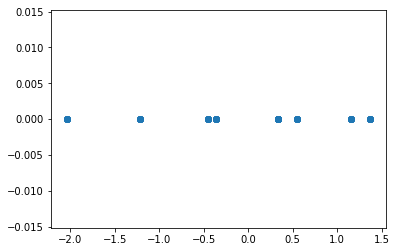
\includegraphics[width=0.4\textwidth]{SVW_0th_mode_Hamiltonian_Henon}
$k=3$
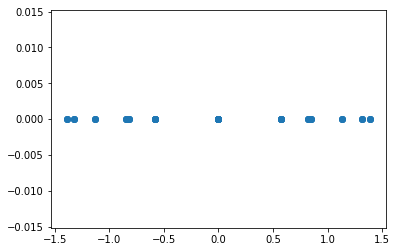
\includegraphics[width=0.4\textwidth]{SVW_3rd_mode_Hamiltonian_Henon}
\\
$k=1$
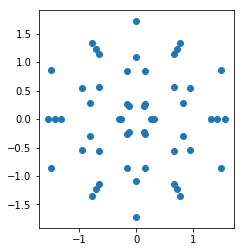
\includegraphics[width=0.4\textwidth]{SVW_1st_mode_Hamiltonian_Henon}
$k=2$
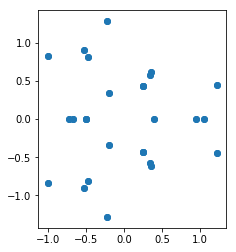
\includegraphics[width=0.4\textwidth]{SVW_2nd_mode_Hamiltonian_Henon}
\\
$k=5$
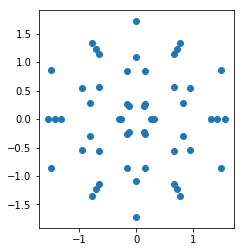
\includegraphics[width=0.4\textwidth]{SVW_5th_mode_Hamiltonian_Henon}
$k=4$
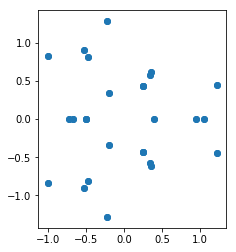
\includegraphics[width=0.4\textwidth]{SVW_4th_mode_Hamiltonian_Henon}
  \caption{
Hamiltonian \Henon\ \refeq{e_ar_pres}, $a=6$ {\lattstate}s of period
$\cl{}=6$, in the $\Cn{6}$ reciprocal lattice, $k=0,1,2,3,4,5$.
$k=0,3$ are purely real.
$k=5,4$ are the same as $k=1,2$, respectively, up to time reversal.
Compare with Han's \reffig{fig:HLCatMapLength6C6Fund}, for example.
}
\label{SVWHamHenFourier1}
\end{figure}


\item[2021-02-27 Sidney] Notes from Engel's course\rf{Engel11}.

If $G$ is a group and $X$ is a set, then a left group action of $G$ on $X$ is a binary function:
$$GX\rightarrow X$$
denoted
$$(g,x)\mapsto g\cdot x$$
Which satisfies the following two axioms:

1.$(gh)x=g(hx)$

2.$ex=x$

The set $X$ is called a left G-set. The group $G$ is said to act on $X$ on the left. When a group $G$ acts on a set $X$ the orbit of a point $x$ in $X$ is the set of elements of $X$ to which $x$ can be moved by the elements of $G$. The orbit of $x$ is denoted as $Gx$:
$$Gx=\lbrace g\cdot x| g\in G\rbrace$$
The properties of a group guarantee that the set of orbits of $X$ under the action of $G$ form a partition of $X$. The associated equivalence relation is $x~y$ if and only if there exists a $g$ in $G$ with $gx=y$. The orbits are then the equivalence classes under this relation, two elements $x$ and $y$ are equivalent if and only if their orbits are the same ie $Gx=Gy$. For every $x$ in $X$, we define the stabilizer subgroup of $x$ (also called the isotropy group or little group) as the set of all elements in $G$ that fix $x$:
$$G_x=\lbrace g\in G | g\cdot x=x\rbrace$$
In short: the orbit consists of all points that are equivalent under symmetry. And the stabilizer consists of all symmetries that leave a point invariant.

$\textbf{Definition 6}$: A point symmetry is a symmetry which leaves a point $x_0$ invariant: $\mathcal{T}(x_0)=x_0$

So, we can see that translations cannot be point symmetries, symmetries with finite order are point symmetries, symmetries with infinite order cannot be point symmetries.

$\textbf{Definition 7}$: A point group is a group of point symmetries which leave a common point $x_0$ invariant.

So, we can see that a point group is a finite subgroup of $O(3)$, this space of three dimensional orthogonal matrices.
$$\text{Note:  }O(3)=\lbrace A\in\R^{3\times3}:A^TA=1\rbrace$$
$$SO(3)=\lbrace A\in\R^{3\times3}:A^TA=1, det(A)=1$$

$\textbf{Definition 8:}$ Two subgroups $H_1$ and $H_2$ of a group $G$ are conjugated if there exists a $g\in G$, such that:
$$H_2=g^{-1}H_1g$$

$\textbf{Example}$: $G=O(3)$. Two point groups are conjugated, if there is a change of basis that maps them into each other.

$\textbf{Cyclic groups}$: $\Cn{1},\Cn{2},\Cn{3},...$ where $\Cn{n}$ consists of all rotations about a fixed point by multiples of $360/n$

$\textbf{Dihedral groups}$: $\Dn{1},\Dn{2},\Dn{3},\Dn{4},...$ where $\Dn{n}$
(of order $2n$) consists of the rotations in $\Cn{n}$ together with
reflections in $n$ axes that pass through the fixed point.

\item[2021-03-07 Predrag]
For the current project, we need to understand
$\Dn{n}$ symmetry: see
\HREF{http://chaosbook.org/projects/dingThesis.pdf\#exmple.2.9}
{Ding thesis example~2.9.}\\
pdflatex \emph{siminos/lyapunov/blog.tex}, read sect.~7.11.2
\emph{Factorization of $\Cn{n}$ and $\Dn{n}$}.

See also \refsect{sect:pw20210108}~{\em Pow wow 2021-01-08}.



\item[2021-03-07 Sidney]
% Here is my attempt to site the lecture notes that I have been drawing
% from: \rf{Engel11} it is very likely that I missed some important
% citation information, if I have I am truly sorry.
I shall now attempt
some of the exercises in Engel's\rf{Engel11}
\HREF{http://www-personal.umich.edu/~engelmm/lectures/ShortCourseSymmetry1.pdf}
{Point Groups} lecture.

\begin{itemize}
\item[Exercise 1]  \exerbox{exer:Engel11PG1}
\item[Exercise 3]  \exerbox{exer:Engel11PG3}
\end{itemize}

Determination of the point group of an object in space

1. Object linear: $\Cn{\infty v}$ or $\Dn{\infty h}$

2. High symmetry, non-axial: $T$, $T_h$, $T_d$, $O$, $O_h$, $I$, $I_h$

3. No rotation axis: $\Cn{1}$, $\Cn{i}$, $\Cn{s}$.

Carolyn's packings of small spheres on a big sphere

The point groups are for the sphere on the left: $\Cn{2v}$ because it has
3 axes that it can rotate $180^{\deg}$ around, and for each one it can
then perform a flip and remain unchanged, I am unsure about the second
sphere.
\item[2021-03-07 Predrag]
For the current project, it will suffices to focus on 1\dmn\ and 2\dmn\
crystals (wallpaper groups). Engel is a chemist, so 3\dmn\ symmetries
are the most important thing, but we are good enough keeping to 2 dimensions.

\item[2021-03-13 Sidney]
Here are my notes on Xiong Ding's example 2.9 and 2.8 in his thesis which is referenced above.
\begin{itemize}
\item[Example 2.8] Character table of dihedral group $D_n=C_{nv}$ n odd
$$D_n=\lbrace e, C_n,C_n^2,\cdots,C_n^{n-1},\shift,C_n\shift,\cdots , C^{n-1}_n\shift\rbrace$$
$D_n$ has n rotation elements and n reflections. Group elements satisfy
$C^i_nC^j_n\shift=C_n^j\shift C^{n-i}_n$, so $C^i_n$ and $C^{n-i}_n$ form a class.
Also,
$C_n^{n-i}C_n^{2i+j}\shift=C_n^j\shift C_n^{n-i}$ implies that
$C^j_n\shift$ and $C^{2i+j}_n\shift$
are in the same class. Therefore, there are only three different types of
classes:
\\
$\lbrace e \rbrace ,\lbrace C_n^k,C_n^{n-k}\rbrace,\lbrace
\shift,C_n\shift,\cdots,C_n^{n-1}\shift\rbrace$. The total number of
classes is $(n+3)/2$. In this case, there are 2 one dimensional
irreducible representations (symmetric $A_1$ and antisymmetric $A_2$)
and $(n-1)/2$ two-dimensional irreducible representations. In the
$j^{th}$ two-dimensional irreducible representation, class $\lbrace
e\rbrace$ has form $\begin{pmatrix}
1 & 0\\
0 & 1
\end{pmatrix}$, class $\lbrace C^k_n, C_n^{n-k}\rbrace$ has form $\begin{pmatrix}
\exp(\frac{i2\pi ki}{n}) & 0\\
0 & \exp(-\frac{i2\pi ki}{n})
\end{pmatrix}$, and class $\lbrace \shift,C_n\shift,\cdots,C_n^{n-1}\shift\rbrace$ has form  $\begin{pmatrix}
0 & 1\\
1 & 0
\end{pmatrix}$

Definition of Irreducible Representation (and Representation): Will be using the Dresselhaus lecture notes from 2002 downloaded from the \HREF{http://chaosbook.org/course1/Course2w14.html}{Chaosbook website}:

Representation: A representation of an abstract group is a substitution group (matrix group with square matrices) such that the substitution group is homomorphic (or isomorphic) to the abstract group. We assign a matrix $D(A)$ to each element $A$ of the abstract group such that $D(AB)=D(A)D(B)$.

Homomorphic/Isomorphic: Two groups are isomorphic or homomorphic if there exists a correspondence between their elements such that each
$$A\rightarrow\hat{A}$$
$$B\rightarrow\hat{B}$$
$$AB\rightarrow\hat{AB}$$
If the two groups have the same order, then they are isomorphic.

Irreducible Representation: If by one and the same equivalence transformation, all the matrices in the representation of a group can be made to acquire the same block form, then the representation is said to be reducible, otherwise it is irreducible. Thus, an irreducible representation cannot be expressed in terms of representations of lower dimensionality.

Aside: how to find a character table of a group. See \HREF{https://www.youtube.com/watch?v=mRoAvOHcsmo&ab_channel=TMPChem}{here} for the source, symbol $A$ denotes symmetric with $C_n$ so yields a 1 in the character table for all C. The subscripts 1, and 2 are symmetric (1) and antisymmetric (-1) respectively with respect to flips $\shift$. I am unsure about how the $E_j$ column got its entries, it looks like it was a trace of the matrix representations, but I don't know the rule for that.

\item[Q Sidney]
Conventionally, the irreps are the rows, and the symmetry operations are the columns, why are they transposed here?

\item[2021-03-18 Sidney]
A review of the Group theory from Chaosbook, especially the irreps, and character tables. The goal of this is so that I can actually understand the character tables presented in the examples of Xiong Ding's thesis.

\item[Q2 Sidney]
I am a little unsure about the statement in example 2.8 of Ding's thesis "in the jth two-dimensional irreducible representation class $\lbrace \shift , \shift C_n,\cdots ,\shift C_n^{n-1}\rbrace$ has the form $\begin{pmatrix}
0 & 1\\
1 & 0
\end{pmatrix}$. Shouldn't there a contribution from the rotation group $C_n$? This looks just like the inversion (reflection?) group $\shift$.

From Dresselhaus again.

The Unitary of Representations: This theorem which shows that in most physical cases, the elements of a group can be represented by unitary matrices.

Theorem: Every representation with matrices having non-vanishing determinants can be brought into unitary form by an equivalence transformation. Skipping writing out the nitty gritty of the proof, we can first form a hermitian matrix using the representations of the group. We can than take advantage of the fact that any Hermitian matrix can be diagonalized by a suitable unitary transformation. We can construct this by doing a similarity transformation with some $U$ from there we can redefine $\hat{\hat{A}}_x=d^{-1/2}U^{-1}A_xUd^{1/2}$ where $d$ is the diagonal matrix. We can then show that $\hat{\hat{A}}_x$ is unitary by simple calculation, thus we have proved the theorem.

We can use this theorem to prove Schur's Lemma which is: A matrix which commutes with all matrices of an irreducible representation is a constant matrix (a constant times the unit matrix). Therefore, if a non-constant commuting matrix exits, the representation is reducible.

Proof: Let $M$ be a matrix which commutes with all matrices of the representation $A_1,A_2,\cdots ,A_h$:
$$MA_x=A_xM$$
Take the adjoint of both sides:
$$A_x^{\dagger}M^{\dagger}=M^{\dagger}A^{\dagger}_x$$
From the Unitary Representations theorem, with no loss of generality we can assume that $A_x$ is unitary, so we can multiply on the left and right to obtain:
$$M^{\dagger}A_x=A_xM^{\dagger}$$
So, if M commutes with $A_x$ then so does $M^{\dagger}$.

\item[2021-03-22 Sidney]
I read through the rest of the proof, and I will continue Dresselhaus notes later, but now, I will review some \HREF{http://chaosbook.org/course1/Course2w13.html}{Chaosbook} material. I also looked at the decomposition of the cat map done by Predrag,
but I do not understand it enough to see if it works with the {\HenonMap}, so I will discuss in tomorrow's meeting. Anyway, here are notes for Week 13.

\begin{itemize}
\item[Video 1: Hard Work Builds Character]
Elementary examples of discrete groups: the character table characterizes
the finite group.

2-element group: $\lbrace e,g\rbrace$ $g^2=e$. $S_2,D_1,C_2,...$ used to
tile our space. Imagine butterfly, symmetry axis across the middle. Can
separate the space into two spaces
$\tilde{\mathcal{M}}\in\lbrace\tilde{x}\rbrace$ and
$\tilde{\mathcal{M}}_2=\lbrace -\tilde{x}\rbrace$ (top view of butterfly
space). On the side, it is just a line, half of the line can be the
fundamental domain, everything else is a copy of the fundamental domain.
(Order of the group is the number of elements in it). Think of scalar
functions defined on this domain $\rho(x)$. Can divide it into two
functions $\rho_1(\tilde{x})$ (defined on fundamental domain) and
$\rho_2=\rho(-\tilde{x})$. Can decompose this function into a vector of
functions evaluated on the fundamental domain, the vector will have a
length equal to the order of the group. Can write the original function
on the fundamental domain as
$\rho(\tilde{x})=\frac{1}{2}(\rho(\tilde{x})+\rho(-\tilde{x}))+\frac{1}{2}(\rho(\tilde{x})-\rho(-\tilde{x}))$
(decompose into symmetric, and antisymmetric components).
$\rho(\tilde{x})=\rho_+(\tilde{x})+\rho_-(\tilde{x})$.
$\rho_{\alpha}=\frac{1}{|G|}\sum_g\chi_{\alpha}(g)\rho$. Where $\chi$ is
the characters from the character table.

\item[Video 2: The Symmetry Group of a Propeller]
3 elements. $G=\lbrace e,g_2,g_3\rbrace$ $g^3=e$, rotation by $2\pi/3$
$C_3$ cyclic group with three elements. Can look at this as an abstract
group (no physical, or geometrical realization): $g_2=\omega$
$g_3=\omega^3$ $\omega^3=e$. Can write a multiplication table from these
relationships with the inverses, there is the identity along the
diagonal. Matrix representation: in 2D plane the identity is just the
unit matrix, and the other elements are just the rotation matrices.
    \end{itemize}
I shall end my notes here for today (it is getting late).
\end{itemize}


\item[2021-04-19 Sidney]
I have been working through the chapter~10
\toChaosBook{chapter.10} {problems}
and I'm pretty
confident with all but problem 10.2, could I possibly have a hint on
where to start?

\item[2021-03-07 Predrag]
I put all solutions that I have
\HREF{http://chaosbook.org/~predrag/old/2Sidney.pdf} {here}.
They are pretty incomplete.
If you have solutions that I do not have, or better / comparable solutions to those that
I do have, let me know.

\item[2021-04-24 Sidney]
Here I will attempt to derive the {\jacobianOrb}, so that I can
later find the eigenvalues and eigenvectors. I will start with
analytically finding {\lattstate}s, and eigen-things. We will see how
well that goes. First, the {\henlatt} is $x_{n+1}+ax_n^2+x_{n-1}-1=0$
this was drawn from the beginning of \refchap{c-Henon}~{\em \Henlatt}.
Following the formalism of the CL18 paper, I can rewrite the map as
$\shift+2a{\mathbb{X}}+\shift^{-1}-I=0$ where the $2$ has come from the fact that
finding the {\jacobianOrb} is in effect taking a derivative, now the
{\jacobianOrb} is
\\~[{\bf 2021-05-01 Sidney}: \emph{this has wrong entries
on the diagonal, \refeq{SVWorbitJac}, \refeq{Henlatt-orbitJac} is the
correct formula.}]
$$\jMorb=\shift+2a{\mathbb{X}}+\shift^{-1}=\begin{bmatrix}
2ax_n & 1 & 0 & 0 & \dots & 0 & 1\\
1 & 2ax_n & 1 & 0 & \dots & 0 & 0\\
0 & 1 & 2ax_n & 1 & \dots & 0 & 0\\
\vdots & \vdots & \vdots & \vdots & \ddots & \vdots & \vdots\\
0 & 0 & \dots & \dots & \dots & 2ax_n & 1\\
1 & 0 & \dots & \dots & \dots & 1 & 2ax_n
\end{bmatrix}\,,$$
where the ones on the upper right and lower left corners, are a result of
the periodic boundary conditions. The goal is to adapt this so that we
can apply the time reversal boundary conditions, and thus construct
time-symmetric {\lattstate}s.

\item[2021-05-01 Sidney]
Here is the correct {\jacobianOrb} (in the above I made a mistake):
\bea
\jMorb &=&\Refl+2a{\mathbb{X}}+\Refl^{-1}
    \continue
            &=&
\begin{bmatrix}
2ax_0 & 1 & 0 & 0 & \dots & 0 & 1\\
1 & 2ax_1 & 1 & 0 & \dots & 0 & 0\\
0 & 1 & 2ax_2 & 1 & \dots & 0 & 0\\
\vdots & \vdots & \vdots & \vdots & \ddots & \vdots & \vdots\\
0 & 0 & \dots & \dots & \dots & 2ax_{n-2} & 1\\
1 & 0 & \dots & \dots & \dots & 1 & 2ax_{n-1}
\end{bmatrix}
\label{SVWorbitJac}
\eea
% This of course means that the calculations I did with the previous matrix
% are useless. I shall redo them, maybe code it this time. As well, tomorrow,
I'll look at (and try to understand) the proof of the Hill's
formula.

\item[2021-05-05 Predrag]
Please modify your code so you are computing the (rescaled) {\henlatt}
\refeq{Henlatt-2-step}, {\jacobianOrb} \refeq{Henlatt-orbitJac}.

\item[2021-05-05 Sidney]
I shall modify my code to do that, first, I will look at the rescaled
{\henlatt} \refeq{Henlatt-2-step}. Just for my own satisfaction, I shall
rederive \refeq{Henlatt-2-step} and \refeq{Henlatt-orbitJac}. The
Hamiltonian \HenonMap\ is given by
$$x_{n+1}=1-ax_n^2-x_{n-1}$$
We note that an n-step recurrence relation is the discrete analogue to an
order-n differential equation. We can now introduce the change of
variables $\phi_n\equiv ax_n$ this turns our map into:
$$\frac{1}{a}\phi_{n+1}=1-\frac{1}{a}\phi^2_n-\frac{1}{a}\phi_{n-1}$$
Rearranging, we get
\beq
a=\phi_{n+1}+\phi^2_n+\phi_{n-1}
\,.
\ee{SVWhenlatt-2-step}
The derivative of this map yields its {\jacobianOrb}:
$$\jMorb_p=\shift+2{\mathbb{X}}+\shift^{-1}$$
Thus, we have rederived \refeq{Henlatt-2-step} and
\refeq{Henlatt-orbitJac}. I can now put it into my code. I am currently
trying to understand the derivation of:
\[
\hat{\jMorb}_p =
\left[
\begin{array}{ccccc}
 {\unit} &  &  &  & -\jMps(\field_0) \\
 -\jMps(\field_1) & {\unit} &  &  &  \\
  & \ddots & \ddots &  &  \\
  &  & -\jMps(\field_{n-2}) & {\unit} &  \\
  &  &  & -\jMps(\field_{n-1}) & {\unit} \\
\end{array}
\right] \, ,
\]
Any hints would be much appreciated.

\item[2021-05-10 Predrag]
It's all in the blog,  and the \emph{siminos} repo. But why don't you go
back where you started, and reread CL18\rf{CL18}:

\HREF{http://chaosbook.org/~predrag/papers/CL18.pdf\#subsection.1.5}
{sect.~1.5} {\em  Stability of an orbit vs.  its time-evolution stability}

\HREF{http://chaosbook.org/~predrag/papers/CL18.pdf\#appendix.C}
{appendix~C} {\em Spatiotemporal stability}

\item[2021-05-10 Predrag]
One thing you can maybe help Han and me with; we find the block matrix
formulation of \refsect{sect:catlattHill}~{\em \catLatt\ Hill's formula}
quite reader-unfriendly. I like the latest version,
\refsect{sect:HenonHillHan}~{\em Han's  \HenonMap\ Hill's formula} better.
Any suggestions how to make this easier to read are welcome!

\item[2021-05-06 Matt to Sidney]

It's not clear to me what you need help with, but the origin of the
derivation of the aforementioned matrix is the Jacobian of a multipoint
shooting method
(see \toChaosBook{section.16.2} {sec.~16.2} {\em  Multipoint shooting method}
and
\toChaosBook{exmple.16.2} {example~16.2}%
)
vector $x_n - f(x_{n-1}),\quad n\in {0, ..., N}$ (indices
may be off depending on how matrix is ordered), which finds cycles of
length $n$ by solving a system of single steps.
If the vector equals 0 then this means that we have found a cycle/orbit as we have found a set of points which is closed under
evolution (we can take $N$ steps and return to our original position, starting from any of the $N$ points defining the cycle).
The actual matrix, as with all Jacobians, tells us how the tangent space evolves. In terms of the multipoint shooting,
this is the combination of $N$ single step Jacobians. If you are on the cycle (i.e. no deviations, or components in the tangent space)
which evolve other than the velocity, which is mapped into the velocity at the new point.
This is a quick and dirty explanation which is probably over simplifying, but
the near-tautological explanation is: if you're on the cycle, then you don't get pushed away from the cycle due to your deviation from the cycle.

\textbf{tl;dr} It's the Jacobian of the multipoint shooting equation $x_n - f^t(x_{n-1})$.

\item[2021-05-10 Predrag]
Talking about multishooting, the material around eq.~\refeq{errorVecsTrevers}
might be worth revisiting.

\item[2021-05-09 Sidney]
Thank you Matt, it makes sense now, given the definition of the single
step Jacobian it just sort of pops out. So, at this point I know how to
get both the traditional {\jacobianOrb} (which I am currently working on
coding in) and the {\jacobianOrb} in terms of the single step Jacobian
(which I also know how to derive).

\item[2021-05-09 Sidney]
At this point, I am trying to
understand the block matrix form that can be generated by applying a
permutation matrix defined by the circular Kronecker delta. What I do not
understand, is:

What is the difference between the circular Kronecker delta, and the regular one?

\item[2021-05-10 Predrag]
Regular one is defined on $\integers$ (no restrictions), the circular one
on \Cn{\cl{}} (periodic chain, so $\mod \cl{}$).
(Re)read \toChaosBook{section.X.3}
% equation.X.3.25}
{appendix~X.3} {\em Discrete Fourier transforms}.

\item[2021-05-09 Sidney]
And I am also having difficulty deriving the appropriate permutation
matrix. I want to try turning the two-cycle {\jacobianOrb} (in terms of
single-step Jacobians) into the block matrix form. The following is my
(incorrect) derivation of the 4x4 permutation matrix. I have assumed that
when the index for the circular Kronecker delta reads something like
$4,j$ it is equivalent to $0,j$, as that would be equivalent to going to
the end of the columns (index $j$) and then starting back at the
beginning. By doing this I get: P is a $[2n\times 2n]$ permutation
matrix. Defined through the circular Kronecker delta:
$P_{k,j}=\delta_{2k-1,j}$, for a periodic orbit of length $n=2$ P is
$$P=\left[\begin{matrix}
1 & 0 & 0 & 0\\
0 & 0 & 1 & 0\\
1 & 0 & 0 & 0\\
0 & 0 & 1 & 0
\end{matrix}\right]$$
(This is wrong)

What did I do wrong?

\item[2021-05-10 Predrag]
By `permutation matrix' you mean the one-step cyclic permutation
$\shift$, or the shift matrix \refeq{shiftMatrix}? The circular
Kronecker delta is just the $[\cl{}\times\cl{}]$  identity matrix. I
leave it to Han and you to figure out what went wrong :)

\item[2021-05-13 Han]
My Kronecker delta representation was wrong... \refeq{HLHillDetPermutation}
should be correct. I don't have a more compact way to write this permutation
matrix. The permutation matrix for $n=2$ is:
\[
\left[
\begin{array}{cccc}
 1 & 0 & 0 & 0 \\
 0 & 0 & 1 & 0 \\
 0 & 1 & 0 & 0 \\
 0 & 0 & 0 & 1 \\
\end{array}
\right]
\, .
\]

\item[2021-05-10 Predrag]
To everybody - always number sites of length-$\cl{}$ periodic chains
(necklaces) as
\[\{0,1,2,\cdots,\cl{}-1\}\,,\]
otherwise discrete Fourier transforms will go awkward on you.

\item[2021-05-10 Predrag]
Regarding \refsect{e:CenterOfMass} {\em ``Center of mass'' puzzle}:

Relevant Gallas papers are all in ChaosBook.org/library, for example
\CBlibrary{EG05}, with their names (always!) given by their BibTeX ID.

Predrag's unpublished 2004 drafts and calculations can be accessed by
clicking on the link given there:

\wwwcb{/projects/revHenon}

There is no need to  look at old drafts of papers, as the most of the
relevant stuff is already included in that section, but the link
includes some data files, orbit plots and programs that might be useful
to Sidney as crosschecks on his calculations.

\item[2021-05-12 Sidney]
Here are some notes from the last meeting: Any matrix can be written as a sum of projections into the different eigendirections. An anti-diagonal matrix, as well as the anti-diagonal matrix multiplied by sigma and its powers give the reflection matrix, and the reflection matrix across all axes.
\item[Q] What are these axes?
A reflection matrix has two eigenvalues $\pm 1$ (corresponding to either
the symmetric, or antisymmetric subspace), and a projection operator can
be constructed by subtracting out the opposite of the subspace you want
to project onto. This projection operator can be applied to the left of
the {\jacobianOrb} to project it onto either the symmetric, or
antisymmetric space. In this way, the {\jacobianOrb} can be written as
$\jMorb=\jMorb_-+\jMorb_+$, it is worth noting that
$\det(A+B)\neq \det(A)+\det(B)$. In the case of a linear map (where the
fundamental fact still applies) the determinant of $\jMorb_{\pm}$
counts the number of time symmetric/antisymmetric orbits. Note that we
need to apply the time symmetric boundary conditions in order to enforce
time symmetric orbits.
\item[Q2] Is this last statement correct?
I have now updated my code to work with the scaled {\HenonMap}. Actually, I just did the lazy thing of dividing all values in all orbits by $a$. I also added a function to generate the (scaled) {\jacobianOrb}, and I tried calculating its eigenvalues and vectors, it all seems to work, but I'm really not sure what I should be seeing for eigenvalues and vectors, I will paste my code below (I will past all of it, but it's mostly the same as before, just with a little added on the end):
There is probably some extra code in there that just isn't being used, but hey, it's a work in progress.
Update 2021-05-17: I have added this code to the williams/relax folder in the subversion, so I have now deleted the code here.

\item[2021-05-13 Sidney]
With Han's help I was able to see the permutation matrix, and I was able
to reproduce the Hill's formula "proof" for the specific case of n=2 (I
use quotation marks because I only proved it for one case, and not all
cases) I will probably keep thinking about how to generalize it, but I
now feel better about applying Hill's formula to my {\jacobianOrb}. I
have been trying to work through the algebra with the reflection, and the
corresponding projection matrices described in Han's most recent blog
post. I understand qualitatively what's happening, effectively the
projection operator is just the reflection operator with one of the
eigenspaces subtracted out, with an additional weight that forces the
identity $\mathbb{1}=\sum_iP_{A_i}$, this is a formula for a generic
matrix. I cannot find anywhere in lectures, or textbooks where this is
formalized, so I am not sure how the weights are constructed, but I'll
keep looking at it.

\item[2021-05-15 Matt]
I'll put a couple of responses here to hopefully help Sidney out.
Response to questions in 2021-05-12 Sidney.
It seems like the questions are with respect to the proceeding sentences but they are in different paragraphs so it is unclear to me if that is what you meant.

\textbf{Q What are these axes?} Is the question with respect to a specific system or just in general? If we're talking about reflection in $D$ dimensional euclidean space then we can reflect over any $D-1$ dimensional hyperplane, so I'm assuming it's talking about reflection where the eigenvectors are the normal vectors to these planes, so the hyperplane which is normal to each eigenvector can define a reflection so maybe this is what you're referring to?

\textbf{Q2 Is this last statement correct?} What is "the last statement"? The last statement before the question, the last statement of the previous paragraph...? Is it the following?
\begin{quote}
Note that we need to apply the time symmetric boundary condi-
tions in order to enforce time symmetric orbits
\end{quote}
To ensure that you get a time symmetric orbit then yes you have to impose boundary conditions which constrain you to that subspace. The unconstrained method (if variational in formulation) could possibly find these orbits, but there would be no guarantee.

Response to 2021-05-13 Sidney.
\begin{quote}
I understand qualitatively what’s happening, effectively the projection operator is just the reflection operator with one of
the eigenspaces subtracted out, with an additional weight that forces the
identity $\mathbb{I} = \sum_i P_{A_i}$, this is a formula for a generic matrix. I cannot find
anywhere in lectures, or textbooks where this is formalized, so I am not
sure how the weights are constructed, but I’ll keep looking at it.
\end{quote}
Where "this" is formalized: The "weights" are simply normalization coefficients. The sum of the projection operators equaling the identity essentially says that the "full" space can be decomposed into projection subspaces, each of which has its own projection operator. I.e.
each subspace is a component of the full space. Predrag formalizes
the projection operators \textit{a lot}; especially in his group theory stuff which this is directly related to.

For a reflection operator we can decompose
$$\sum P_{\pm} = \frac{1}{2}(\mathbb{I}\pm R) = 1/2 (\mathbb{I} + \mathbb{I} + R - R)
               = 1/2 (2\mathbb{I}) = \mathbb{I}\,.$$

For a symmetry subspace that can be broken into 4 subspaces, the normalization would be $1/4$, etc.

\item[2021-05-23 Sidney]
Thank you to Matt for the explanation, I also have now attended the group theory lecture on projection operators (I've actually been thinking about this a good bit, but taking the time to condense my thoughts onto my blog is not one of my strong suits). Anyway, the projection operator formalism for matrices can be derived from the Hamilton-Cayley theorem:
$$\prod_i\left(\mathbb{M}-\lambda_i\mathbb{I}\right)=0$$
In words, this is just the statement that a matrix satisfies its own characteristic equation. However, if we take one element out of the product, the RHS will no longer be zero:
$$\prod_{i\neq j}\left(M-\lambda_i\mathbb{I}\right)=\prod_{i\neq j}\left(\lambda_j-\lambda_i\right)\textbf{e}_i$$
We can rearrange to get:
$$\mathbb{P}_j=\prod_{i\neq j}\frac{\mathbb{M}-\lambda_i\mathbb{I}}{\lambda_j-\lambda_i}$$
Which is the definition of the projection operators that Han used, I was also
able to reproduce his results. I also found out an issue with my code for
finding time-reversal symmetric orbits. I was not taking into account
permutations, but that is an easy fix, that I hope to fix quickly.

When I have, I can create a bank of orbits appropriate to use with the
{\jacobianOrb} projected into the symmetric subspace using projection
operators, I know how to construct this both by hand, and by code, I just
need to implement it. I also need to go through chapter 15 in Chaosbook, as
it gives good visualization of what the Hamiltonian {\HenonMap} does. I will
add my notes here when I have a chance, hopefully tonight, or tomorrow. I
also think that I should explore the volume of the parallelpiped represented
by the \jacobianOrb. I could probably use a package for that, but what I'll
most likely do is just use the fact that the determinant of a matrix is just
the product of its eigenvalues:
$$\det{A}=\prod_i\lambda_i$$
Then take the absolute value. I can then check the volumes generated by
different orbits.

\item[2021-05-26 Sidney]
I reviewed the \catlatt\ derivation to see if I could extend the idea to the
{\HenonMap}, I think I have.

If we enforce the following restrictions, we can qualitatively derive the
spatiotemporal {\HenonMap}:
\begin{itemize}
\item Each site couples to its nearest neighbors
\item Spatial and temporal coupling is of the same strength
\item Invariant under spatial translations
\item Invariant under spatial reflections
\item Invariant under space time exchange
\end{itemize}
With these conditions our {\henlatt}
\refeq{Henlatt-2-step}, \refeq{SVWhenlatt-2-step}
$$a=\phi_{t+1}+\phi_t^2+\phi_t$$
generalizes to my proposal for the {\henSTlatt}
\beq
\phi_{n,t+1}+\phi_{n,t-1}+2\phi_{n,t}^2+\phi_{n+1,t}+\phi_{n-1,t} = a
\,.
\ee{SVWhenSTlatt}
The factor of two comes from adding together two \HenonMap s (one spatial and
one temporal), following the derivation of the \catlatt. I need to try to
read Gutkin and Osipov\rf{GutOsi15} \arXiv{1503.02676} to get a better
idea of the derivation.

\item[2021-05-28 Predrag] I doubt you will find it in Gutkin and
    Osipov\rf{GutOsi15} - if you do, cite their words in detail here. The
    above argument is mine, from Gutkin \etal\rf{GHJSC16} and CL18 (kittens/ folder
    in this repository).

\item[2021-05-28 Predrag]
Your {\henSTlatt} \refeq{SVWhenSTlatt} looks OK to me, except maybe adding the
maps for each direction of a $d$\dmn\ lattice results in $da$ on the RHS?
In the spirit of
\HREF{http://chaosbook.org/~predrag/papers/CL18.pdf\#equation.3.80}
{eq.~(80)} in \texttt{CL18.pdf}?

How does your {\henSTlatt} compare to Politi and Torcini\rf{PolTor92},
\refsect{sect:PolTor92}~{Periodic orbits in coupled {H{\'e}non} maps}?

\item[2021-05-27 Sidney]
Here is my attempt at looking at the eigenvalues, eigenvectors, and the
determinants of the {\jacobianOrb}. My {\jacobianOrb} constructor only
works with orbits of length 3 and above, this is because is row has three
values in it that permute, and I'm not sure how to scale it down, will
discuss this at the next meeting. I cannot tell anything about the eigen
stuff so far, it seems almost random, however, the determinant values are
each approaching an integer value, so maybe that is something.

Note: I removed the table here because it was wrong

I will hopefully rearrange some of these tables to group them by orbit in a
later post, but for now, here is the "raw" data, let me know if anything
appears.

\item[2021-05-31 Sidney]
I'm not sure why, but the large table with all of the eigenvalues does
not appear in the pdf version of the blog. I am not sure how to fix that,
if anyone could let me know, that would be great. I still need to put it
into a more readable format anyway. I also looked at
\HREF{http://chaosbook.org/~predrag/papers/CL18.pdf\#equation.3.80}
{eq.~(80)} in \texttt{CL18.pdf}, and it is the reason that I did not have
$d*a$ on the RHS, the form of the spatiotemporal cat
\HREF{http://chaosbook.org/~predrag/papers/CL18.pdf\#equation.3.79}
{eq.~(79)}, has only $\textbf{M}$ not $2\textbf{M}$, which it would have
if both sides were added (right?), I need to read up on the coupled maps,
that will be something I do next (along with the better tables).

%\item[2021-06-03 Sidney]
%I've removed the big table because it is hard to read, and because we are in
%particular really worried about the period-4 eigenvalues:
%\bea
%1000 && ~2.06999154, -1.93402429, ~0.13608276, ~0.00011550,
%\continue
%1110 && -2.07703728, ~1.94208935, -0.13608276, -0.00113482.
%\continue
%1100 && ~2.00921679, -2.00921678, ~0.00921679,  -0.00921678
%\label{OrbJac4eigvsWrong}
%\eea
%
%\item[2021-06-04 Predrag]
%    By signs, `1100' looks like a repeat of `10', but that is surely not
%    true. Have a look at \reffig{COMcycles}\,(b).
%`1110' looks like the negative of `1000' (I've presumably gotten zeros
%wrong in the smallest eigenvalue), which might be a good thing: maybe
%time inversion amounts to $0\leftrightarrow1$ and eigenvalue
%$\leftrightarrow$ -eigenvalue? I do not think that the eigenvalues
%calculation is inaccurate, as the branches of the unstable manifold are
%curved, the cycle stabilities are different.

    That would also say that `1100' is symmetric under time inversion.

\item[2021-06-03 Sidney]
% We are concerned that some of eigenvalues in \refeq{OrbJac4eigvsWrong} are so
% small.
I want to try to take advantage of Hill's formula:
\beq
\Det(\jMorb_p) = \det(\id-\jMat_p)
               = (1-\ExpaEig_p)\left(1-\frac{1}{\ExpaEig_p}\right)
               = 2-\ExpaEig_p-1/\ExpaEig_p
\,.
\ee{SVWhillFrml}
So, I need to calculate the eigenvalues for the scaled time-step
{\jacobianM}, but first I need to find the form of the scaled time-step
{\HenonMap} \refeq{eq2.1a}
\bea
    x_{n+1}&=&1-ax^2_n+b y_n
        \continue
    y_{n+1}&=& x_n
\label{eq2.1a}
\eea
We scale
$x\rightarrow\frac{1}{a}\field$, $y\rightarrow\frac{1}{a}\varphi$,
and the {\HenonMap} becomes:
\bea
    \field_{n+1}&=&a-\field_n^2+b \varphi_n
        \continue
    \varphi_{n+1}&=& \field_n
\label{Gallas:eq2.1a}
\eea
%$$\field_{n+1}=a-\field_n^2+\frac{b}{a}\varphi_n$$ PC 2021-06-04: wrong
%$$\varphi_{n+1}=\field_n$$
Temporal stability of the $n$th iterate of the Hamiltonian {\HenonMap} is
\index{Henon@H\'enon map!stability}
\PC{2021-06-04}{Was
$$\begin{bmatrix}
-2\field_n & \frac{b}{a}\\
1 & 0
\end{bmatrix}$$
The correct form is \refeq{COM:e_her}. Hence, with Sidney's ``scaled
Jacobian,'' the four cycle Floquet multiplies were all wrong.
}
\beq
\monodromy^n(\field_0) = \prod_{m=n}^{1}
          \MatrixII{-2 \field_m}{ -1 }
                   {1}  {0}
\,,\qquad \field_m = f^{m}_1 (\field_0,\varphi_0)
\,.
\ee{SVW:e_her}
It is very important to understand the Floquet multipliers are invariant under
all smooth coordinate changes, see
\toChaosBook{section.5.4}{sect.~5.4}, so they are not affected by this rescaling..
When we find the eigenvalues of this matrix
they give contracting and expanding, we are interested in the expanding
stability multiplier.
There are three period 4 {\orbit}s: 1110, 1100, 1000, they have the following
expanding Floquet multipliers:
% associated with the scaled time-step Jacobian:
%\begin{table}[ht]
%\caption{Eigenvalues for 4 Cycles} % title of Table
%\centering % used for centering table
%\begin{tabular}{c c c} % centered columns (4 columns)
%\hline\hline %inserts double horizontal lines
%Orbit : & 1110 & 1100 & 1000 \\ [0.5ex] % inserts table
%%heading
%\hline % inserts single horizontal line
%| & 0.99996854+0.00793269j & 0.98165216 & 0.99968853+0.02495685j\\ % inserting body of the table
%| & 0.99996854-0.00793269j & 1.01869078 & 0.99968853-0.02495685j\\[1ex] % [1ex] adds vertical space
%\hline %inserts single line
%\end{tabular}
%\label{table:eigen4} % is used to refer this table in the text
%\end{table}
%As can be seen, 1110 and 1000 do not have expanding eigenvalues, which kinda stops me in my tracks.

\item[2021-06-04 Predrag]
I do not seem to have handy list of the Hamiltonian $a=6$ {\HenonMap} Floquet
multipliers. Floquet exponents for many $a=1.4,b=0.3$ {\orbit}s are
listed in \toChaosBook{table.caption.560} {table 34.2}. I believe that
\refsect{sect:HenonHillHan}~{\em Han's  \HenonMap\ Hill's formula} also
applies to the dissipative case, might be worth by repeating the
derivation with $b\neq-1$, or at least checking it for a few short \po s.

\item[2021-06-11 Sidney]
I have read some of Wen's 2014 project \wwwcb{/projects/Wen14.pdf}, I
should take some notes and put them here.
%I am still baffled by my error, as has been explained in
%several emails, I put the incorrect "scaled Jacobian" here (in this blog)
%but the correct one in my code. Despite this, the eigenvalues still
%change when I change from regular to scaled coordinates (this shouldn't
%happen, as explained in \toChaosBook{section.5.4}{sect.~5.4}).
%Update: I am made a ridiculous mistake, I said in my code that
%$\phi=\frac{x}{a}$, even though the change of coordinates was
%$x=\frac{1}{a}\phi$, I corrected this, and now the eigenvalues are
%working out correctly, I shall now redo the above analysis for the four
%cycles that was incorrect before.

\item[2021-06-11 Sidney]
The {\HillDet} should equal $2-\ExpaEig_p-{1}/{\ExpaEig_p}$ by Hill's formula
\refeq{SVWhillFrml}, where $\ExpaEig_p$ is the expanding eigenvalue of the
time-step Jacobian for that orbit, see \reftab{tab:det4}.
%None of these match the values for the {\HillDet}, but as mentioned
%above, I was using the wrong definition of $\phi$ and that would
%obviously make the rest of the values wrong,
%I shall remove the above table of {\HillDet}s
%% {\jacobianOrb} determinants
%in the next blog update.

\item[2021-06-11, 2021-06-23 Sidney]
\refTab{tab:orbitdet} lists the {\HillDet}s
computed from the {\jacobianOrbs}.
%  using the correct scaled orbits:
Comparing with \reftab{tab:det4} period-4 {\HillDet}s, we see that the
Hill's formula \refeq{SVWhillFrml} is satisfied to high precision.
% I shall check more thoroughly later, and also recompute the period-4
% eigenvalues \refeq{OrbJac4eigvs}.

\item[2021-06-12 Predrag]
It looks like you now have the correct {\HillDet}s. Their numbers agree with
\toChaosBook{table.caption.358}{Table 18.1}; there are 6 period-5
orbits, and 9 period-6
orbits. The period-6 itineraries are not yet correctly assigned, fix that.
The ones with even \#'s of `1's are presumably the positive ones.

\item[2021-06-12 Sidney]
I shall fix the itineraries for 6 cycles, and I'll add the itineraries of
the other, shorter cycles later. Some were correct, and the negative
determinants were in fact the odd number of 1s.

\item[2021-06-13 Predrag]
Do include fixed points and the period 2 in \reftab{tab:orbitdet};
might be helpful for understanding magnitudes of longer period {\HillDet}s.

\item[2021-06-13 Predrag to Han and Sidney]
If you think of the \HenonMap\ as a fattened parabola, then 0 fixed point
has large positive slope (4 for the Ulam map), and 1 fixed point has
small negative slope (-2 for the Ulam map). This explains the magnitudes,
and should also determine the signs of {\HillDet}s in \reftab{tab:orbitdet}.

However, either there is a - sign specific to Sidney's definition of the
\Henon\ {\jacobianOrb}, or Han and Predrag have to redefine both
\templatt\ and \henlatt\ {\jacobianOrb}, so we do not pick up an
extraneous `-' sign for odd period {\lattstate}s.

See also \refeq{Pozrikidis14(1.1.3)}.

Fixing this is not essential, as we use only the absolute values of
determinants in \po\ formulas.

\item[2021-06-13 Sidney]
In the 2014 project paper by Haoran Wen, it is stated that for a range of a
and b, the \HenonMap\ is “structurally stable” and that means that the
transport properties of the system have a smooth dependence on the
parameters. And then it states that the lack of structural stability will
result in the creation and destruction of infinitely many periodic orbits for
any parameter change. Does that mean that a structurally stable system has
relatively few bifurcations?

\item[2021-06-13 Predrag]
It's a long story, starting with a wrong conjecture by Smale, but the answer
is NO bifurcations for open intervals of system parameter values. Tends to be
possible only for repellers, that is why you are working with \Henon\ $a>6$ which
has all possible binary symbolic dynamics cycles, and no bifurcations as you
increase the parameter a.

Cat map has a finite grammar (is a "generating partition") for precisely
s=\emph{integer} >2, but change s to an open interval of real values around
-let's say- s=3, and
infinity of cycle get created and destroyed for any finite change in s.

\item[2021-06-13 Sidney]
So, at a=6 we achieve all binary symbolic dynamics, and anything more than
that we still have all binary symbols? No creation or destruction? Is there a
proof for this in the blog or somewhere else easily linkable to, that
wouldn't take me days to digest?

\item[2021-06-13 Predrag]
No, not $a=6$ - that's just the closest integer value.
\toChaosBook{section.15.2}{sect.~15.2 {\em Horseshoes}} explains it,
and -for example- Endler and Gallas\rf{EG05} say ``This classification is
independent of the control parametera. Orbits   are   specially   interesting
for $a>5.69931\dots$, since beyond this value there is a complete Smale
horseshoe\rf{HamSteDuMei99} and all orbits are real.''


\item[2021-06-14 Sidney]
blogCats is being weird for me, it is only showing the most recently added
parts, plus the table of contents, so right now when I build it, it only
gives the dihedral groups chapter, even though all the include commands are
not commented out.

\item[2021-06-14 Predrag]
In \texttt{inclOnlyCats.tex} the uncommented line was
\begin{verbatim}
\includeonly{chapter/groups}
\end{verbatim}
so \texttt{blogCats.tex} was doing what it should.

\item[2021-06-14 Sidney to Predrag and Han]
I am having trouble defining the {\jacobianOrb}  for orbit length 1 and 2,
this is because my code is designed to have a minimum width of 3 for the
matrix, because there needs to be the terms for
$\phi_{n+1},\phi_{n-1},\phi_{n}$, and I am not sure how to do that for 1 and
2 orbit lengths, should I just have the orbit repeat?

\item[2021-06-14 Predrag]
The fixed points and period-2 lattices you can evaluate by hand, I believe.
CL18 \HREF{http://chaosbook.org/~predrag/papers/CL18.pdf\#subsection.1.4}
{sect.~1.4} {\em  Fundamental fact} and
\HREF{http://chaosbook.org/~predrag/papers/CL18.pdf\#subsection.2.4}
{sect.~2.4} {\em  Fundamental fact}
evaluate the period-2 lattice {\jacobianOrbs}. If you understand how
\refeq{HLHessianLenth1},
\refeq{HLHessianLenth2}, and
CL18 \HREF{http://chaosbook.org/~predrag/papers/CL18.pdf\#equation.3.103}
{(103)} were derived, you will understand all such special cases.

\item[2021-06-14 Sidney to Predrag and Han]
Is 6 digits of
accuracy good enough? Is there a different method I should use? I am using
the one from
\toChaosBook{chapter.7}
{chapter 7} {\em Fixed points}
(the link is right here, I'll use that style of referencing in the future).
%, my next
%mini project for this blog is to create an index for links so if I repeatedly
%reference something, I can just draw from that)

\item[2021-06-18 Sidney to Predrag and Han]
I am trying to reproduce the projection operator analysis for \Dn{6}
symmetric {\lattstate}s and I am not really sure how to do that, which of
Han's posts talks about the {\lattstate}s? As well, doesn't the projection
analysis apply for \Dn{\cl{}} in general, not just specific {\lattstate}s?

% \item[2021-06-18 Predrag]

\item[2021-06-19 Sidney to Predrag and Han]
I tried to read Endler and Gallas\rf{EG05a}
\HREF{http://www.inaesp.org/PublicJG/conjugacy_classes_PLA_356_1_2006.pdf}
{2006 paper}
(not the Endler and Gallas paper\rf{EG05} that Predrag mentioned)
because Predrag said that it explained two period 3, one period 4, and two
period 6 values in my \reftab{tab:orbitdet}, but I
am not quite sure how the authors are getting their P polynomials, or their S
polynomials, specifically, I am not sure where the a value comes in, because
when I just try to expand their eq.~(3) and regroup it into eq.~(6), I could
not, so I am very confused. What obvious thing am I missing?

\item[2021-06-19 Predrag]
To ``expand their eq.~(3) and regroup it into eq.~(6)'' you need to know
analytically all period-4 periodic points, do you know them? They claim that
``the solution of this problem is trivial because \refref{EndGal02} contains
the solution for arbitrary $a$ and $b$.''

However, I was referring to the Endler and Gallas\rf{EG05} Table 1.
%period-3 orbits involve $\sqrt{7}=2.645751311$
The invariant quantity that
they associate with a \po\ is the orbital sum \refeq{COMdef}, the sum over
the periodic points, while the {\HillDet} involves various sums over values
of fields raised to various powers.
You will immediately note that the cases that have integer orbit sums
correspond to your integer-valued {\HillDet}s.
They had no reason to think of
{\HillDet}s, so that would be a major reworking of their paper(s); I do not
think you want to do that.

\item[2021-06-20 Sidney to Predrag and Han]
Oops
\vspace{3mm}

I agree that a major reworking is probably not in the cards, I will go back
to trying to understand {\jacobianOrbs} for the fixed point, and period 2
orbits. Endler and Gallas\rf{EG05a,EndGal02} look
exceptionally cool, I'll give them a whirl.

\item[2021-06-23 Sidney]
I worked through both Endler and Gallas papers\rf{EG05a,EndGal02}, as much as I could.
Here is what I came up with: in \refref{EG05a} the two important equations are
$P_k(x)$ and $S_k(\sigma)$, where $S_k(\sigma)$ is found through manipulating
the (scaled) {\HenonMap} and $\sigma$ is the sum of all points in the cycle,
$P_k(x)$ is defined as
\[P_k=\prod_{\ell=1}^k(x-x_\ell)\,,\]
where $x_l$ is the $\ell$th orbit point. The algorithm is simple: construct
$P_k(x)$ by expanding the product and putting each coefficient in terms of
$\sigma$, then use $S_k(\sigma)=0$ to determine how many unique orbits of
length k and 2. what values $\sigma$ can take, then combine with $P_k(x)$ to
solve for each orbit point. I will work two examples, first an orbit of
length 1:
$$\sigma=x_1$$
$$P_1=x-\sigma$$
$$x_{t+1}=a-x_t^2-x_{t-1}=x_1=a-x_1^2-x_1$$
Or
$$2\sigma+\sigma^2-a=0=S_1(\sigma)$$
As this is a quadratic equation, we know that there are two different fixed
points, and we can solve for them directly via $S_1(\sigma)=0$, now for an
orbit of length 2:

It is useful to first state that $a=2x_2+x_1^2=2x_1+x_2^2$ by the
{\HenonMap}, and $\sigma=x_1+x_2$
$$P_2(x)=(x-x_1)(x-x_2)=x^2-\sigma x+x_1x_2
        =x^2-\sigma x+\frac{1}{2}a-\frac{1}{2}\sigma^2-\sigma$$
If we subtract the two $a$ equations we get
$$0=2x_2-2x_1+x_1^2-x_2^2=2(x_2-x_1)+(x_1+x_2)(x_1-x_2)$$
so
$$S_2(\sigma)=\sigma-2=0$$
From this we know that there is one 2 cycle and this can be solved by solving
for $\sigma$ and solving for the roots of $P_2(x)$. There's a lot of algebra
here, but I am sure there is some number theory trick that can be used that I
am unaware of. I am also a little confused by the factorization \refeq{EGfactorSincExcl}
\[
S_k(\sigma)=C_k^2(\sigma)D_k(\sigma)N_k(\sigma)
\,,
\]
I think that it is a
statement that the polynomial $S_k(\sigma)$ can be decomposed into
polynomials that each give roots for the Chiral, Diagonal, and Nondiagonal
orbits respectively. So it should be a way to count the number of each type
of orbit. However, I am not sure how to tell the difference between any of
them, I sort of understand that $C_k$ has to be squared, and that could
distinguish it, but I'm really not sure how to tell them apart.
\begin{itemize}
	\item[Q16.1] Any suggestions for this?
	\item[A16.1] {\bf Predrag 2021-07-04}
Work through papers, they are clear and pedagogical
\end{itemize}

I have also figured out how to get the determinants of period 1 and period 2
cycles, I updated \reftab{tab:orbitdet} to include them. You'll notice that
the determinant for $\overline{0}$ and $\overline{1}$ were negatives of each
other up to six decimal places, neat. $10$ was the integer $-12$ up to six
decimal places, again, neat.
\begin{itemize}
	\item[Q16.2] How do I calculate eigenvalues for periods 1 and 2?
	\item[A16.2] Here is how:
\end{itemize}
\paragraph{Period 1:} For the fixed points, I get
\beq
\field_{0,1} = -1\pm\sqrt{1+a} \to -1\pm\sqrt{7}
\ee{HenFixPoints}
$\jMorb_{0,1}$ are $[1\times1]$ matries
$$\field_{t+1}+\field_t^2+\field_{t-1}=a$$
$$F[\field]=2\field+\field^2-a=0
\,,$$
%$$\jMorb_{ij}=\frac{\delta F[\field]_i}{\delta \field_j}$$
Evaluating
the {\HillDet}s \refeq{stab:hOdes}
for both fixed points:
\beq
\jMorb_{0,1}=2(1+\field)
\,,\qquad
\Det\jMorb_{0,1}=\pm2\sqrt{1+a}\to\pm5.2915026
\,,
\ee{jMorbHenFix}
in agreement with the numerical estimates of
\reftab{tab:orbitdet}.
The {\HillDet}s of the two fixed points are negatives of each
other.

\paragraph{Period 2:}
The periodic points in the $10$ orbit are
(I did it on paper, do not want to reproduce it here):
\beq
\field_{1,2}=1\pm\sqrt{a-3}\to1\pm\sqrt{3}
\ee{Hen2cycle}
$\jMorb_{10}$ follows
$$F[\field]_1=2\field_2+\field_1^2-a=0$$
$$F[\field]_2=2\field_1+\field^2_2-a=0
\,,$$
\beq
\jMorb_{10}=\begin{bmatrix}
2\field_{01} & 2 \\
2 & 2\field_{10}
\end{bmatrix}
\,.
\ee{jMorbHen2cycle}
{\HillDet}s are \emph{symmetric polynomials} in lattice fields
$\{\field_1,\field_2,\cdots,\field_\cl{}\}$, which are, by construction,
all \emph{prime} cycle $p$ \emph{invariants}.
The {orbital sum} \refeq{COMdef} is one example.
Another one is \refeq{HillDetHen2cycle}.

In case at hand,
\beq
\Det\jMorb=4(\field_{01}\field_{10}-1) %= 4(4-a)-4
          =4(3-a)
          \to -12
\,.
\ee{HillDetHen2cycle}
The {\HillDet} is \emph{exactly} 12, up to the annoying overall sign that
\textcolor{red}{cries out} for a \emph{redefinition} of {\jacobianOrb}s.

\begin{table} %[ht]
\caption{ % Caption of Table
{\HillDet}s for the Hamiltonian $a=6$ {\HenonMap}, period-4 {\lattstate}s, computed from time-evolution side of the Hill's formula
\refeq{SVWhillFrml}. The pesky overall `sign' presumably means we have to
change the overall sign in the \textcolor{red}{definition of
{\jacobianOrb} $\jMorb$ everywhere}.
        }
\centering % used for centering table
\begin{tabular}{r | r} % centered columns (4 columns)
\hline\hline %inserts double horizontal lines
Orbit & {\HillDet} \\[0.5ex] % inserts table
%heading
\hline % inserts single horizontal line
1110 & 105.697960425014  \\
1100 & -576.000010077746\\
1000 & 1046.301985671792 \\
[1ex] % [1ex] adds vertical space
\hline %inserts single line
\end{tabular}
\label{tab:det4} % is used to refer this table in the text
\end{table}

\begin{table} %[ht]
\caption{ % title of Table
         {\HillDet}s for the Hamiltonian $a=6$ {\HenonMap},
         with correct symbolic dynamics.
         Indicated in \textcolor{red}{red} are values
         presumably explained by Endler and Gallas\rf{EG05}.
         }
\centering % used for centering table
\begin{tabular}{|r r|} % right alligned columns (2 columns)
%\hline\hline %inserts double horizontal lines
\hline
Period 1 & \\ [0.5ex]
0 &  \textcolor{red}{5.291502}844 \\
1 & -\textcolor{red}{5.291502}494 \\
[1ex]
\hline
Period 2 & \\ [0.5ex]
10 & -12.\textcolor{red}{000000}720 \\
[1ex]
\hline % inserts single horizontal line
Period 3 & \\ [0.5ex] % inserts table heading
110 & -53.\textcolor{red}{914854}639 \\ % inserting body of the table
100 & 133.\textcolor{red}{914853}323 \\
[1ex]
\hline
Period 4 & \\ [0.5ex]  % [1ex] adds vertical space
1110 & -105.697960425 \\
1100 & \textcolor{red}{576.0000}10077 \\
1000 & -1046.301985671 \\
[1ex]
\hline
Period 5 & \\ [0.5ex]
 $11110$ & -388.996791481 \\
 $11100$  & 591.500599893 \\
 $11010$ &  712.689732105 \\
 $00101$ & -768.203977660 \\
 $00011$ & -4443.524089969 \\
 $00001$  & 7608.534459743 \\
[1ex]
\hline
\end{tabular}
~~~~
\begin{tabular}{|r r|} % next table
\hline
Period 6 & \\ [0.5ex]
 $111110$ & -1045.3849327 \\
 $111100$ &  3899.9387739 \\
 $111010$ &  1092.9103354 \\
 $111000$ & -4786.6149478 \\
 $101000$ &  5135.6190985 \\
 $110100$ & -\textcolor{red}{6396.000067}0 \\
 $001011$ & -\textcolor{red}{6395.999967}3 \\
 $110000$ & 32220.0609406 \\
 $100000$ &-54576.5295457 \\[1ex]
\hline
\end{tabular}
\label{tab:orbitdet} % is used to refer this table in the text
\end{table}

\item[2021-06-25 Sidney]
With the above analytic
calculations, I feel very confident in stating that my code is accurate up to
6 decimal places.
\begin{itemize}
	\item[Q16.3]
Is there a way to rigorously prove that the code is accurate up to 6 decimal
places?
	\item[Q16.4] Is this worth doing if it exists?
	\item[A16.4] {\bf Predrag 2021-07-04} No.
	\item[Q16.5]
What do these values mean? An integer {\HillDet} should mean something right?
	\item[A16.4] {\bf Predrag 2021-07-04}
It is well explained in papers you have been reading. Integer {\HillDet}
is a historical accident, due to our (arbitrary) choice $a=6$. But it gave
Gallas and collaborators a clue that something is going on. As does
\refeq{OrbJac4eigvs}. Be Gallas.
\end{itemize}
And finally, I was thinking about the multidimensional {\HenonMap}. Since
this is not a physical problem, there is no "physical" definition about what
makes a map "{\HenonMap}" like, so it would be good to stick to the
mathematical requirement of the folding being linearly related to $b$, so I
was thinking that for the multidimensional map, the \Henon-ness could be
satisfied if the appropriate time Jacobian matrix determinant would be
$-b^d$, unfortunately, I don't know how to define the correct time Jacobian.

\item[2021-07-03 Sidney]
I have not had much time outside of my internship lately, so I haven't done
much. However, I did make an attempt at showing that the eigenvalues of the
{\jacobianOrb} are coordinate-choice independent. It did not go well. First, I must
remember that
\[
\jMorb_{ij}=\frac{\delta F[{\bf \field}]_i}{\delta \field_j}
\,,
\]
 evaluated at a {\lattstate} ${\bf \field}_M$
\[
F[{\bf \field}_M]=0
\,.
\]
This gives a problem when I try to repeat the proof done for time-step
Jacobians, because I get
\beq
\jMorb'({\bf \field}_M')_{ij}=\Gamma(0)_{ik}\jMorb_{kl}\Gamma^{-1}({\bf \field}_M)_{lj}
\,,
\ee{SVWorbJacInv}
which means that I cannot cancel the $\Gamma$s in the determinant. So, I have
failed to prove anything.

\item[2021-06-24 Predrag]
Wow, I did not expect
$\Det\jMorb_{0}=-\Det\jMorb_{1}$! But Sidney's \refeq{HenFixPoints} nails it.

\item[2021-06-13 Predrag]
Note the `\textcolor{red}{.91485}' decimal digits for period 3. Those are
presumably explained by Endler and Gallas\rf{EG05} analytic expressions, see
their Table 1. For us they mean that Sidney's code is accurate to ca. 6
significant digits.

The 1100 {\HillDet} is integer $576=(6\times4)(-6\times-4)$,
(see \refeq{OrbJac4eigvs}). Explain this factorization.

\refeq{jMorbHen2cycle}
explains 01 {\HillDet}=12, but do you have an argument that this
is the symmetry reduced {\HillDet}=$2\sqrt{3}$ squared?

Show that 001011 and 001101
{\HillDet}s are (integer)$^2$ (are they?).

This is also a helpful check on the
time-inversion factorization formulas Han and I are trying to establish.

\item[2021-07-06 Predrag]
Regarding Sidney's attempt \refeq{SVWorbJacInv} to prove that the eigenvalues
of the {\jacobianOrb} $\jMorb$ are coordinate-choice independent:

The time-evolution {\jacobianM} in general has a different left
$\Gamma(\field_{\zeit})_{ik}$ and right $\Gamma^{-1}(\field_0)_{lj}$
$[d\times{d}]$ matrices, they line up only for the period value
$\zeit=\cl{}$, so the periodic boundary condition will have to be a part of
your proof.

How the time-periodicity is built into {\jacobianOrbs} is explained by
\refeq{orbJprimeRptHL}. From that you can perhaps see how the periodicity is
imposed on the coordinate-change Jacobian $[\cl{}d\times{\cl{}d}]$ matrices
$\Gamma(\Xx)_{lj}$...

See whether you can prove it first for the {\HillDet} $\det{\jMorb}$?

To get it for individual eigenvalues, you'll have to write the eigenvalue,
eigenvector equation for the {\jacobianOrb} $\jMorb$, then apply coordinate
transformation $\Gamma(\Xx)_{lj}$.

\item[2021-07-06 Sidney]
% I fixed my conflict errors with the repository (thank god) and I can now
% look % at and update my blog. I have been pretty busy with the plasma
% internship, but I have been thinking of this problem.
I have considered showing that the {\HillDet} is coordinate invariant, but I
think that's just a matter of mentioning that {\jacobianM} has coordinate
invariant eigenvalues. I'll formalize that in a later post (most likely the
next one).

I have also
come up with a proof that the $\jMorb$ has the same set of eigenvalues
evaluated at every point in the orbit, I suspect that there is a proof for
the eigenvectors, but I don't know how to do it, again, will formalize on my
next post.

\item[2021-07-07 Predrag]
The {\jacobianOrb} $\jMorb$ is global, a property of the entire
{\lattstate}, so I do not understand ``$\jMorb$ has the same set of eigenvalues
evaluated at every point in the orbit.''

\item[2021-07-06 Sidney]
I am not sure what was meant by ``do you have an argument that this is the
symmetry reduced {\HillDet}=$2\sqrt{3}$ squared?". I assume this is something
either from the group theory course, or blog which I have not yet gone over,
but does this mean that I should look for some symmetry reduction of a matrix
whose {\HillDet} has the value $2\sqrt{3}$?

\item[2021-07-07 Predrag]
Basically, yes.
I'm referring to $C_\cl{}^2$ term in \refeq{EGfactorS},
$\sqrt{\zeta_{top}(t^2)}$ in \refeq{Ryu17eq:2.1}, etc., throughout the
time-reversal discussions in the blog.

Endler and Gallas\rf{EG05a} eq.~(9) and Table~1 has
\beq
D_{0011}=\sigma\,,\quad P_{0011}=(x^2-a)^2
\,,
\ee{EG05a(9)}
There are two period 6 diagonal orbits
\beq
\Dn{6}=\sigma^2 +4\sigma-4a \,,\quad \mbox{ orbits } {000111} \mbox{ and ??}
\,,
\ee{EG05a(13)}
but 000111 of \reffig{COMcycles}\,(c) belongs to $N_6$ messy polynomial eq.~(14).

My reasoning is that due to the $\{1,s\}$ time-reversal symmetry, any
$\zeit<0$ temporal lattice site can be mapped into $\zeit>0$ by time
reversal $s$, so the $\Dn{\infty}$ `configuration' fundamental domain is
the $\zeit\geq0$ temporal half-lattice. Full lattice periodic states
{\HillDet}s for orbits such as $01$, $0011$ in \reftab{tab:orbitdet} are
then (that's not quite right) squares (twice the \rpo\ period) of the
fundamental domain {\orbit} {\HillDet}s, as in
\refexam{exam:Symm1d}~{\em $\Dn{1}$ factorization}.

But there no reason why you should know that,
Han and I are still working it out, will have more concrete suggestions for
the \Henon\ case once we understand it better.

    \PCpost {2021-06-13}{
If you think of the \HenonMap\ as a fattened parabola, then 0 fixed point
has large positive slope (4 for the Ulam map), and 1 fixed point has
small negative slope (-2 for the Ulam map). This explains the magnitudes,
and should also determine the signs of {\HillDet}s in \reftab{tab:orbitdet}.
    }

\item[2021-07-07 Predrag]
Endler and Gallas\rf{EG05a} eq.~(13) presumably explains the
integer valued pair of period-6 orbits in \reftab{tab:orbitdet}:
\beq
C_6=\sigma-2 \,,\quad \mbox{ orbits } {110100}, {001011}
\,,
\ee{EG05a(13)}

\item[2021-06-25 Sidney]
My numerical values for period 4 eigenvalues:
\bea
1000 && ~6.77624515, -7.4374406, -4.23778399, \textcolor{red}{-\sigma},
\continue
1110 && -2.39080489, ~1.58070478, ~5.70907942, \textcolor{red}{~~~\sigma},
\continue
1100 && ~ 6, ~4, -6, -4
\label{OrbJac4eigvs}
\eea

\item[2021-07-04 Predrag to Sidney and Han]
What's up with two distinct orbits \cycle{1000} and \cycle{1110} in
\refeq{OrbJac4eigvs}, with different {\HillDet}s in
\reftab{tab:orbitdet}, sharing the eigenvalue
$\textcolor{red}{\sigma=2\sqrt{6}=4.89897947}$
(see \refeq{EndGal02(9)})? Well... when two numbers agree to 9
significant digits, it's usually a mere numerical coincidence. Happens
1/1\,000\,000\,000 of time :)

\item[2021-07-25 Predrag]
% Now that you are on the roll, can you also recompute \refeq{OrbJac4eigvsWrong}?
Endler and Gallas\rf{EndGal02} have all period-4 periodic points:
\beq
S_4(\sigma)=\sigma(\sigma^2-4a)
\ee{EndGal02(9)}
The the 2-points on diagonal \cycle{0011}
of \reffig{COMcycles}\,(b) has $\sigma=0$.
For $a=6$
the \cycle{1000} has $\sigma=-2\sqrt{6}=-4.898979485566356$
and \cycle{1110} has $\sigma=2\sqrt{6}$,
which happens to be their common eigenvalue in \refeq{OrbJac4eigvs}.
Endler and Gallas\rf{EG05a} also define
% possibly only in the draft Endler05
\bea
\alpha &=& \sqrt{6+2\sqrt{6}}=3.3013602478
       \continue
\beta  &=& \sqrt{6-2\sqrt{6}}=1.04929524655
        \,.
\label{EG05a(18)}
\eea
and the corresponding orbital equations
\bea
P_{1000}(x) &=& (x^2-\alpha^2)(x+\sqrt{6})^2
       \continue
P_{0111}(x) &=& (x^2-\beta^2)(x-\sqrt{6})^2
       \continue
P_{0011}(x) &=& (x^2-{6})^2
        \,.
\label{EG05a(19)}
\eea

\item[2021-07-25 Predrag]
For a 4-cycle $p$, the {\HillDet} of the {\jacobianOrb}
\refeq{Henlatt-orbitJac} %\refeq{SVWorbitJac}
is the polynomial
% 2021-07-2 PC used siminos\mathematica/HillDet.nb
\beq
\Det(\jMorb_p) =
2^2 \left[2^2{x_0}{x_1}{x_2}{x_3}
      -{x_0}{x_3}-{x_1}{x_2}-{x_2}{x_3}-{x_1}{x_0}\right]
\,,
\ee{HillDet4}
not involving the orbit sum $\sigma$, not in
the form currently written. Looks like one should rescale
$\ssp_i$ (again?).

The quadratic part is a sum of sequential pairs. There are two kinds of
ways in which it can be time-reversal invariant:
\begin{itemize}
  \item
2 on diagonal ${x_0}{x_2}$ fixed, ${x_1}=-{x_3}$
\bea
\Det(\jMorb_p) &=&
2^2 \left[-2^2{x_0}{x_1}^2{x_2}\right]
\,,
\label{HillDet4D}
\eea
  \item
none on diagonal,  ${x_0}=-{x_1}$,  ${x_2}=-{x_3}$
\bea
\Det(\jMorb_p) &=&
2^2 \left[2^2{x_0}^2{x_2}^2
      +2{x_0}{x_2}+{x_2}^2+{x_0}^2\right]
               \continue
               &=&
2^2 \left[(2{x_0}{x_2})^2
      +({x_0}+{x_2})^2\right]
\,,
\label{HillDet4N}
\eea
\end{itemize}
At the first glance, \HillDet s do not seem to factorize, but
the time reversal symmetry assumptions (and signs) have to be checked.


\item[2021-07-25 Predrag]
Some while-falling-asleep reflections on orbits \cycle{1000} and
\cycle{1110} in \refeq{OrbJac4eigvs}, sharing the eigenvalue
$\textcolor{red}{\sigma=2\sqrt{6}}$:

If an orbit has a symmetry $H$, all of its {\lattstate}s (periodic points)
presumably live in an invariant subspace $\pS_H$. An example
is \KS, where orbits that start in the antisymmetric subspace stay in
this lower dimensional subspace.

\refExam{exam:Symm1d} possibly explains this for binary symbolic dynamics
(note: there our `$0,1$' are denoted `$-,+$').
In  \reftab{dscr:t-symm-4}
\\
the pair $\{-+++,+---\}\to\mbox{ fundamental domain }\cycle{0011}$,
\\
\ie, we are back to our perennial problem of mistaking internal dynamical
symmetries for time reversal, not sure this symmetry reduction is the one
we need.

My hunch is that {\em all} short orbits live in invariant subspace(s),
with \cycle{110100} and \cycle{001011} being the first exceptions.

Orbit \cycle{1000}  is like \reffig{COMcycles}\,(c), placed in the upper
right corner, with no points on the diagonal. Orbit \cycle{1110} is
in the lower left, also symmetric across the diagonal.
Endler and Gallas\rf{EG05a}
plot them in their fig.~2. According to
\HREF{https://personalpages.manchester.ac.uk/staff/j.montaldi/}
{J. Montaldi} \reftab{tab:DnPermutReps}, the \Dn{4} {permutation
representation} irreps are is $A_0+B_1+E$.

In the 2\dmn\ invariant subspace $E$ (?) orbits \cycle{1000} and
\cycle{1110} are period-2 orbits (I'm guessing, have not checked) and their
eigenvalues might be related, like, for example, \cycle{0} and \cycle{1}
in \reftab{tab:det4}. Or there is shared eigenvalue in one of the
1\dmn\ subspaces. Remember the $z$-axis dynamics for the Lorenz flow?
Read \toChaosBook{exmple.11.8} {Desymmetrization of Lorenz flow}
(here \refexam{exam:LorenzD1})
to understand that not every linearly independent space is
invariant under time dynamics.

However, the {\jacobianOrb} $\jMorb$ is always a perturbation in the full
\pS, thus 3 other eigenvalues, all different. I would be happier if there
were only 2 distinct eigenvalues per each cycle, but you cannot have
everything. At least, not if you don't try.

%%%%%%%%%%%%%%%%%%%%%%%%%%%%%%%%%%%%%%%%%%%%%%%%%%%%%%%%%%%%%%%%%%%%%%
% \example{\Dn{4} reflection symmetric, antisymmetric subspaces.}
\fastTrackExam{exam:Reflect4}     % \toExam
%%%%%%%%%%%%%%%%%%%%%%%%%%%%%%%%%%%%%%%%%%%%%%%%%%%%%%%%%%%%%
%
%%%%%%%%%%%%%%%%%%%%%%%%%%%%%%%%%%%%%%%%%%%%%%%%%%%%%%%%%%%%%%%%%%%%%%
% \example{Desymmetrization of Lorenz flow.}
\fastTrackExam{exam:LorenzD1}     % \toExam
%%%%%%%%%%%%%%%%%%%%%%%%%%%%%%%%%%%%%%%%%%%%%%%%%%%%%%%%%%%%%

Basically, also for nonlinear systems {\jacobianOrb} is linear, so irreps
of the symmetry group do block-diagonalize it. A stronger claim; symmetry
can restrict entire orbits to flow-invariant subspaces of the \statesp\
\pS, even for nonlinear flows. Then some of the {\jacobianOrb}
eigenvectors point into that subspace.

\item[2021-07-25 Predrag]
Combination $\shift+\shift^{-1}$ in \refeq{SVWorbitJac} commutes with $\Refl$,
and $\Refl$ conjugacy reverses ${\mathbb{X}}$
\bea
\Refl\jMorb\Refl &=&\shift+2\Refl{\mathbb{X}}\Refl+\shift^{-1}
    \continue
            &=&
\begin{bmatrix}
2x_{n-1} & 1 & 0 & 0 & \dots & 0 & 1\\
1 & 2x_{n-2} & 1 & 0 & \dots & 0 & 0\\
0 & 1 & 2x_2 & 1 & \dots & 0 & 0\\
\vdots & \vdots & \vdots & \vdots & \ddots & \vdots & \vdots\\
0 & 0 & \dots & \dots & \dots & 2x_{1} & 1\\
1 & 0 & \dots & \dots & \dots & 1 & 2x_{0}
\end{bmatrix}
\label{reverOrbitJac}
\eea
Next, evaluate \HillDet\ with a projection operator inserted. Should factorize?
\bea
\Det\jMorb &=&\Det(\shift+2\Refl{\mathbb{X}}\Refl+\shift^{-1})
    \continue
            &=&
\Det(\shift+2{\mathbb{X}}+\shift^{-1})
          (\PP_+ + \PP_-)
    \continue
            &=&
\Det(\PP_+\jMorb)
\Det(\PP_-\jMorb)
\label{deReverOrbitJac}
\eea

\item[2021-08-04 Han] Yes!
Read the text starting about
\refeq{PCgr6.41} to see how that works.

\item[2021-08-08 Sidney]
I have been out of the loop for awhile, so what I'm going to try to do is read up on what I missed, and take notes on that, and write it up in my blog, and then continue on with the work here, hopefully that can all happen in a timely fashion.

\item[2021-08-20 Sidney]
I have been reading LC21 and other parts of Han's blog and taking notes as appropriate, as this already exists in this blog, I'll only talk about it when I can add something. Anyway, I've been thinking about the time reversal pairs in the {\henlatt}. In the case of $110100$ and $001011$, the determinants of the  {\jacobianOrbs} were equal and they are a time reversal pair. I think that maybe we can try to make a global statement about the relative weights of time reversal pairs. So, here is the first step in trying to see that.

First, I will remind everyone of the definition of the  {\jacobianOrb}:
$$\jMorb_{ij}=\frac{\partial F[\Xx]_i}{\partial \ssp_j}$$
This is defined for any {\lattstate}:
$\Xx=[\ssp_1,\ssp_2,\cdots ,\ssp_n]$, $i$ defines the lattice point which
is considered the "current" location, ie. for the {\henlatt}, $i=1$ says
that the first {\lattstate} is what we should use for $n^{th}$ in time,
instead of $n+1$ or $n-1$. $j$ defines the lattice point which the
defining equation will be differentiated with respect to. By definition,
any periodic orbit can be cyclically permuted and still be the same
periodic orbit. When this happens the indices in the {\lattstate} get
shifted, say $1\rightarrow 3$. In this case, the indices in the  {\jacobianOrb} must be redefined in accordance to the shift, if we want to know
how the "original" orbit and the "permuted" Jacobians relate. As both
indicies in the definitions of the  {\jacobianOrb} depend on the same
index definition for the {\lattstate}, when the {\lattstate} is permuted
by some number of steps $p$ the indices in the definition for  {\jacobianOrb} change as follows
\beq
i\rightarrow\alpha\equiv i+r
\,,\quad
j\rightarrow\gamma\equiv j+r
\,.
\ee{SVWorbJacPerm}
In fact, if we ignore the rules for
"sameness" of orbit and say that the order of the {\lattstate} can be
arranged arbitrarily, the indices in the  {\jacobianOrb} definition are
mapped as follows: $i\rightarrow\alpha\equiv f(i)$ and $j\rightarrow
\gamma\equiv f(j)$, where $f(x)$ is some one-to-one map appropriate for
the rearrangement applied to the {\lattstate}. If we define a "diagonal
entry" of the  {\jacobianOrb} as when the difference between the indices
is zero, we can construct two indicator functions:
$$\Delta_{ij}=i-j$$
$$\Delta'_{\alpha\gamma}=\alpha-\gamma=f(i)-f(j)$$
As can be seen, when $i=j$ both indicator functions are zero, indicating that a diagonal entry in one index space, is a diagonal entry in the other index space. In fact, as $f(x)$ is one-to-one by definition there are an equal number of diagonal entries in each index space. And finally, as the definitions of the  {\jacobianOrb} in either index space are isomorphic:
$$\frac{\partial F[\Xx]_i}{\partial \ssp_j}\simeq \frac{\partial F[\Xx]_{\alpha}}{\partial \ssp_{\gamma}}$$
and as the individual lattice values are unchanged by the rearranging, not only are there an equal number of diagonal entries in each index space, but the same values exist in each. Thus, the (unordered) set of diagonal  {\jacobianOrb} entries is invariant under one-to-one index mappings, ie. arbitrary rearrangements of {\lattstate} order.

This shows that under time reversal, the diagonal entries of an
{\jacobianOrb} are preserved, even if the orbit is not time reversal
symmetric. I may have made a mistake here, either in the math, or just
basic notation, please let me know!

\item[2021-08-23 Predrag]
I am not sure about this proof, discuss it with Matt and Han first.

Here how I think about (as always, I might be wrong):
The beauty of our \spt, global approach is that every {\lattstate} (ie,
{\em a} solution of the defining equations of a particular problem) is a
fixed point in its high-dimensional \statesp. So, if you can show that
the eigenvalues of a fixed point problem in 1, 2, 3, $\cdots$, 63\,873,
$\cdots$, dimensions do not change under a smooth nonlinear change of
fields, you have proven what we need to prove.

If you understand it 1 or 2 dimensions, you probably understand it any
number of dimensions.

Reflection symmetry (sometime known as time reversal) comes in
(see \toChaosBook{equation.8.3.19}{sect.~8.3})
 as an additional set of relations between the stability eigenvalues.

\item[2021-08-23 Sidney]
At this point, I have pretty much settled on wanting to work on the
mathematical physics end of plasma physics. Specifically with turbulence,
and nonlinear aspects of fusion and astrophysics. But I quite frequently
worry that I will miss out a great deal by not working with quantum,
especially path integrals and field theories. I know that you
transitioned from high energy to nonlinear dynamics and turbulence. How
did you find that? And how analogous is the math? I know that for awhile
there was quite a bit of overlap between turbulence and QFT methods, but
that seems to have fallen by the wayside.

\item[2021-08-23 Predrag]
Mhm. My impression is that
\HREF{https://www.google.com/search?q=chaos+in+quantum+field+theory&oq=chaos+in+quantum+field+theory}
{much is going on}, for example
\HREF{https://inspirehep.net/literature/1785808} {here}, and you just
happen to be on the most fearless and inventive team in the field.

Don't be
\HREF{http://www.scholarpedia.org/article/Field_theory_of_quantum_chaos}
{Fritz Haake} (who accepted the invitation on 30 May 2011).
He, who hesitates, is lost.

\item[2021-08-25 Predrag]
I keep saying that the proof of the invariance of {\jacobianOrb} $\jMorb$
eigenvalues for a nonlinear but nonsingular redefinition of fields
$\ssp_i$ is a variant of \toChaosBook{section.5.4} {sect.~5.4} {\em
Floquet multipliers are metric invariants}, but I'm not getting traction
on that from anyone.

In today's group meeting, I interpreted Sidney's proof of the invariance
of {\jacobianOrb} $\jMorb$ eigenvalues \refeq{SVWorbJacPerm} as a
permutation matrix on site labels, made a claim that any other
permutation than \Dn{\cl{}} cyclic ones or their reversals will change
the value of \henlatt\ \HillDet, and challenged Sidney to compute
\HillDet\ for other permutations, see that the resulting determinant is
different.

But for \henlatt\ I am probably wrong, as Endler and Gallas\rf{EG05a}
prove that all their polynomials depend only on the orbital sum
\refeq{COMdef}.

I believe that will not be true for the {$\phi^4$} theory
\refeq{LC21:1dPhi4} on $d$\dmn\ lattice \refeq{phi4-1dLatt}, with the
\HillDet\  of the same form \refeq{jMorb1dField}, see
\refsect{sect:phi4latt}~{\em Classical {$\phi^4$} lattice field theory},
because in that case bilinear terms in lattice fields arising from
\refeq{PCgr6.41} cannot be eliminated.

Sidney could easily write the program to find all of its $3^\cl{}$
{\lattstate}s for small $\cl{}$; it is mostly a replacement of the
quadratic function in his \henlatt\ Biham-Wentzel program by a cubic
one.

\item[2021-08-26 Sidney]
I mostly tried to write the proof to see if I could show that the
diagonal values were an invariant set for rearrangements of the orbits,
because if I could, I could say something about  the equal determinants
of the length 6 time reversal pairs I calculated for the {\henlatt}. I need to
look more at other cases.

As well, I tried again to look at varying the proof from
\toChaosBook{section.5.4} {sect.~5.4} {\em Floquet multipliers are metric
invariants}. But I run into the issue that the fixed point condition for
the map which is having its derivative taken for the  {\jacobianOrb}, is
different that the fixed point condition for the map having its
derivative taken for the time-step Jacobian. Namely, from CL18 eqn 13, it
is stated that $F[\Phi]=0$ is the fixed point condition, NOT
$F[\Phi]=\Phi$ which would be required for the proof from Chaosbook to be
carried out in the same way. I also tried to take Predrag's suggestion of
looking directly at permutation matrices, and then taking the determinant
to show that everything is invariant around an orbit. I tried
the shift, \ie, the permutation matrix \refeq{hopMatrix}
$$\shift^s_{ij}=\delta_{i,j+s}
\,,$$
shifting each entry
backwards by $s$ steps.
Shifting the $\cl{}$\dmn\ \emph{vector} $F[\Xx]$
$$f[\varphi]=F[\shift^{-s}\Xx]$$
a function of the $\cl{}$\dmn\  {\lattstate} vector $\Xx$, such that
the {\jacobianOrb}
\[
\jMorb=\frac{\partial f[\varphi]}{\partial \varphi}
=\frac{\partial \shift^{s}F[\shift^{-s}\Xx]}
      {\partial \shift^{-s}\Xx}
\,.
\]
And after this point I am stuck, mostly because I am not sure if this is
right, and it's weird dividing by a matrix, although, I probably need to
take the derivative of the change of coordinates that I defined.

\item[2021-08-26 Sidney]
For the one-dimensional case (eqn 5.15 in Chaosbook) the final conclusion relies on the fixed point condition being $f(x)=x$. However, $F[\Xx]$ is effectively defined as $f(x)-x$. This causes a problem whether we're looking at scalars or vectors.

I thought a little more about the permutation proof, $\shift^s$ is not position dependent, so there is no weird Jacobian shenanigans, using the chain rule we should just get
\[
\jMorb=\frac{\partial f[\varphi]}{\partial \varphi}
=\shift^s\frac{\partial F[\Xx]}
      {\partial \Xx}\shift^{-s}
\,.
\]
I think that this is right, then we can just move around the determinant by the permutation property. I should think more how to relate this to eigenvalues.

\item[2021-08-27 Sidney]
What is this ``square root'' thereof thou speaketh?


\item[2021-08-05, 2021-08-28 Predrag]
It's been fuzzy all along, but roughly speaking it is this:
Stability (at least, temporal evolution stability) is multiplicative
along an orbit, so if you go twice as many time steps (lattice sites in
our perspective), the stability gets squared.

Conversely, in going from period $\cl{}=2m$
 \refeq{HLsymmCycD8s1} \Dn{8} symmetric orbit\\
$\cycle{\ssp_1 \ssp_2 \ssp_3 \ssp_4|\ssp_4 \ssp_3 \ssp_2 \ssp_1|}$ to
the \jacobianOrbs\ evaluated on the $m$\dmn\
$\ssp_1 \ssp_2 \ssp_3 \cdots \ssp_m$
subspaces \refeq{HLantisymmCycD8s1}, the stability gets square-rooted.
There are many little things that I do not understand about how this works
in detail that you could easily work out
\begin{enumerate}
  \item
What type from the list \refeq{reflSymNo(1)}-\refeq{reflSymEvens1(4)} is
each of the short \henlatt\ orbits that you have? Han tells me my guesses
\refeq{PCsymmCyc1000} to \refeq{PCsymmCyc1100} are wrong.
  \item
What is its \HillDet? Which block of \jacobianOrbs\
\refeq{HLantisymmCycD8s1} goes with which orbit? What are its eigenvalues,
the symmetries of  eigenvectors?
  \item
What is the relation between our \refeq{reflSymNo(1)}-\refeq{reflSymEvens1(4)}
and Endler and Gallas\rf{EG05a} symmetry classifications?
\end{enumerate}

Inspecting Endler and Gallas\rf{EG05a} fig.~2:
the \Henon\ period-4 orbits, $\cl{}=2m$,
are of form
\beq
\cycle{1000}:
\quad
\cycle{\sitebox{\ssp_0}\,\underline{\ssp_1}\,\sitebox{\ssp_0} \ssp_1}
\,,
\ee{PCsymmCyc1000}
and
\beq
\cycle{1110}:
\quad
\cycle{\sitebox{\ssp_0}\,\underline{\ssp_1}\,\sitebox{\ssp_2} \ssp_1}
\,,
\ee{PCsymmCyc1110}
with symmetric-antisymmetric subspace dimensions
$d_+=3$, $d_-=1$, and
\beq
\cycle{1100}:
\quad
\cycle{\underline{\ssp_2}\,\,\underline{\ssp_1}\,| \ssp_1 \ssp_2|}
\,,
\ee{PCsymmCyc1100}
with symmetric-antisymmetric subspace dimensions
$d_+=2$, $d_-=2$.

I leave it to the gentlepersons of this blog to compute the $[1\times1]$
\HillDet s $\Det(\jMorb_-)$ for \cycle{1000} and
\cycle{1110} in \refeq{OrbJac4eigvs}, show their sole eigenvalue is
$\pm\textcolor{red}{\sigma=2\sqrt{6}}$.

\item[8/29/2021 Sidney]
I am very confused. First off, I found out that I don't know how to block-diagonalize matrices using symmetry operators, I tried to recreate the $CO_2$ example in the group theory notes, but to no avail. So I turned to trying to show \HillDet s $\Det(\jMorb_-)$ for \cycle{1000} and
\cycle{1110} in \refeq{OrbJac4eigvs} is, $\pm\textcolor{red}{\sigma=2\sqrt{6}}$. But I am missing a factor of two, and I don't know why. I did the following:

The symmetry is an "even" reflection as defined in \refeq{D4Refl03}, so
the symmetry matrix is
$$\Refl=\begin{bmatrix}
1 & 0 & 0 & 0\\
0 & 0 & 0 & 1\\
0 & 0 & 1 & 0\\
0 & 1 & 0 & 0
\end{bmatrix}$$
From here, I can construct projection operators for the symmetric and
anti-symmetric subspaces of this operator:
$$P_+=\frac{1}{2}(I-\Refl)\hspace{4mm}P_-=\frac{1}{2}(I-\Refl)$$
Taking the trace of each of these operators gives me the dimension of
each of these subspaces: $d_+=3$, $d_-=1$. Now, let's look at
\cycle{1000} $\ssp_0,\ssp_1,-\ssp_0,\ssp_1$. In this case the
(incorrect! - see \refeq{SVWhenD4right}) {\jacobianOrb} is
\beq
\jMorb=\begin{bmatrix}
\ssp_0 & 1 & 0 & 1\\
1 & \ssp_1 & 1 & 0\\
0 & 1 & -\ssp_0 & 1\\
1 & 0 & 1 & \ssp_1
\end{bmatrix}
\ee{SVWhenD4wrong}
$$\Refl\jMorb=\begin{bmatrix}
\ssp_0 & 1 & 0 & 1\\
1 & 0 & 1 & \ssp_1\\
0 & 1 & -\ssp_0 & 1\\
1 & \ssp_1 & 1 & 0
\end{bmatrix}$$
The trace of $P_-\jMorb=\frac{1}{2}(\jMorb-\Refl\jMorb)$ should give me
the eigenvalue for the asymmetric subspace, this gives $\ssp_1$ which
equals $\sqrt{6}$ from Endler and Gallas\rf{EG05a}, which is missing a
factor of -2, I have no idea what's wrong (since corrected
in\refeq{SVWhenD4right}).

\item[2021-08-29 Predrag]
Getting it up to factor of 2 is a triumph! The rest is work :)
Have you tried cross-checking formulas? One cannot trust anyone, one always
makes sure that the formulas are as you yourself have derived them.
I would not be surprised
if there should be $2\ssp_j$ along the diagonal...

In this context: \refeq{LC21:1dHenlatt} and the footnote next to it will
amuse you.

A small aside - when you refer to an equation, like \refeq{D4Refl03}, refer to
it, rather than having the reader try to figure out where it came from.
It's much faster for everyone if you just do it.

A much less important thing at this stage: The macros such as $\Refl$
[backslash Refl] are here for a reason - as the research progresses we
often find that a better notation exists in literature. That can be fixed
by editing a few characters in \emph{siminos/inputs/defsSpatiotemp.tex}.

\item[2021-08-29 Predrag to Sidney]
Here is a request that requires minimal work - you have it in your
 code or data sets: Plot the values of {\lattstate} fields for
the 6 {\lattstate}s of \reftab{tab:HenCycD5} and
\reffig{fig:EG05aCyc5} in the same format as
\reffig{fig:symmLattStates}\,(b).

Note - \henlatt\ fields can be positive or negative. I'm particularly
interested to see if any of your {\lattstate}s are antisymmetric under
reflection across $\ssp_0$.

\item[2021-09-01 Sidney]
In my last post I used the incorrect definition
\refeq{SVWhenD4wrong} of $\jMorb$, the correct definition is
\beq
\jMorb=\begin{bmatrix}
2\ssp_0 & 1 & 0 & 1\\
1 & 2\ssp_1 & 1 & 0\\
0 & 1 & -2\ssp_0 & 1\\
1 & 0 & 1 & 2\ssp_1
\end{bmatrix}
\ee{SVWhenD4right}
This, along with remembering that $\ssp_1$ is negative for the $1000$ orbit, fixes the factor of negative 2 I was missing. I have also figured out my block diagonalization issue from before. Now the question is, why would \cycle{1000} and \cycle{0111} have equal but opposite eigenvalues for the asymmetric subspace of the reflection operator (is this the correct vocab?). I also think I know what is wanted for the plots, I will do that.

Back to an earlier project: eigenvalues of $\jMorb$ in different coordinates. $\jMorb$ is not a derivative on space (like the one time step Jacobian is), it is instead a derivative on periodic lattice points (again, could be incorrect vocab, will work on this). So, maybe instead of using a regular coordinate transform, we should a transform specifically on the periodic orbit? Maybe that would help with the issue of the fixed point condition being $F[\Xx]=0$ instead of $F[\Xx]=\Xx$.

\item[2021-09-01 Sidney to Predrag]
What colors should I use for the bars when I do your plotting suggestion
for \henlatt, the colors mattered in the other bar graphs.

\item[2021-09-01 Predrag]
Quality of a plot does not matter much at the exploratory stage, I know
by plotting by hand the shapes of the 6 {\lattstate}s - they follow from
their symbolic dynamics. However, if you have accurate numbers for fields
and eigenvalues, you could discover the symmetries that I am missing in
hand-sketches. Or you can put intelligible data files in you computing folder
\emph{siminos/williams/ }and make Predrag do your work, as in
\refeq{OrbJac4eigvs} :)

Plot the values of {\lattstate} fields for the 6 {\lattstate}s of
\reftab{tab:HenCycD5} and \reffig{fig:EG05aCyc5} in the same format as
\reffig{fig:symmLattStates}\,(b), using the same color scheme. When I
plot them, I place the yellow bar at 0, then two red bars to the left and
two blue to the right. You can also superimpose symbol dynamics code upon
it - you will immediately understand `0's are negative and `1's are
positive.

\item[2021-09-03 Predrag]
To determine $\Cn{5}$ period-5 states of \reftab{tab:HenCycD5} you only
need to determine the  $\Dn{5}$ length-3 \brick\ {\lattstate} defined by
boundary conditions of \refeq{symmCycD5eqs} - you might want to check
whether the {\lattstate}s so obtained agree with the ones you already
have.

Their {\HillDet}s are the determinants of the 3\dmn\ {\jacobianOrb}
\refeq{OrbJacobianD5}.

To determine $\Cn{6}$ period-6 states of \reftab{tab:HenCycD5} you only
need to determine the corresponding $\Dn{6}$ length-4 or -3 \brick\
{\lattstate} defined by boundary conditions analogous to
\refeq{symmCycD5eqs}. Their {\HillDet}s are the determinants of 4- or
3-\dmn\ {\jacobianOrb} \refeq{jMorb1dFTEvens0} or
\refeq{jMorb1dFTEvens1}.


\item[2021-09-03 Predrag 2 Andrew]

afugett3 = fuggedaboutit

\item[2021-09-06 Sidney 2 Everyone]
Sorry for the long silence, just settling back into everything. I will be
working on the plots today, and will update as I go along, as well, I
will show Andrew how to get the repository on his laptop.

%%%%%%%%%%%%%%%%%%%%%%%%%%%%%%%%%%%%%%%%%%%%%%%%%%%%%%%
 Period $\cl{}=5$ {\lattstate}s of \reftab{tab:HenCycD5}
plotted as in
\reffig{fig:symmLattStates}. They are all reflection symmetric, with
fixed lattice field $\sitebox{\ssp_0}$ colored gold. Note that the
symbolic dynamics is given by the signs of lattice site fields.
 {\color{red} This plot is now superseded by \reffig{fig:PChenlatt5cyc}}.
(right)\begin{figure}
  \centering
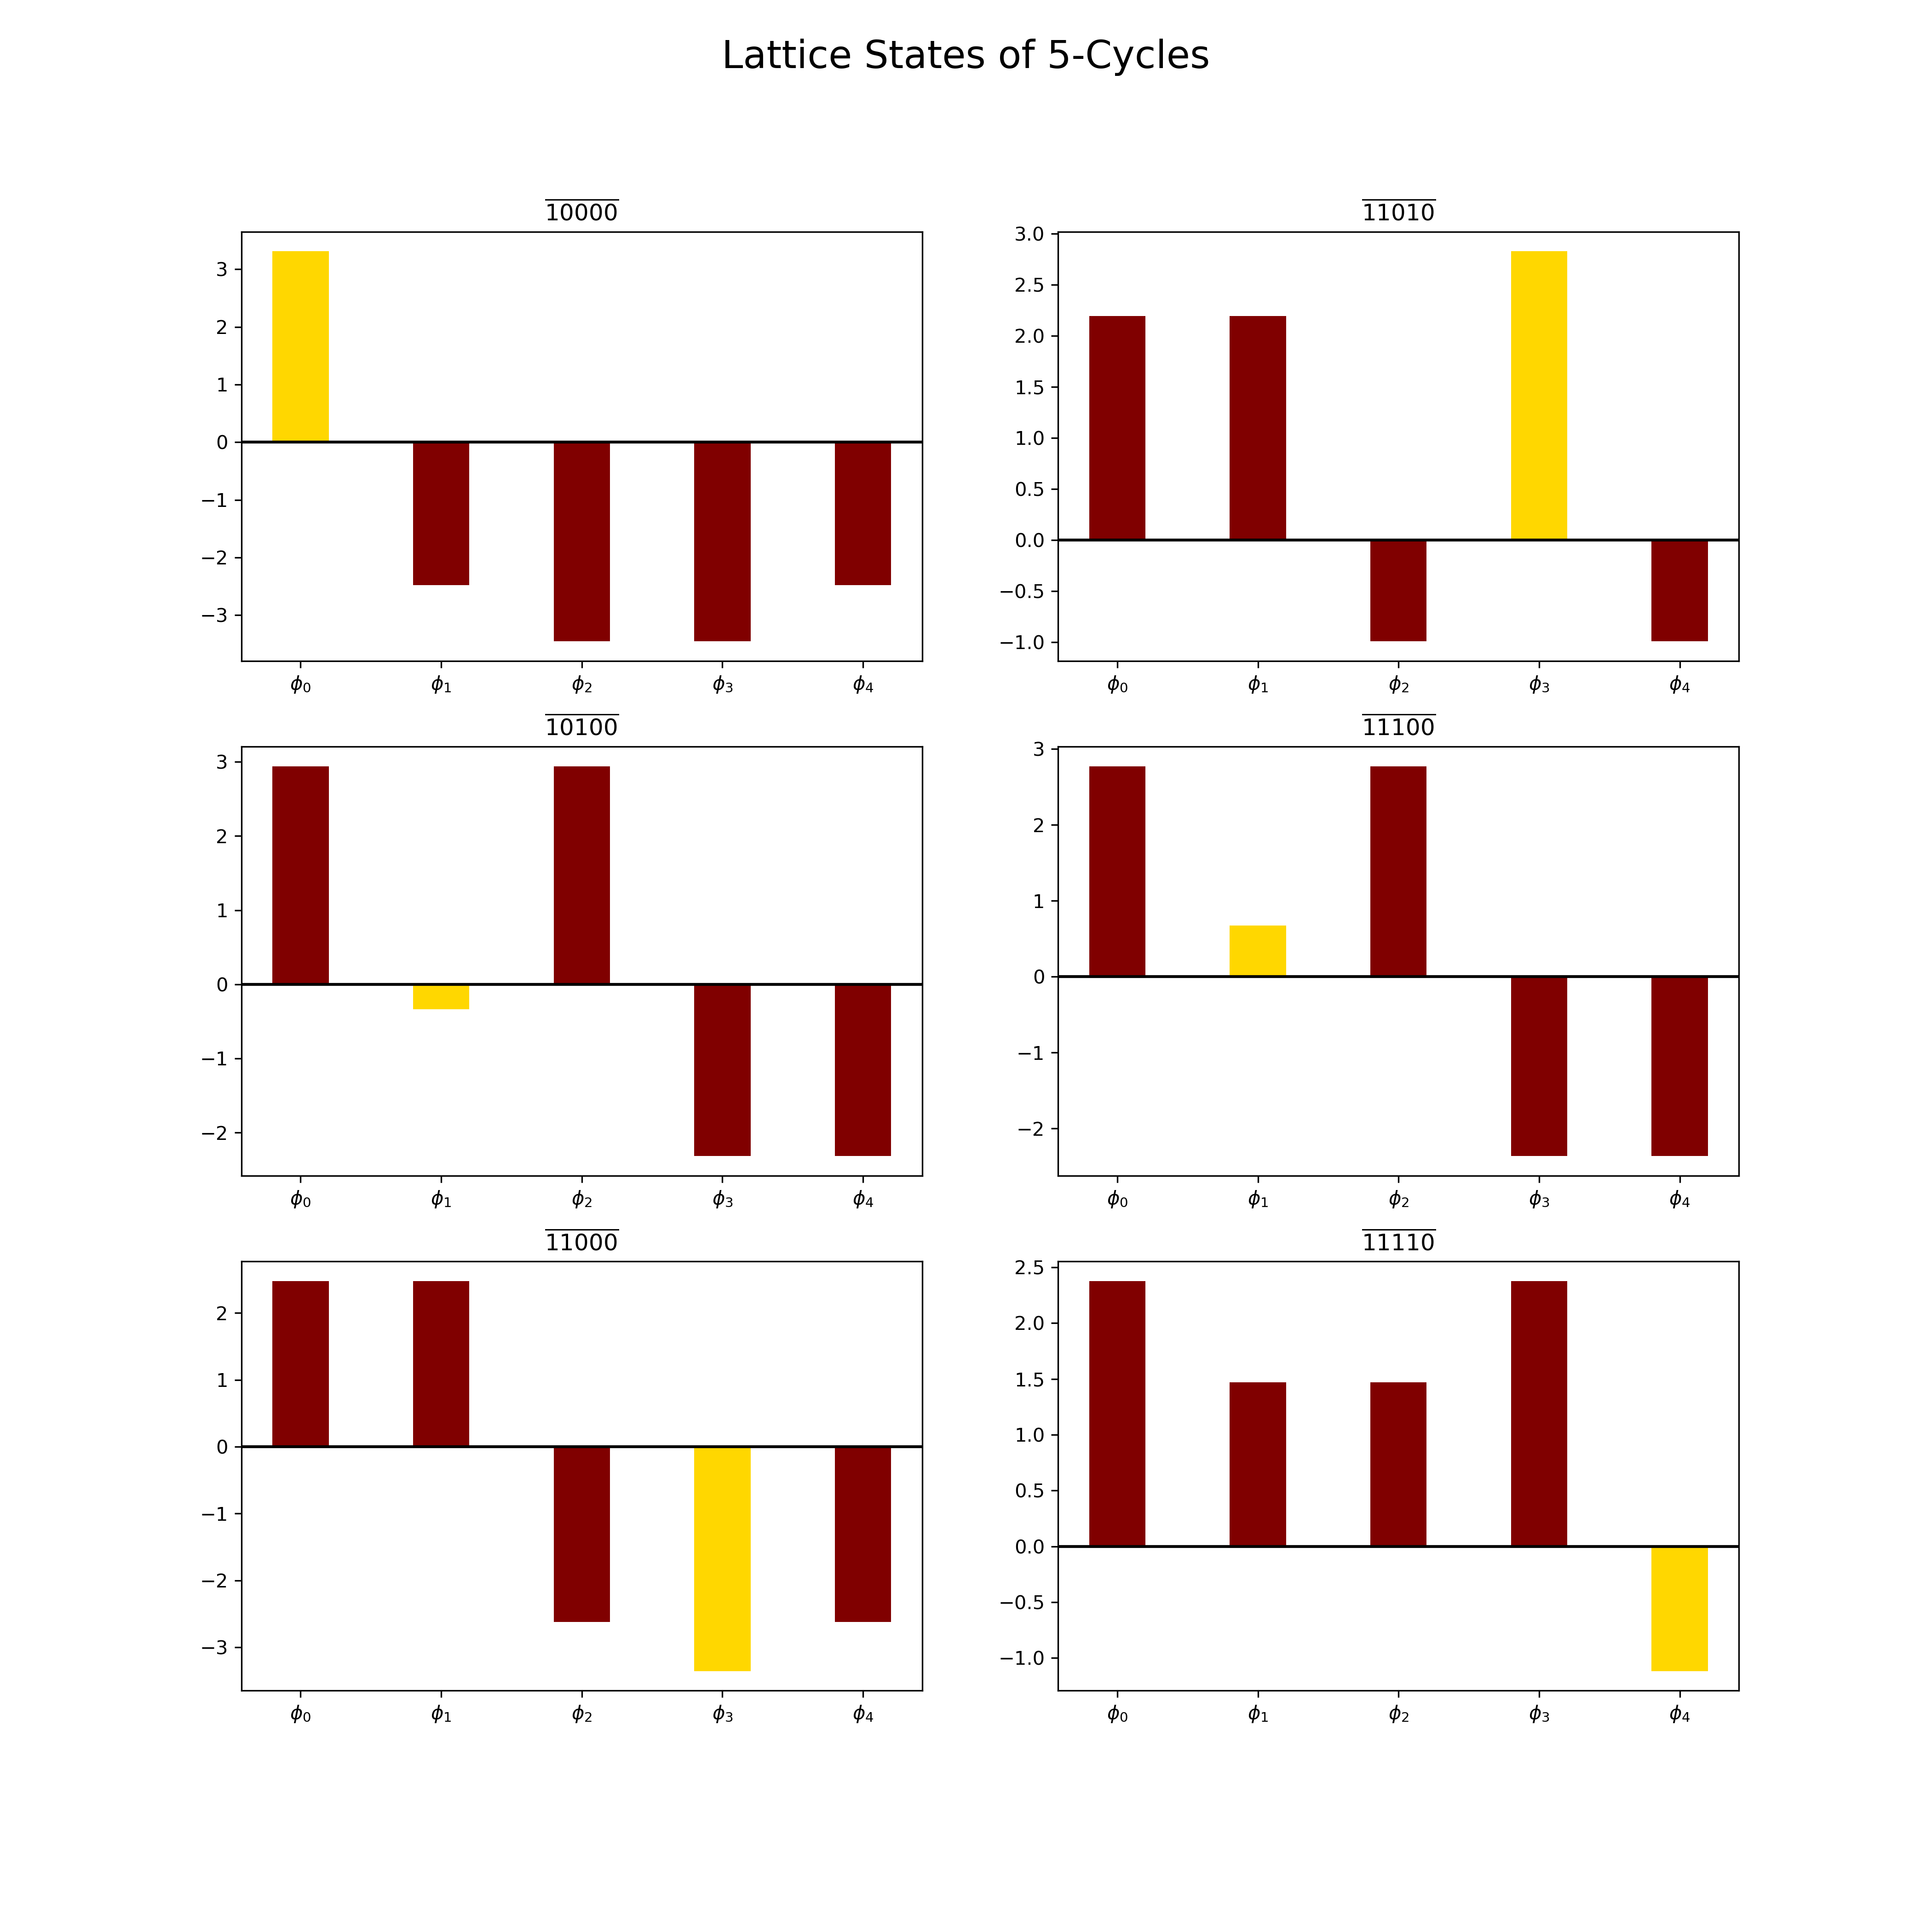
\includegraphics[width=0.45\textwidth]{SVW5latt}
~~~~~~~~
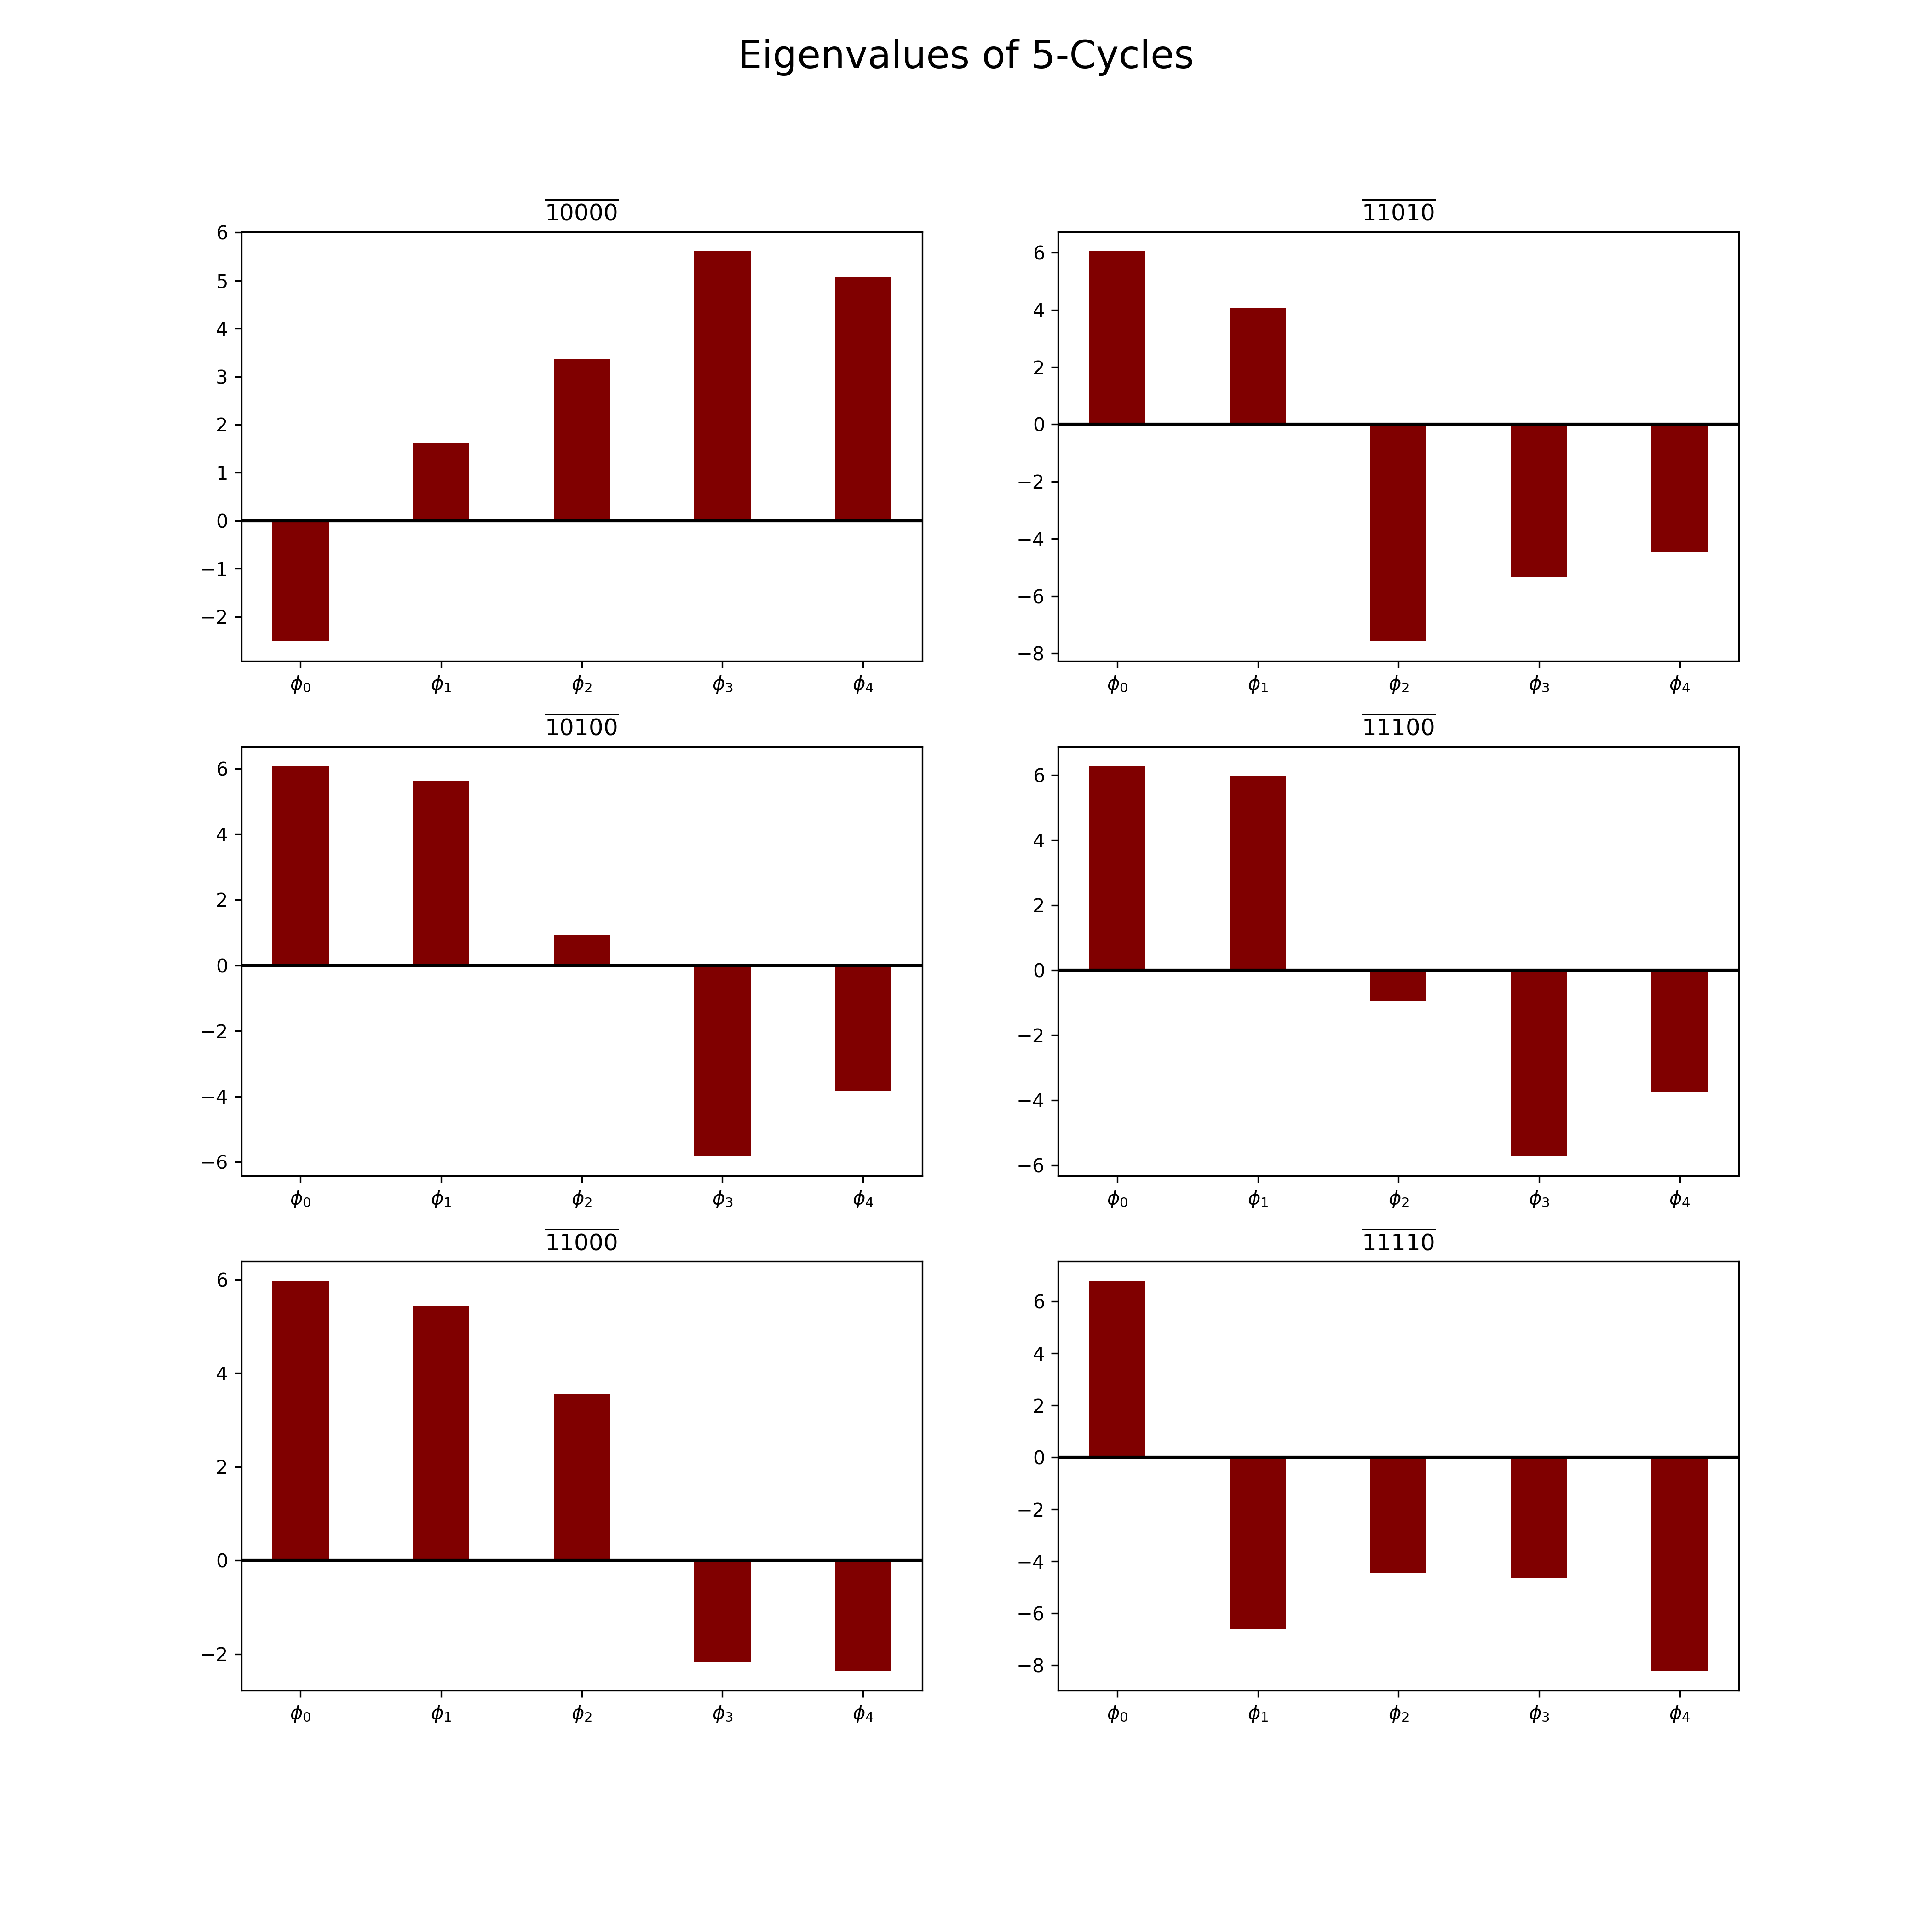
\includegraphics[width=0.45\textwidth]{SVW5eigen}
  \caption{
\Henlatt\ \refeq{Henlatt-2-step}, $a=6$:
(left)
    {\color{red}
The associated {\jacobianOrb}
eigenvalues (?). Currently we have no interpretation. Should't
the corresponding eigenvectors be (anti)symmetric?
    }
}
\label{SVW5CycHamHen}
\end{figure}
%%%%%%%%%%%%%%%%%%%%%%%%%%%%%%%%%%%%%%%%%%%%%%%%%%%%%%%

\item[2021-09-06 Sidney]
I completed the plots for both lattice field values, and the associated
eigenvalues. The formatting is not finished yet, but I will change that
later. Currently, I have the lattice state that remains fixed colored
gold, and the ones that flip colored maroon.

\item[2021-09-07 Predrag].
\begin{enumerate}
  \item
\refFig{SVW5CycHamHen}\,(a) agrees with my own sketch, but only
examination of the actual $\ssp_j$ values can reveal further symmetries and
factorizations.
  \item
\refFig{SVW5CycHamHen}\,(b) currently does
not make much sense to me. 3 of the eigenvalues should belong to
the symmetric subspace \refeq{SVWD5oOrbJac}, \refeq{symmCycD5Proj+},
2 to the antisymmetric subspace  \refeq{symmCycD5Proj-}.
  \item
2021-09-27: \refFig{SVW5CycHamHen}\,(a) is now superseded by
\reffig{fig:PChenlatt5cyc}.
\end{enumerate}


\item[2021-09-06 Sidney]
For a $D_5$ lattice state, the following boundary conditions are respected:
$\ssp_i=\ssp_{i+5}$ and $\ssp_{-i}=\ssp_i$,
if we follow \refeq{symmCycD5eqs}, we find the \henlatt\ {\jacobianOrb} in
the symmetric subspace is
\beq
\jMorb_+=\begin{pmatrix}
2\ssp_0 & 2 & 0\\
1 & 2\ssp_1 & 1\\
0 & 1 & 2\ssp_2+1
\end{pmatrix}
\ee{SVWD5oOrbJac}
As well, from \refeq{symmCycD5eqs}, I can find the 3 equations that
define this sort of orbit for \henlatt
\begin{equation}
\begin{split}
\ssp_0^2+2\ssp_1=a\\
\ssp_0+\ssp_1^2+\ssp_2=a\\
\ssp_1+\ssp^2_2+\ssp_2=a
\end{split}
\end{equation}
Is there a good way of solving this system analytically? Otherwise,
should I just check it by numerically finding solutions?

\item[2021-09-07 Predrag]
No, for us getting into the Endler-Gallas annalytic solutions is getting
too deep into the weeds. Use the same Biham-Wentzel program you have
already written, with the boundary conditions added. The wonderful thing
is that you are looking for the roots of an order $2^3$ polynomial rather
than $2^5$.

To compute the \HillDet\ $\Det\jMorb_+$, Han would recommend doing the
discrete Fourier transform first.

\item[2021-09-07 Predrag]
Currently I prefer the \refeq{LC21:1dHenlatt} form of the \henlatt\ to
\refeq{Henlatt-2-step}, but that is not very important at this stage.

\item[2021-09-07 Sidney]
The full {\jacobianOrb} for the $D_5$ cycles of the \henlatt\ commutes
with reflection about the center lattice state
\refeq{symmCycD5Refl}. Therefore, we can block
diagonalize to find the {\jacobianOrbs} of the symmetric and
antisymmetric subspaces:
\beq
\jMorb_{D_5}=\begin{pmatrix}
2\phi_2-1 & 1 & 0 & 0 & 0\\
1 & 2\phi_1 & 0 & 0 & 0\\
0 & 0 & 2\phi_0 & 2 & 0\\
0 & 0 & 1 & 2\phi_1 & 1\\
0 & 0 & 0 & 1 & 2\phi_2+1\\
\end{pmatrix}
\ee{blockdiagHen5cyc}
Which gives the same matrix for the symmetric subspace as
\refeq{SVWD5oOrbJac}, therefore either boundary conditions or projection
operators are effective for these sort of calculations.

I took a look at my code, and it seems that I wrote it with no
ability to scale $a$, I will fix that, and add in the functionality of
using the traditional field theory formulation and the rescaled "Gallas"
notation that I have been using for awhile.

\item[2021-09-09 Predrag]
You sure about \refeq{blockdiagHen5cyc}? It might be correct, but
how did you derive it?

\item[2021-09-13 Sidney]
I am quite sure of \refeq{blockdiagHen5cyc}. I noticed that the
{\jacobianOrb} for a time reversal invariant orbit commutes with the
$[5\times5]$ reflection matrix
\beq
\Refl =\begin{pmatrix}
0 & 0 & 0 & 0 & 1\\
0 & 0 & 0 & 1 & 0\\
0 & 0 & 1 & 0 & 0\\
0 & 1 & 0 & 0 & 0\\
1 & 0 & 0 & 0 & 0\\
\end{pmatrix}
\ee{55reflect}

So, I found all the eigenvectors associated with \eqref{55reflect} by an
online calculator and and arranged them so that the ones associated with
$-1$ (antisymmetric) and $1$ (symmetric) were grouped together in a
matrix $S$, I then used an online calculator to perform
$$S^{-1}\jMorb S=\jMorb_{BD}$$
And after shuffling around the columns of $S$ (which is allowed for
diagonalization), I got \refeq{blockdiagHen5cyc}.

\item[2021-09-07 Sidney]
This brings me to what
Predrag has asked me to do:

\paragraph{Predrag check list}
\label{PredragChecklistSVW}
\begin{enumerate}
%  \item
%Plot lattice field values for $a>>1$, then try to look at a perturbation
%theory treatment of this.
  \item
I will need to reformulate everything back into the unscaled field values
so that $a$ multiplies the quadratic term.
%  \item
%I will also need to learn some math as I don't know much about the
%perturbative treatments of field theories.
  \item
Find eigenvalues of $D_5$ lattice states in the symmetric subspace to
explain \reffig{SVW5CycHamHen}\,(right).
  \item
Prove that the eigenvalues of the {\jacobianOrb} are metric invariants. I
am stuck here.
  \item
Implement Han's boundary conditions into my code so that I can directly
find orbits with specific symmetries.
\end{enumerate}

%\item[2021-09-09 Predrag]
%Throwing the baby known as \reffig{fig:EG05aCyc5} out with one's LaTeX
%labor learning pains water is not a solution - the baby is there for a reason
%and it is referred to 4 times in the text. I retyped the text by hand -
%does it work for you now?

\item[2021-09-12 Sidney]
%Thank you for fixing \ref{PredragChecklistSVW}, I spent an embarrassing
%amount of time trying to figure out how to both format it nicely, AND
%making is referencable. I think

I will start working on adding boundary
conditions to find different symmetries (a task I have added to the list)
after I clean up my code, and make it easy to switch between Gallas form,
and Field Theory form.

\item[2021-09-13 Sidney]
I have changed my code so that it can be easily switched between
the \Henon\rf{henon} \refeq{PCe_ar_pres}, and Endler and Gallas\rf{EG05}
rescaled \refeq{EG05:ar_pres}, I have added this updated code
\emph{Relaxation Method Henon with Orbit Jacobian.py} to
\emph{siminos/williams/python/relax}.

\item[2021-09-14 Predrag 2 Sidney]
Added \refexer{e-sqrtA}~{\em The matrix square root.}

\item[2021-09-14 Sidney 2 Predrag and Han]
I looked at \refexer{e-sqrtA}~{\em The matrix square root.} I feel
confident in being able to do that. However, I am not sure why I am
looking at the square root here. From what I gathered during today's
meeting, taking the square root of the time-step Jacobian at the boundary
point did not give equality to the hill determinant of the symmetry
reduced {\jacobianOrb}. My impression was that I would instead need to
look for a "square root" of the \henlatt\ is that incorrect?

\item[2021-09-17 Sidney 2 Anyone]
Just for clarification, I should be looking at \eqref{PCperiod7orbJac}
for time symmetric orbits of the \henlatt. I was thinking that since this
is an identity for the forward in time $2\times2$ Jacobian, for orbits
symmetric with respect to time reversal, I would look at the \HillDet\
$\Det \jMorb=\det(\unit-\jMps)$ and check to see that the equality
holds for when I take the half orbit of time-step $\jMps$, compare to the
symmetric part of \eqref{blockdiagHen5cyc}. Is that a good strategy?

\item[2021-09-17 Sidney]
I have completed \refexer{e-sqrtA}, the solution I got on pen
and paper matches the solution that Predrag provided. I will take Andrew
through it tomorrow.

\item[2021-09-17 Sidney]
With respect to adding boundary conditions to my code: I do not know how
to do it as I am not using the Biham-Wentzel method for the \henlatt,
instead (a detail nowhere described in the blog) I invert it  and feed
the code a symbol sequence, see Vattay's \toChaosBook{Item.91} {exercise
7.2}, copied to here as \refexer{exer:HamHenonCyc}.

\item[2021-09-17 Sidney]
I do not know how to
change the boundary conditions.

\item[2021-09-30 Sidney]
The above statement is still true, although, around studying for tests,
and other homework, I been working on testing the formula
\eqref{PCperiod7orbJac} numerically. I have also been review some of the
group theory lectures from over the summer. What I did, was say that the
"factored" time-step Jacobian for a time symmetric period-5 is
\beq
	\tilde{J}=J_2J_1\sqrt{J_0}
\ee{factored5cyc}
Where $\sqrt{J_0}$ can be calculated through the methods worked through in \refexer{e-sqrtA}. I then did the following calculation for every $\sqrt{J_0}$
\beq
	|\Det\jMorb_+|-|\det(I-\tilde{J})|(should)=0
\,,
\ee{reducedHillattempt1}
where $\jMorb_+$ is the $[3\times3]$ block in \eqref{blockdiagHen5cyc}.
This did not work. The closest I got to getting zero was 3.4, which isn't
even an integer. So, I turned to Mathematica, and found that
$\Det\jMorb_+$ has a fundamentally different form from $\det(I-\tilde{J})$
for the \henlatt\ with a time symmetric five cycle, so, I went back to the
drawing board. In the meeting at the beginning of the week, it was
mentioned that the time-step Jacobians had to satisfy the time symmetry
boundary conditions, and my thought was to try to force this by finding
the Jacobian for each equation along a time symmetric period-5 which, with
boundary conditions, yields a 3 equations:
\beq
	2\phi_1+\phi_0^2=a
\ee{symreduct5hen1}
\beq
	\phi_2+\phi_1^2+\phi_0=a
\ee{symreduct5hen2}
\beq
	\phi_2+\phi_2^2+\phi_1=a
\ee{symreduct5hen3}
The time step Jacobian from \eqref{symreduct5hen1} is $J_0=-\phi_0$, and
the time step Jacobian from \eqref{symreduct5hen2} is just the normal one
for the \henlatt. I am not sure how to get a Jacobian out of
\eqref{symreduct5hen3}, perhaps the quadratic equation? If anyone has
suggestions, that would be lovely.

\item[2021-10-05 Sidney]
In this blog entry I describe Vattay's method of determining the
periodic orbits of the Hamiltonian (phase space volume preserving)
\henlatt\ \refeq{pere}, \refexer{exer:HamHenonCyc}~{\em Inverse iteration
method for a {\Henon} repeller}, solution on \refpage{e:pere}.

First, I generate a list of all possible binary itineraries of a given
length. This is a coding exercise, so I will not discuss that here. To
determine the \po s, Vattay inverts the \henlatt\  \refeq{pere} as in
\refeq{GVinver}:
\beq
\ssp_{i}^{(m+1)}=\sign{i}
     \sqrt{\frac{1-\ssp_{i+1}^{(m)}-\ssp_{i-1}^{(m)}}{a}}
\,,
\ee{invertedhen}
where $S_i$ is a sign generated by the symbol sequence. I start the
iteration by setting the initial guess orbit to
$$\ssp_{i}^{(0)}= \sign{i}a^{-1/2}$$
(remember you $a\to\infty$ {\lattstate}s estimates?)
and then evaluating \eqref{invertedhen}.
I then subtract the RHS from the LHS of the
\henlatt\ for each point on the cycle and if it is smaller than a certain
predetermined tolerance, the loop terminates, and the cycle is found. The
meat of the method is contained in these two loops:
{\footnotesize
\begin{verbatim}
for i in range(0,len(symbols)):
	cycle[i]=signs[i]*np.sqrt(abs(1-np.roll(cycle,1)[i]-np.roll(cycle,-1)[i])/a)
for i in range(0,len(symbols)):
	deviation[i]=np.roll(cycle,-1)[i]-(1-a*(cycle[i])**2-np.roll(cycle,1)[i])
\end{verbatim}
}
I could probably set time symmetric boundary conditions in the second
loop, perhaps through an if statement.

I tried stating that \eqref{symreduct5hen3} could be written as
$\phi_{3}=a-\phi_2^2-\phi_1$, which would give just the normal \henlatt\
Jacobian, but it did not match with the determinant of  the $[3\times3]$
block in \eqref{blockdiagHen5cyc}. So my hunch was wrong. Not quite sure
where to go from here in that area.

\item[2021-10-12 Sidney]
I am currently trying to address "Find eigenvalues of $D_5$ lattice
states in the symmetric subspace to explain
\reffig{SVW5CycHamHen}\,(right)." from \ref{PredragChecklistSVW}. I found
a equation for the symmetric part of the {\jacobianOrb} $\jMorb_+$
\eqref{blockdiagHen5cyc}, it is of the form
$a\lambda^3+b\lambda^2+c\lambda+d$ where the coefficients are all
inelegant sums of the lattice field values of a given orbit, it is not
particularly helpful.

\item[2021-10-15 Predrag]
You have to check that the ``inelegant sums'' are invariant under
$\Dn{n}$ symmetries. Han knows and explains how to compute the
eigenvalues and eigenvectors (irreps of \Dn{n}) on the reciprocal
lattice.

I think you will eventually end up with evrything being expressible in
terms of traces of powers of $\Tr \jMorb_+^k$.

I am curious how many {\jacobianOrb} $\jMorb$ eigen-directions are
expanding, what do they look like, stuff like that.

\item[2021-10-12 Sidney]
I think that part of the confusion of the right
hand side of \reffig{SVW5CycHamHen} is that I tried to assign eigenvalues
to individual lattice sites, which is just incorrect, right?

\item[2021-10-15 Predrag]
Eigenvalues are properties of the whole matrix, not a single site.
Only if the matrix is diagonalized are they associates with eigenstates
(`lattice sites' of the reciprocal lattice).

\item[2021-10-12 Sidney]
I am going
to look at \refeq{EG05a(18)} again to see if I can see some pattern. But as
of right now, I think the main conclusion is that the eigenvalues do not
necessarily have the same symmetries as the orbit they belong to.

\item[2021-10-15 Predrag]
Eigen\emph{vectors} have symmetries, not the eigenvalues.

\item[2021-10-25 Sidney]
%After a long time of studying for tests and such (and doing
%troubleshooting)
I have generated some good data for
the eigenstuff, see \reffig{SVW5Cyc11011HamHen}.
%\begin{figure}
%  \centering
%\includegraphics[width=0.90\textwidth]{SVW5latteigvec11011}
%  \caption{
%\Henlatt\ \refeq{Henlatt-2-step}, $a=6$. The eigenvectors of the
%\jacobianOrb\ for the period-5 {\lattstate} $\overline{11011}$, the upper
%left is the cycle itself, and the are the eigenvectors labeled
%by their eigenvalues. The yellow/gold colored bar is the
%lattice site which the state is symmetric or antisymmetric about.
%}
%\label{SVW5Cyc11011HamHen}
%\end{figure}
I need to do further analysis to see which eigenstate(s) is most
important. As well, I think I have some insight into why
\eqref{PCperiod7orbJac} does not work.
The {\jacobianOrb} can be block diagonalized into symmetric and
antisymmetric blocks. As this is the case, Hill's formula can be written
as
$$\Det(\jMorb_-)\Det(\jMorb_+)=\det|I-J|$$
If we assume we can write $J$ as $(J')^2$ (which is what
\eqref{PCperiod7orbJac} assumed), we can then write Hill's formula as
$$\Det(\jMorb_-)\Det(\jMorb_+)=\det|I-J'|\det|I+J'|$$
Which does not imply that $\Det(\jMorb_+)=\det|I-J'|$ which I numerically
showed to be incorrect a few weeks ago. This does not necessarily help
find a correct factorization, but it at least shows us what is wrong.

\item[2021-11-11 Sidney]
I added the plots of the eigenstates for every 5-cycle, as well as the
decomposition for each period lattice state. Unfortunately, there seems to be
no correlation between the important eigenstates and the size of the
eigenvalues.
\item[2021-11-11 Predrag to Sidney].

The figures currently in \emph{siminos/williams/python/Figures/} are not
\emph{*.svg} vector graphics - they are bit images. To see them, download
\HREF{https://inkscape.org/release/all/windows/64-bit/exe/} {Inkscape} and
try to edit them.

\item[2021-11-11 Sidney]
I suppose that almost makes sense because treating the whole
cycle as a fixed point removes iteration from our calculations, perhaps they
will be useful for global stability analysis?
\item[2021-11-11 Predrag to Sidney]
I think so too. Note that as the {\jacobianOrb} is symmetric (at least for the full
Bravais cell - you have to show it also works for the symmetry-reduced case
and $b\neq-1$)
all multipliers $\ExpaEig_j$ are real. Their signs might mean something.


\item[2021-11-11 Predrag to Han].
\begin{enumerate}
  \item
Before Sidney automatizes looking at eigenvectors, what output format do you
prefer?
Sidney's narrow bars as field values, as in \reffig{SVW5CycHamHen},
or Han's fat bars, as in \reffig{fig:PChenlatt5cyc}?
  \item
The problem with \henlatt\ is that due to all period-5 {\lattstate}s being symmetric,
we are getting only 3\dmn\ examples. For \templatt\ you have asymmetric
period-5 {\lattstate}s, there is more information in them.
  \item
Can you take your beloved \templatt\ products of $
\left[s-2\cos\left(\frac{2\pi{j}}{n}\right)\right]$ and do the corresponding
eigenvector plots as
\\
\emph{siminos/williams/python/Figures/} for (some of)
illustrative \templatt\ period-5 {\lattstate}s? Any striking similarities?

\end{enumerate}

\item[2021-11-11 Predrag].

I find the eigenvectors currently in \emph{siminos/williams/python/Figures/}
utterly fascinating.

The $\cl{}$ multipliers $\ExpaEig_j$, $j=1,2,\cdots,\cl{}$ (ChaosBook
reserves the lower case $\lambda_j$ to exponents, but we might change that for
the \spt\ theory) seem all to be of the same
order of magnitude - that will be more apparent when we see their lists for
examples of {\lattstate}s of periods $\cl{}=6,7,8,\cdots$.


\item[2021-12-06 Sidney]
I am still a little unsure how to get the files saved as \emph{*.svg}
vector graphics, the line which saves the pictures is given by

plt.savefig(name+'.svg',dpi=300)

where name is defined earlier in the
code. I am not sure why that does not work. I am also quite close to
automating the cycle finding process with nice looking, and useful
figures, I will do that after finals.

I am still stuck on proving that the eigenvalues of the {\jacobianOrb} are invariant under nonlinear coordinate transforms, the fixed point condition under the field theory just does not seem to allow for it.

I now understand how Han was able to find $2cos(k)-s$ for the eigenvalues, but I am currently having a hard time generalizing that to \henlatt\ I will keep working.

Finally, I have found a (probably useless) tensorial formulation of our theory which allows for the analysis of multiple equation systems (think the Lorenz equations discretized, or \henlatt\ before being compressed into a single equation). It is as follows
\beq
G^{kl}\left[\Phi\right]=\Gamma^{kl}_{ij}\Phi^{ij}+M^{kl}=0^{kl}
\,,
\ee{Multiequationfixed}
Where the index $k$ is for the $k^{th}$ equation, and index $l$ is for the $l^{th}$ lattice point. The index $i$ ranges from 1 to n for a length $n$ orbit, it is the field value on the $l^{th}$ lattice point for the $j^{th}$ variable (think x and y for Henon).
\beq
\Gamma^{kl}_{ij}\equiv\frac{\delta G^{kl}\left[\Phi\right]}{\delta\Phi_{ij}}
\,,
\ee{MultiOrbitJaco}
Several caveats here, I am sure that I could condense this, perhaps combining the $i$ and $l$ index, I am also pretty sure that I messed up the Einstein notation with the co and contravariant indicies. And finally, this is likely completely useless as I am pretty sure that given a system of $k$ first order difference equations, it can be combined into a single higher order equation like what was done with \henlatt\

\item[2021-12-17 Sidney]
I have been trying to get an equation which shows the bounds of the
eigenvalues of the \henlatt\ but the method of just guessing
$e^{\omega^nz}$ doesn't work for the {\jacobianOrb} for \Henon\ because it
does not commute with the shift operator ($\delta_{j+1,k}$), so there is
probably some other $u(z)$ that I need to use, I am not sure though.

\item[2021-12-18 Sidney]
I am trying to establish bounds for the \henlatt. I can do
this numerically, with the minimum value being -0.607625218511 etc. and
the maximum still to be calculated with the code provided for
ChaosBook.org/course1
\HREF{https://phys7224.herokuapp.com/grader/homework7}
{homework 7}. % PHYS 7224.
The stable and unstable
manifolds trace out the region that is bounded ($\Omega$), and the
maxima and minima are determined by their intersections, and I know
that these manifolds can be calculated numerically through forward and
backward iteration, but I feel like I should be able to find these
intersections analytically.
% The best I could come up with, was saying
% that $x_{n+1}=x_{n-1}$ and $y_{n+1}=y_{n-1}$, this does not work, as it
% is simply the condition for length two orbits.
Is there something else
that I could do? Or do I have to resort to numerics?

\item[2021-12-20 Predrag]
I do not believe I have ever seen an analytic expression for a
non-trivial intersection of stable / unstable manifolds. The lower left
corner of \toChaosBook{figure.caption.292} {fig.~15.5} you know
analytically: it is the stability of fixed point \cycle{0}. The upper
right corner of the Smale horseshoe nonwandering set is the heteroclinic
point - lacking something more clever, one might approximate it by the
longest nearby \po, of form \cycle{100\cdots0}. You only need an lower
bound on the magnitude of the multiplier, it's OK to be crude about such
a bound.

An example of \cycle{100\cdots0} sequence of {\po}s is given in
Artuso, Aurell and Cvitanovi\'c
{\em Recycling of strange sets: {II. Applications}}, see their
\HREF{https://cns.gatech.edu/~predrag/papers/AAC-II.pdf} {fig.~2}.
That would correspond to the tangency stretching parameter $a$
value \refeq{LC21:SterlHen}; you are looking at a larger stretching
so there is no funny $\sqrt{\cdots}$ limit in your case, your limit is
cleanly hyperbolic, see \reffig{fig:PChenlatt5cyc}.

\item[2021-09-12 to 2021-09-14, 2021-12-22 Sidney, Predrag]
% It does work for me now, I'm very sorry about the baby...
% I'll be more careful in the future.
It looked like a wild goose chase, so not to distract Sidney further I had
moved the discussion of anti-integrable "perturbation theory" to
\refsect{sect:HamHenonMap}~{\em \Henlatt}.
But it remains of interest: many new references there in
\refsect{sect:HamHenonMap}~{\em {\Henlatt} in anti-integrable limit}.

I have added my guess \refeq{PCphi4} for the infinite coupling $g$
anti-integrable limit of $\phi^4$ theory. That gives a 3-letter
alphabet $\A=\{-1,0,1\}$. One can use it to find by
continuation any {\lattstate}, at $g$ as low as possible.
`Generalized {\HenonMap}s' AKA $\phi^4$ field theory posts are in
\refsect{sect:phi4latt}~{\em Classical {$\phi^4$} lattice field theory}.


\end{description}

\bigskip

\newpage %TEMP
%%%%%%%%%%%%%%%%%%%%%%%%%%%%%%%%%%%%%%%%%%%%%%%%%%%%%%%%%%%%%%%%%%%
% \section{Sidney exercises}
% \label{sect:sidneyExer}
  % $Author: predrag $ $Date: 2021-09-02 23:44:14 -0400 (Thu, 02 Sep 2021) $
% siminos/spatiotemp/Problems/exerHenlatt.tex called by blogSVW.tex

\section{Sidney exercises}
\begin{enumerate} %TEMPORARY
% \Problems{exerHenlatt}{30nov2020}

% Predrag                                               2020-12-27
%  moved GitHub/reducesymm/Problems/exerHenlatt.tex to here
% Predrag                                               2020-11-30

%%%%%%%%%%%%%%%%%%%%%%%%%%%%%%%%%%%%%%%%%%%%%%%%%%%%%%%%%%%%%%%%%%%
\exercise{{\Henon} temporal lattice.}{\label{exer:tempHen}

1\dmn\ temporal {\Henon} lattice (see \toChaosBook{section.3.4} {Example
3.5}) is given by a 3-term recurrence
\beq \nonumber
\ssp_{n+1} + a \ssp_n^2 - b\,\ssp_{n-1} = 1
\,.
\eeq
The parameter $a$ quantifies the ``stretching'' and $b$ quantifies the
``contraction''.

The single H\'enon map is nice because the system is a nonlinear
generalization of \templatt\ 3-term recurrence
CL18 eq.~{catMapNewt}, with no restriction to the unit hypercube XXX, but has
binary dynamics.

There is still a tri-diagonal {\jacobianOrb} $\jMorb$
CL18 eq.~{tempCatFixPoint}, but CL18 eq.~({Hessian}) is now {\lattstate}
dependent. Also, I beleive Han told me that
CL18 sect.~{s:Hill}~{\em {\HillDet}:
            stability of an orbit vs. its time-evolution stability}
block matrices derivation of Hill's formula does not work any more.
Neither does the `fundamental fact', as each {\lattstate}'s {\jacobianOrb}
is different, and presumably does not count periodic states, as there is
no integer lattice within the {\HillDet} volume.

Does the \toChaosBook{section.27.4} {flow conservation} sum rule
\toChaosBook{equation.27.4.15}{ed.~(27.15)}
(or CL18.tex eq.~{Det(jMorb)eights}) still work?

The assignment: Implement the variational searches for
periodic states in Matt's \HREF{https://github.com/farom57/Orbit-hunter}
{OrbitHunter}, find all {\lattstate}s up to $n=6$.

(a) $a=1.4\,\;b=0.3$, compare with
\toChaosBook{table.caption.559} {Table~34.2}.

(b) For $b=-1$ the system is time-reversible or `Hamiltonian',
see
\toChaosBook{exmple.8.5}{Example 8.5}.
For definitiveness, in numerical calculations in examples to follow we
fix (arbitrarily) the stretching parameter value to $a=6$, a value large
enough to guarantee that all roots of the periodic point condition
$0=f^n(x)-x$  are real.

Note also
\toChaosBook{section.J.3}
{sect~A10.3} {\em H\'enon map symmetries}
and
\toChaosBook{Item.91}
{Exer.~7.2} {\em Inverse iteration method}.

The deviation of an approximate trajectory from the 3-term recurrence is
\beq \nonumber
v_n = \ssp_{n+1} - (1 - a \ssp_n^2 + b\,\ssp_{n-1})
\eeq
In classical mechanics force is the gradient of a potential, which
Biham-Wenzel\rf{afind} construct as a cubic potential
\beq
V_n = \ssp_{n+1}\ssp_n - b\,\ssp_n\ssp_{n-1} + (a \ssp_n^3 - \ssp_n)
\,.
\ee{BWcubic}
With the cubic potential at lattice site $n$ we can start to look for
orbits variationally. Note that the potential is time-reversal invariant
for $b=1$.


Compare with XXX
    } % end \exercise{exer:catMapGreenInf}
%%%%%%%%%%%%%%%%%%%%%%%%%%%%%%%%%%%%%%%%%%%%%%%%%%%%%%%%%%%%%%%%%%%%%%%%

%%%%%%%%%%%%%%%%%%%%%%%%%%%%%%%%%%%%%%%%%%%%%%%%%%%%%%%%%%%%%%%%%%%
%\exercise{XXX.}{\label{exer:XXX}
%XXX
%    } % end \exercise{exer:XXX}
%%%%%%%%%%%%%%%%%%%%%%%%%%%%%%%%%%%%%%%%%%%%%%%%%%%%%%%%%%%%%%%%%%%%%%%%

%%%%%%%%%%%%%%%%%%%%%%%%%%%%%%%%%%%%%%%%%%%%%%%%%%%%%%%%%%%%%%%%%%%
%\exercise{XXX.}{\label{exer:XXX}
%XXX
%    } % end \exercise{exer:XXX}
%%%%%%%%%%%%%%%%%%%%%%%%%%%%%%%%%%%%%%%%%%%%%%%%%%%%%%%%%%%%%%%%%%%%%%%%

% \end{enumerate} %TEMPORARY, moved to exerGroupThe.tex
%    \ProblemsEnd

  % siminos/spatiotemp/Problems/exerGroupThe.tex called by blogSVW.tex
% $Author: predrag $ $Date: 2021-09-14 18:16:58 -0400 (Tue, 14 Sep 2021) $


% \Problems{exerGroupThe}{6mar2021}

%%%%%%%%%%%%%%%%%%%%%%%%%%%%%%%%%%%%%%%%%%%%%%%%%%%%%%%%%%%%%%%%%%%
% Sidney                        2021-03-07
\exercise{Engel Point Groups 1.}{\label{exer:Engel11PG1}
(Engel's\rf{Engel11}
\HREF{http://www-personal.umich.edu/~engelmm/lectures/ShortCourseSymmetry1.pdf}
{Point Groups} Exercise 1):
The molecule on the left has $C_{1s}$ which signifies
that it has reflection symmetry over one axis. The molecule on the right
has $C_3$ symmetry, signifying that it is symmetric by rotations of
$\frac{2\pi}{3}$ or one third of a full circle.

\hfill M.~Engel
    } % end \exercise{exer:Engel11PG1}
%%%%%%%%%%%%%%%%%%%%%%%%%%%%%%%%%%%%%%%%%%%%%%%%%%%%%%%%%%%%%%%%%%%

%%%%%%%%%%%%%%%%%%%%%%%%%%%%%%%%%%%%%%%%%%%%%%%%%%%%%%%%%%%%%%%%%%%
% Sidney                        2021-03-07
\exercise{Engel Point Groups 3.}{\label{exer:Engel11PG3}
(Engel's\rf{Engel11}
\HREF{http://www-personal.umich.edu/~engelmm/lectures/ShortCourseSymmetry1.pdf}
{Point Groups} Exercise 3):
Three point groups for $C_2H_6$: a. $C_{3v}$ because rotating it by 1/3
of a circle leaves it invariant, and one can cut the molecules into three
identical pieces. b. $C_s$ because the top and bottom have the same
orientation, it is like looking in a mirror, so can apply reflection
symmetry. c. Unsure, perhaps inversion symmetry $C_i$.

\hfill M.~Engel
    } % end \exercise{exer:Engel11PG3}
%%%%%%%%%%%%%%%%%%%%%%%%%%%%%%%%%%%%%%%%%%%%%%%%%%%%%%%%%%%%%%%%%%%

  % siminos/spatiotemp/Problems/exerSqrtA.tex called by blogSVW.tex
% $Author: predrag $ $Date: 2021-09-14 18:16:58 -0400 (Tue, 14 Sep 2021) $

%%%%%%%%%%%%%%%%%%%%%%%%%%%%%%%%%%%%%%%%%%%%%%%%%%%%%%%%%%%%%%%%%%%%%
\exercise{The matrix square root.}{  \label{e-sqrtA}
% copied from 2021-08-08 PHYS-7143-21/notes/problems/exerWeek1.tex
% From Golub and Van Loan\rf{GoVanLo96} sect 9.4.2
%                                            \inCB
Consider matrix
\[
A=
\MatrixII{4}{10}
         {0}{9}
\,.
\]
Generalize the square root function $f(x)=x^{1/2}$ to
a square root  $f(A)=A^{1/2}$ of a matrix $A$.
\\
a) Which one(s) of these is/are the square root of $A$
\[
\MatrixII{2}{2}
         {0}{3}
\;,
\MatrixII{-2}{10}
         {0}{3}
\;,
\MatrixII{-2}{-2}
         {0}{-3}
\;,
\MatrixII{2}{-10}
         {0}{-3}
\;\,?
\]
b) Assume that the eigenvalues of a [$d\times{d}$] matrix are all
   distinct. How many square root matrices does such matrix have?
   \\
c) Given a [2$\times$2] matrix $A$ with a distinct pair of eigenvalues
   $\{\lambda_1,\lambda_2\}$, write down a formula that generates
   all square root matrices $A^{1/2}$. Hint: one can do this
   using the 2 projection operators associated with the matrix $A$.
   \hfill 2 points
    } % end \exercise{The matrix square root.}{
%%%%%%%%%%%%%%%%%%%%%%%%%%%%%%%%%%%%%%%%%%%%%%%%%%%%%%%%%%%%%%%%%%%%%

\end{enumerate} %TEMPORARY,starts in exerHenlatt.tex
%    \ProblemsEnd

  % $Author: predrag $ $Date: 2021-12-20 09:38:42 -0500 (Mon, 20 Dec 2021) $
% siminos/spatiotemp/Solutions/soluHenlatt.tex called by blogSVW.tex

% \section{Sidney solutions}  % TEMPORARY
% \Solution{blogSVW}{soluHenlatt}{23jan2018}{Sidney's blog}

% Predrag                                               2020-12-27
%  moved GitHub/reducesymm/Solutions/soluHenlatt.tex to here
% Predrag                                               2020-11-30

%%%%%%%%%%%%%%%%%%%%%%%%%%%%%%%%%%%%%%%%%%%%%%%%%%%%%%%%%%%%%%%%%%%
\solution{exer:tempHen}{H\'enon temporal lattice.}{

(a) Here's my initial attempt, I'm trying to see if the flow conservation
law CL18 eq.~{Det(jMorb)eights} still works for the {\Henon} map:
$$\phi_{n+1}+a\phi^2_n-b\phi_{n-1}=1$$
The first step seems to be to construct the {\jacobianOrb} $\mathcal{J}$:
\begin{equation}\label{1}
F[\mathbf{\Phi}]=\mathcal{J}\mathbf{\Phi}-I
\end{equation}
Where $I$ is the identity matrix, and $F$ is the function where we want to find the zeros for (the orbits). We can rewrite this as:
\begin{equation}\label{2}
\left(\sigma+aI\mathbf{\Phi}-b\sigma^{-1}\right)\mathbf{\Phi}=I
\end{equation}
Therefore, $\mathcal{J}$ is
\begin{equation}\label{3}
\mathcal{J}=\sigma+aI\mathbf{\Phi}-b\sigma^{-1}=
  \left[ {\begin{array}{ccccc}
   a\phi_1 & 1 & 0 & \cdots & -b \\
   -b & a\phi_2 & 1 & \cdots & 0 \\
   0 & \ddots & \ddots & \ddots & \vdots \\
   \vdots & \cdots & -b & a\phi_{n-1} & 1 \\
   1 & 0 & \cdots & -b & a\phi_n\\
  \end{array} } \right]
\end{equation}

Before I take a crack at seeing if this flow conservation still holds, I do have some questions:
\begin{itemize}
\item[Q1 Sidney]
It appears that the derivation from chapter 23 (eqn 23.17, I don't know
how to cite that specifically) the denominator of the sum rule is a
product of the eigenvalues $\Lambda_{pi}$, which (if I remember
correctly) are just the eigenvalues of the {\jacobianOrb} of the flow or
map, which from basic linear algebra I know to be just the determinant of
the {\jacobianOrb}. It cannot be that straightforward, where is the flaw
in my logic?

\item[Q2 Sidney]
How do I go from the periodic orbit formulation of the sum rule from Ch 23 to the lattice formulation? My initial thought is that since {\lattstate}s are akin to a periodic orbit (right?) that the sum can just be immediately changed from a sum over all periodic orbits, to a sum over all {\lattstate}s. Is this reasoning correct?

\item[Comment Sidney]
I now realize that the flow sum rule involving the {\jacobianOrb} (NOT the Hill matrix) is a fundamental property that applies to all systems (at least all closed systems), what I now know is that I need to work out if I can convert between the determinant of the {\jacobianOrb} and the determinant of the Hill matrix.

\item[Plan Sidney]
I am going to try to see what I can do with the block matrix proof, and I will get back to everyone on Friday

\item[Update Sidney]
I tried working out the proof with the block matrices for just the
regular Bernoulli map, I understand everything except the sentence "For a
period-$\cl{}$ {\lattstate} $\mathbf{\Phi}_M$, the {\jacobianOrb}
(15) is now a $[ndXnd]$ matrix function of the $[dXd]$ block matrix J."
It sort of seemed like it was much like "poof! And then a miracle
happens!" I will keep exploring.

I shall now correct my mistake with the derivation of the {\jacobianOrb}/Hill matrix $\mathcal{J}$ I shall use the differential definition:
$$\mathcal{J}_{ij}=\frac{\delta F[\Phi]_j}{\delta\phi_i}$$
Which gives us that $\mathcal{J}=\sigma+2aI\Phi_n-b\sigma^{-1}$. Now I will use the differential definition of the local Jacobian, where f is a functions such that $f(\phi_n)=\phi_{n+1}$
$$J_{ij}=\frac{\partial f(\phi_n)_i}{\partial \phi_{nj}}$$
Which gives us that $J(\phi_n)=-2a\phi_n$. So we can rewrite $\mathcal{J}=\sigma-J(phi_n)I-b\sigma^{-1}$, with the understanding that J changes along the diagonal. I am not quite sure how to bring this to the sum rule, but I will soon (hopefully), how do I math things like $\phi\text{ and }\Phi$ bold?

\item[Update Sidney]
I need to do a proper mathematical look at the flow conservation, but the
H\'enon map is not flow conserving (some trajectories are inadmissible)
so the sum rule does not equal $1$, I will try later to look at what it
does equal analytically, but until then I will tackle the computation. I
have made great progress with that, with help from Matt I was able to
create a working code that gave me the correct {\orbit}s up to length
10 (I could not check past that). The code is in my blog. Once Matt has
completed the current round of OrbitHunter updates I shall try to use
that to reproduce my results.

\item[Solution Sidney]
(a) The flow conservation sum rule does not sum to $1$ so it does not
work as before, I still need to try to relate the global Hill matrix to
the local Jacobian matrix, I think I may be close to reworking the block
matrix proof. Anyway, here are the periodic points I found (please note
that the code cannot be used to find fixed points (n=1) so I just did it
analytically, I will try to add that to the code later):
$$n=1\quad -1.13135447$$
$$n=1\quad 0.63135447$$
$$n=2\quad [0.97580005, -0.47580005]$$
$$n=4\quad [1.12506994,-0.70676678,0.63819399,0.21776177]$$
$$n=6\quad [1.03805954, -0.41515894, 1.07011813, -0.72776163, 0.57954366, 0.31145232]$$
$$n=6\quad [1.1579582, -0.8042199, 0.44190995, 0.48533586, 0.80280173, 0.2433139]$$
When I tried to find $n=3$ and $n=5$ the code returned nothing, this
matches with what is tabulated in table 34.2. I will try using some of
the analytical pruning techniques to prove that $n=3$ and $n=5$ are not
allowed.

\end{itemize}
\hfill (Sidney Williams 2021-01-20)
    } % end \solution{exer:catMapGreenInf}
%%%%%%%%%%%%%%%%%%%%%%%%%%%%%%%%%%%%%%%%%%%%%%%%%%%%%%%%%%%%%%%%%%%%%%%%

  % siminos/spatiotemp/Solutions/soluGroupThe.tex called by blogSVW.tex
% $Author: predrag $ $Date: 2021-04-26 02:01:31 -0400 (Mon, 26 Apr 2021) $

% \section{Sidney solutions}  % TEMPORARY
% \Solution{blogSVW}{soluGroupThe}{23jan2018}{Sidney's blog}

% Sidney                        2021-03-07
%%%%%%%%%%%%%%%%%%%%%%%%%%%%%%%%%%%%%%%%%%%%%%%%%%%%%%%%%%%%%%%%%%%
\solution{exer:Engel11PG1}{Engel Point Groups 1.}{
The molecule on the left has $C_i$ symmetry which is inversion symmetry
NOT reflection symmetry because the top and bottom arrangements are not
like they would be if placed in front of a mirror. The molecule on the
right has $C_{3v}$ symmetry, which is pyramidal symmetry which
corresponds to the fact that one could take three slices of the molecule
and they would each be identical, not just the configuration would be
preserved by a rotation.

\hfill (Sidney Williams 2021-03-07)
    } % end \solution{exer:Engel11PG1}
%%%%%%%%%%%%%%%%%%%%%%%%%%%%%%%%%%%%%%%%%%%%%%%%%%%%%%%%%%%%%%%%%%%%%%%%

% Sidney                        2021-03-07
%%%%%%%%%%%%%%%%%%%%%%%%%%%%%%%%%%%%%%%%%%%%%%%%%%%%%%%%%%%%%%%%%%%
\solution{exer:Engel11PG3}{Engel Point Groups 3.}{
Apparently, it depends based on whether we are dealing with staggered
Ethane or not. If it is staggered, then it has inversion symmetry, if it
is not, it has reflection symmetry, it should have $C_{3}$ symmetry
instead of $C_{3v}$ which confuses me a great deal. If I remember
correctly it should correspond to a reflection vertical plane, which it
should have, so I do not understand. The third one is $C_2$ which I do
not understand how it is different from the inversion symmetry. Although,
looking at simulations from
\HREF{https://www.chemtube3d.com/sym-ethanestaggered/}{here}, it looks
like the $C_2$ group can be used to rotate about axes that are different
in orientation from just right through the middle.
\hfill (Sidney Williams) 2021-03-07
    } % end \solution{exer:Engel11PG3}
%%%%%%%%%%%%%%%%%%%%%%%%%%%%%%%%%%%%%%%%%%%%%%%%%%%%%%%%%%%%%%%%%%%%%%%%

  % siminos/spatiotemp/Solutions/soluSqrtA.tex  called by blogSVW.tex
% $Author: predrag $ $Date: 2021-09-14 18:16:58 -0400 (Tue, 14 Sep 2021) $

%%%%%%%%%%%%%%%%%%%%%%%%%%%%%%%%%%%%%%%%%%%%%%%%%%%%%%%%%%%%%%%%%
% From Golub and Van Loan\rf{GoVanLo96} sect 9.4.2
% copied from PHYS-7143-21/notes/solutions/soluWeek1.tex
% Predrag                                   2020-08-19
\solution{e-sqrtA}{The matrix square root.}{.
                                            \inCB

\noindent
a) It is easy to check that
\[
A = \left[\begin{array}{cc}
 4 & 10 \\
 0 & 9
\end{array}\right]
  = \left(A_{ij}^{1/2}\right)^2
\]
for the matrices
\bea
A^{1/2}_{++}&=&\left[\begin{array}{cc}
 2 & 2 \\
 0 & 3 \\
\end{array}\right]
    \,,\quad\quad\;\;
A^{1/2}_{+-}=\left[\begin{array}{cc}
 -2 & 10 \\
 0 & 3 \\
\end{array} \right]
\continue
A^{1/2}_{--}&=&\left[
\begin{array}{cc}
 -2 & -2 \\
 0 & -3 \\
\end{array}\right]
    \,,\quad
A^{1/2}_{-+}=\left[
\begin{array}{cc}
 2 & -10 \\
 0 & -3 \\
\end{array}\right]
\label{ProjOp2d-pm}
\eea
Being upper-triangular, the eigenvalues of the four matrices
can be read off their diagonals:
there are four square root $\pm$ eigenvalue combinations
$\{$3,2$\}$, $\{$-3,2$\}$, $\{$3,-2$\}$, and $\{$-3,-2$\}$.

Associated with each set $\lambda_i\in\{\lambda_1,\lambda_2\}$
is the {\em projection operator}
%\refeq{2dEigVec} %RESTORE
\bea
\PP^{(1)}_{ij} &=& \frac{1}{\lambda_1-\lambda_2} (A_{ij}^{1/2} - \lambda_2\matId)
\,=\, \MatrixII{0}{2}
               {0}{1}
\label{ProjOp2d(1)} \\
\PP^{(2)}_{ij} &=& \frac{1}{\lambda_2-\lambda_1}(A_{ij}^{1/2} -\lambda_1\matId)
\,=\, \MatrixII{1}{-2}
               {0}{ 0}
\,.
\label{ProjOp2d(2)}
\eea
Note that all {`}square root{'} matrices have the
same projection operators / eigenvectors as the matrix $A$ itself, so
one can drop the $ij$ subscripts on $\PP^{(1)},\PP^{(2)}$.

\noindent
b) If the eigenvalues of  a [$d\times{d}$] matrix are all distinct,
the matrix is diagonalizable, so
the number of square root $\pm$ combinations is $2^d$.
However, for general matrices things can get crazy - there can be
\HREF{https://en.wikipedia.org/wiki/Square_root_of_a_matrix}
{no, or some, or $\infty$} of `square root' matrices.

\noindent
c)  We
know $\{\lambda_1,\lambda_2\}$ and $\PP^{(\alpha)}$ for $A$, and the four
`square root' eigenvalues are clearly
$\{\pm\lambda_1^{1/2},\pm\lambda_2^{1/2}\}$. That suggest finding the
`square root' matrices \refeq{ProjOp2d-pm} by reverse-engineering
\refeq{ProjOp2d(1)}, \refeq{ProjOp2d(2)}:
\[
A_{ij}^{1/2} =(\lambda_1-\lambda_2)\PP^{(1)}  + \lambda_2\matId
\,,
\]
which is, of course, how the problem was cooked up.
For example,
\[
A_{+-}^{1/2}
 = (+3-(-2))\MatrixII{0}{2}
                     {0}{1}
  + (-2)\MatrixII{1}{0}
                 {0}{1}
\,.
\]
    } %end \solution{e-sqrtA}
%%%%%%%%%%%%%%%%%%%%%%%%%%%%%%%%%%%%%%%%%%%%%%%%%%%%%%%%%%%%%%%%%


\renewcommand{\ssp}{\ensuremath{x}}             % lattice site field
\renewcommand{\Ssym}[1]{{\ensuremath{s_{#1}}}}    % Boris
\renewcommand{\Refl}{\ensuremath{\sigma}}             % in DasBuch
\renewcommand{\shift}{\ensuremath{d}}                 % in DasBuch

%%%%%%%%%%%%%%%%%%%%%%%%%%%%%%%%%%%%%%%%%%%%%%%%
\printbibliography[heading=subbibintoc,title={References}]

\ChapterEnd % formatted for ChaosBook.org
